%% Manuscript for Expert Systems with Applications (Elsevier CAS template, single column).
%% Build:  latexmk -pdf main.tex   (or: pdflatex main && bibtex main && pdflatex main && pdflatex main)
%% Layout check with simulated numbers (never for submission):
%%   pdflatex "\def\gendir{generated_sim}%% Manuscript for Expert Systems with Applications (Elsevier CAS template, single column).
%% Build:  latexmk -pdf main.tex   (or: pdflatex main && bibtex main && pdflatex main && pdflatex main)
%% Layout check with simulated numbers (never for submission):
%%   pdflatex "\def\gendir{generated_sim}%% Manuscript for Expert Systems with Applications (Elsevier CAS template, single column).
%% Build:  latexmk -pdf main.tex   (or: pdflatex main && bibtex main && pdflatex main && pdflatex main)
%% Layout check with simulated numbers (never for submission):
%%   pdflatex "\def\gendir{generated_sim}%% Manuscript for Expert Systems with Applications (Elsevier CAS template, single column).
%% Build:  latexmk -pdf main.tex   (or: pdflatex main && bibtex main && pdflatex main && pdflatex main)
%% Layout check with simulated numbers (never for submission):
%%   pdflatex "\def\gendir{generated_sim}\input{main}"
\documentclass[a4paper,fleqn]{cas-sc}

\usepackage[authoryear,longnamesfirst]{natbib}
\usepackage{amsmath,amssymb,amsthm}
\usepackage{booktabs,multirow,makecell}
\usepackage{graphicx}
\usepackage{xcolor}
\usepackage[ruled,linesnumbered,vlined]{algorithm2e}
\usepackage{tikz}
\usetikzlibrary{arrows.meta,positioning,shapes.geometric,shapes.symbols,fit,backgrounds,calc}
\usepackage{enumitem}
\usepackage{siunitx}

\newtheorem{proposition}{Proposition}
\newtheorem{lemma}{Lemma}
\theoremstyle{definition}
\newtheorem{definition}{Definition}

%% ---------------------------------------------------------------------------------------
%% Numbers produced by the experiment pipeline (scripts/make_paper_assets.py, data_stats.py).
%% Missing values are printed as red placeholders, so nothing is ever typed in by hand.
\providecommand{\gendir}{generated}
\newcommand{\tbd}[1]{\textcolor{red}{[\detokenize{#1}]}}
\newcommand{\res}[1]{\ifcsname res@#1\endcsname\csname res@#1\endcsname\else\tbd{#1}\fi}
\InputIfFileExists{generated/data_numbers.tex}{}{}
\InputIfFileExists{\gendir/numbers.tex}{}{}
\newcommand{\gentable}[1]{\IfFileExists{\gendir/#1.tex}{\input{\gendir/#1}}{\tbd{#1: pending Jev run}}}
\newcommand{\genfigure}[2][\textwidth]{\IfFileExists{\gendir/#2.pdf}{\includegraphics[width=#1]{\gendir/#2}}{\fbox{\parbox{0.9\textwidth}{\centering\tbd{#2: pending Jev run}}}}}
\ifdefined\SimulatedResults
  \AddToHook{shipout/background}{\put(0.5\paperwidth,-0.5\paperheight){\makebox(0,0){\rotatebox{45}{\fontsize{40}{40}\selectfont\color{red!25}SIMULATED -- LAYOUT ONLY}}}}
\fi

\newcommand{\feel}[1]{\texttt{#1}}
\newcommand{\jev}{Jev}

\begin{document}
\let\WriteBookmarks\relax
\def\floatpagepagefraction{1}
\def\textpagefraction{.001}

\shorttitle{Distilling typed probabilistic decisions into DMN}
\shortauthors{D. Etinger}

\title[mode=title]{From typed probabilistic answers to auditable decision tables: distilling a System One model into DMN with risk-controlled automation}

\author[1]{Darko Etinger}[orcid=0000-0003-4444-7202]
\cormark[1]
\ead{darko.etinger@unipu.hr}
\credit{Conceptualization, Methodology, Software, Investigation, Writing -- original draft, Writing -- review \& editing}

%% TODO(authors): confirm Nikola Tanković's CRediT roles (placeholder below).
\author[1]{Nikola Tankovi\'c}[orcid=0000-0003-3936-1244]
\ead{nikola.tankovic@unipu.hr}
\credit{Writing -- review \& editing}

\affiliation[1]{organization={Juraj Dobrila University of Pula, Faculty of Informatics},
  addressline={Zagreba\v{c}ka 30},
  postcode={52100},
  city={Pula},
  country={Croatia}}

\cortext[1]{Corresponding author}

\begin{abstract}
Operational decisions in business processes increasingly start from unstructured input, such as complaints, e-mails or claims, that rule-based decision models cannot read. Language models can read such input, but their decision logic cannot be audited, and it is unclear when their output may be acted on without a human. We study a new class of models, System One models, which answer a fixed set of typed questions (choices, yes/no statements, ordinal scores) with a probability distribution for each answer, and show how to turn such a model into an auditable and executable decision service based on the Decision Model and Notation (DMN) standard. The model serves twice: as a teacher, whose holistic decisions on unlabelled cases are distilled into a DMN decision table over its own typed answers, and as a source of uncertainty, whose probabilities feed a confidence gate. The table is verified for overlaps and gaps and checked against an independent FEEL engine. The gate is learned from a small labelled set, and its threshold is chosen with Learn-then-Test, so that the error rate of automatically decided cases stays below a chosen level with high probability. We evaluate the approach with Jev, a commercial System One model, on \res{data.sample} consumer complaints from the Consumer Financial Protection Bureau in two tasks: deciding monetary relief and routing complaints to handling queues. We report the fidelity and size of the distilled tables, the calibration of the model's probabilities, the share of cases that can be automated at error levels between 1\% and 10\%, and the accuracy, latency and cost of the approach against the model alone and against supervised baselines.
\end{abstract}

\begin{highlights}
\item A typed probabilistic model is distilled into a verified DMN decision table.
\item The model's probabilities drive a learned confidence gate expressed in DMN.
\item Learn-then-Test thresholds bound the error rate of automated cases.
\item Exported decision models are XSD-valid and agree with an independent FEEL engine.
\item Evaluated on 17,674 CFPB complaints in two complaint-handling decisions.
\end{highlights}

\begin{keywords}
Decision Model and Notation \sep
Business process management \sep
Knowledge distillation \sep
Selective classification \sep
Risk control \sep
Human-in-the-loop automation
\end{keywords}

\maketitle

%% =======================================================================================
\section{Introduction}\label{sec:intro}

Operational decisions, such as approving a refund, routing a request or escalating a claim, are where business processes create or destroy value at scale \citep{dumas2018}. The Decision Model and Notation (DMN) standard \citep{omg_dmn13} separates such decisions from process control flow and expresses them as decision tables whose rules business analysts can read, test and change, and which process engines execute directly \citep{hasic2018,figl2018}. Decision tables have a well-defined semantics, so overlapping and missing rules can be detected automatically \citep{calvanese2016,calvanese2018}. These properties make DMN attractive wherever decisions must be explained to customers, auditors or regulators. In the European Union, for example, high-risk AI systems must be transparent to their deployers and allow effective human oversight \citep{euaiact2024}.

Decision tables, however, can only read structured data. A growing share of process instances starts from unstructured input: a complaint narrative, an e-mail, a call transcript, a claim description. Machine learning, and recently large language models (LLMs), can read such input \citep{vidgof2023}, but they put the decision logic in a black box, and their confidence statements are often poorly calibrated \citep{guo2017,xiong2024}. Organisations therefore face a choice between models that read unstructured input but cannot be audited, and rules that can be audited but cannot read the input. Neither tells them when a decision may be taken without a human.

A new class of models changes the shape of this problem. \emph{System One models} \citep{typesafe2026docs} do not generate text. They receive a state, for example a complaint, and a set of typed questions, and return for every question a probability distribution over a predefined set of answers: an option of a \emph{choice}, a level of an ordinal \emph{score}, or the probability that a statement is true (a \emph{noul}). The first model of this class, \jev{}, evaluates all questions in parallel and, according to its vendor, is trained to return calibrated probabilities at a latency of tens to hundreds of milliseconds \citep{typesafe2026docs}. Two properties make such models a natural match for DMN. Their answers are typed values from finite domains, which correspond directly to DMN data types. And they attach a probability to every answer, which can serve as an input to decision logic.

Existing work leaves this match unused. Decision discovery derives DMN models from historical, structured process data \citep{bazhenova2016,desmedt2019,goossens2024,leewis2024}; our earlier work translated decision trees learned from such data into DMN tables \citep{etinger2019} and combined tree ensembles in a layered architecture that generates DMN models \citep{simic2020}. Text-based approaches extract decision models from textual descriptions of decision logic \citep{goossens2023}, or let LLMs write DMN tables from given business rules \citep{cherednichenko2025}. None of them uses a model with typed probabilistic output both as the source of the decision logic and as the source of the signal that decides when that logic may run unattended.

We propose a method that does both. The System One model plays two roles. As a \emph{teacher}, it answers a set of decomposed fact questions and one holistic decision question on a large pool of unlabelled cases; a decision tree learned on its typed fact answers, with its holistic decision as the target, is translated into a DMN decision table, simplified and verified. At run time the model is reduced to a feature extractor, and the decision itself is taken by the table, which can be read and audited. As a \emph{source of uncertainty}, the model's probabilities feed a confidence gate, itself a small DMN table, that decides whether a case is decided automatically or sent to a person. The gate's threshold is chosen on a small labelled calibration set with Learn-then-Test \citep{angelopoulos2025ltt}, which guarantees, with a chosen probability, that the error rate among automatically decided cases does not exceed a chosen level. Disagreement between the table and the model's holistic answer is used as an additional signal for review. The whole decision service is one decision requirements diagram that a BPMN process calls from a business rule task.

We address four research questions:
\begin{description}[leftmargin=1.2cm,labelwidth=1cm,font=\normalfont\bfseries]
  \item[RQ1] How faithfully does a DMN table distilled from the model's typed answers reproduce the model's decisions, and at what table complexity?
  \item[RQ2] How well calibrated are the model's probabilities with respect to the true outcomes, and does post-hoc recalibration help?
  \item[RQ3] What share of cases can be decided automatically while the error rate of automated cases is kept below a given level?
  \item[RQ4] How does the approach compare with the model alone and with supervised baselines in accuracy, latency and cost, and how many labels would the supervised alternatives need?
\end{description}

We answer them on \res{data.sample} complaints from the Consumer Financial Protection Bureau (CFPB) in two decisions: whether a banking complaint should be resolved with monetary relief, and to which of eight queues a complaint should be routed. The contributions of the paper are:
\begin{enumerate}[label=(\arabic*)]
  \item a distillation method that turns the typed answers and holistic decisions of a System One model into DMN decision tables that are complete and free of conflicts by construction and that are verified statically, by round trip and by an independent FEEL engine;
  \item a confidence-gate pattern for DMN in which the gate's rules are learned from the model's probabilities and its threshold carries a finite-sample guarantee on the error rate of automated cases;
  \item an independent evaluation of the calibration and decision quality of a commercial System One model on a business process decision, against supervised baselines and their labelling cost;
  \item an open implementation with executable DMN and BPMN models.
\end{enumerate}

Section~\ref{sec:related} reviews related work. Section~\ref{sec:method} presents the method, Section~\ref{sec:design} the experimental design and Section~\ref{sec:results} the results. Section~\ref{sec:discussion} discusses implications and limitations, and Section~\ref{sec:conclusion} concludes.

%% =======================================================================================
\section{Background and related work}\label{sec:related}

\subsection{DMN decision tables}
DMN defines decision requirements diagrams (DRDs), in which decisions depend on input data, other decisions and business knowledge models, and are governed by knowledge sources \citep{omg_dmn13}. The most common decision logic is the decision table: each rule is a row of input entries, unary tests written in the Friendly Enough Expression Language (FEEL), and an output entry. A hit policy determines the result when several rules match; under the \emph{unique} policy at most one rule may match any input. \citet{calvanese2016,calvanese2018} gave decision tables a formal semantics, interpreted rules as hyper-rectangles in the input space and derived algorithms that detect overlapping rules and gaps (inputs no rule covers) and that merge rules to simplify tables. \citet{hasic2018} formulated principles for integrating decision and process models, and \citet{figl2018} reviewed what is known about the understandability and use of DMN. We reuse the geometric view of \citet{calvanese2018} to verify the tables we generate.

\subsection{Discovering decision logic from data}
Decision mining derives the conditions at process branching points from event logs \citep{rozinat2006,deleoni2013}. Later work produces DMN models: from process models in which decision logic is hard-coded \citep{batoulis2015}, from event logs \citep{bazhenova2016}, holistically from process execution data \citep{desmedt2019}, and from object-centric process data \citep{goossens2024}. \citet{leewis2024} proposed a framework that organises the discovery of operational decisions from data. In our earlier work we translated scikit-learn decision trees learned on structured data into DMN tables \citep{etinger2019}, and proposed a layered ensemble of decision-tree classifiers, generated as DMN models, to control the bias--variance trade-off on socially sensitive decision tasks \citep{simic2020}. All of these approaches learn from structured attributes recorded in historical data, and their tables are only as good as the recorded labels.

Two lines of work start from text. \citet{goossens2023} extract DMN models from natural-language descriptions of decision logic with deep learning, and \citet{cherednichenko2025} let an LLM with retrieval write DMN tables from business rules. \citet{arco2021} use natural-language processing to help decision modelers identify the inputs, outputs and rules in such descriptions. All of these translate a description of the logic into a model; none derives the logic from case data. \citet{bork2023} argue for hybrid decision management that combines AI components with explicit decision models, and LLM-based generation of process models is surveyed by \citet{horner2026}. Our setting differs from all of these: the input of each case is unstructured text, the logic is learned from a model's decisions on cases, and the model's uncertainty becomes part of the decision model.

\subsection{Distillation and interpretable surrogates}
Knowledge distillation transfers the behaviour of a teacher model to a student \citep{hinton2015}. When the student is a decision tree, the result is an interpretable surrogate of a black-box model \citep{craven1996,bastani2017,frosst2017}; rule ensembles are an alternative \citep{friedman2008}. Surrogates are judged by their \emph{fidelity}, the agreement with the teacher, and by their complexity \citep{guidotti2018}. \citet{rudin2019} argues that in high-stakes settings the deployed model should itself be interpretable rather than explained after the fact, for example by local post-hoc explanations \citep{ribeiro2016}; see \citet{arrieta2020} for a broader review of explainable AI. Our design follows that advice: the distilled table is the deployed decision logic, not an explanation of it.

The student in our method does not see the raw text but the teacher's answers to human-readable questions. This is the structure of concept bottleneck models, in which a model first predicts human-interpretable concepts and a simple model maps concepts to the output \citep{koh2020}. Recent work builds such bottlenecks with language models. \citet{benara2024} represent a text by an LLM's answers to a set of yes/no questions and fit sparse linear models on these answers, \citet{sun2025} train concept bottleneck LLMs for text classification, and \citet{singh2023} use an LLM only during training to build fully transparent models such as linear models and trees over n-grams. Using a language model as an annotator to replace human labelling has been studied for text classification \citep{wang2021,gilardi2023}. We combine the two ideas: the System One model supplies both the concepts (typed facts) and the labels (holistic decisions), so no ground-truth labels are needed to build the table. Unlike the approaches above, the concepts arrive with probability distributions that a gate can use, and the student is a decision table in an industry standard rather than a linear layer.

\subsection{Calibration, selective prediction and risk control}
A model is calibrated when its predicted probabilities match observed frequencies. Calibration is assessed with the Brier score \citep{brier1950}, the expected calibration error (ECE) and reliability diagrams \citep{naeini2015,guo2017}, and can be improved post hoc, for example with isotonic regression \citep{zadrozny2002}. Whether LLMs know what they know has been studied for token probabilities and verbalised confidence \citep{kadavath2022,tian2023,xiong2024}; \citet{geng2024} survey confidence estimation and calibration for LLMs, and \citet{kapoor2024} show that prompting alone does not produce reliable uncertainty estimates, whereas fine-tuning on a small set of graded answers does; System One models are claimed to be trained for calibration directly \citep{typesafe2026docs}, which we test independently.

Selective prediction lets a classifier abstain. \citet{chow1970} characterised the optimal trade-off between error and rejection; \citet{geifman2017} gave a method to select a confidence threshold with a guaranteed bound on the selective risk. Learning to defer extends the idea to deferring to a human expert \citep{madras2018,mozannar2020,raghu2019}, and \citet{wen2025} survey when and how LLMs should abstain. Conformal prediction gives distribution-free guarantees from exchangeable calibration data \citep{vovk2022}; conformal risk control and Learn-then-Test (LTT) generalise these guarantees to arbitrary risks and to the choice of any finite set of parameters by multiple hypothesis testing \citep{angelopoulos2024crc,angelopoulos2025ltt}. For language models, \citet{quach2024} calibrate conformal sets of generated answers, and \citet{ren2023} use conformal prediction to decide when an LLM-based planner should ask a person for help, which is the role our gate plays in a business process. We use LTT with fixed-sequence testing because the parameter we tune, the gate threshold, has a natural order and the controlled quantity, the error rate among automated cases, is what a process owner can specify.

\subsection{System One models}
The term follows the distinction between fast, intuitive judgements (System~1) and slow, deliberate reasoning (System~2) \citep{kahneman2011}. A System One request contains a \emph{state} (text or JSON) and a map of questions. A \emph{choice} selects one of up to 255 options and returns a distribution over them; a \emph{score} rates the state on an ordered rubric of up to ten levels and returns a distribution over levels and its expected value; a \emph{noul} returns the probability that a statement is true. Every question is answered in isolation from the others, in parallel, and answers can only take the declared values. The model we use, \jev{}, reports a confidence for choices and scores that rescales the top probability (choices) or the spread around the mode (scores) to $[0,1]$ \citep{typesafe2026docs}. The vendor documents known failure modes, among them literal reading of questions, weak arithmetic and date handling, and a preference for the first option of a choice \citep{typesafe2026jagged}; our question design and a robustness check address these (Sections~\ref{sec:schema} and~\ref{sec:res-rq4}).

%% =======================================================================================
\section{Method}\label{sec:method}

\subsection{Overview and notation}
Figure~\ref{fig:architecture} shows the architecture. A case $x$, here a complaint narrative, enters a BPMN process. A service task sends $x$ to the System One model $M$ with a fixed schema of $m$ \emph{fact questions} $q_1,\dots,q_m$ and one \emph{holistic question} $h$ per decision. For each fact question $q_j$ with answer domain $D_j$, $M$ returns a distribution $\pi_j(x)$ over $D_j$; for $h$ it returns a distribution $\pi_h(x)$ over the decision classes $C$. A business rule task then evaluates a DRD with three decisions: a \emph{business decision} table $T$ over the typed facts, a \emph{confidence gate} $G$ over probability signals, and an \emph{outcome} decision that automates the case only if the gate accepts it and $T$ agrees with $M$'s holistic answer. Otherwise a user task asks a person to decide, and the person's decision is stored as a new label.

\begin{figure}[pos=tbp]
  \centering
  \resizebox{\textwidth}{!}{\input{figures/architecture}}
  \caption{Architecture. The BPMN process calls the System One model once per case and then evaluates a decision requirements diagram with three decisions. The business decision table is distilled from the model's own decisions (knowledge source on the left); the confidence gate is learned and thresholded on a labelled calibration set (knowledge source on the right). Cases decided by a reviewer produce labels for re-distillation and recalibration.}
  \label{fig:architecture}
\end{figure}

\begin{table}[pos=tbp]
  \centering
  \caption{Mapping of System One answer types to DMN. $p$ denotes the probability of the most likely answer; $n$ the number of options; $m^\star$ the most likely score level and $\bar d$ the mean absolute deviation of a uniform distribution over the levels.}
  \label{tab:types}
  \small
  \begin{tabular}{@{}llllp{4.3cm}@{}}
    \toprule
    Question & Model output & Typed value $\tau_j(x)$ & DMN type & Signals in $\sigma(x)$ \\
    \midrule
    Choice & distribution over $n\le 255$ options & most likely option & string, enumerated & $p$, confidence $\frac{p-1/n}{1-1/n}$, margin to 2nd \\
    Noul & probability of ``true'' & $p \ge 0.5$ & boolean & $p$, confidence $|2p-1|$ \\
    Score & distribution over $L\le 10$ levels & level $m^\star$ & number in $\{0,\dots,L-1\}$ & $p$, confidence $1-\frac{\sum_\ell \pi_\ell |\ell-m^\star|}{\bar d}$, margin \\
    \bottomrule
  \end{tabular}
\end{table}

Table~\ref{tab:types} gives the mapping from answers to DMN inputs. The typed value $\tau_j(x)$ is the most likely answer; together the typed values form the vector $\tau(x)\in D=D_1\times\dots\times D_m$. The signals $\sigma(x)$ summarise how certain each answer is; the confidence formulas are those of the vendor \citep{typesafe2026docs}. The model's holistic decision is $\hat y_M(x)=\arg\max_{c\in C}\pi_h(x)_c$ and the ground-truth decision, where available, is $y(x)$.

\subsection{Distilling the business decision table}\label{sec:distil}
The aim is a table $T: D\to C$ that reproduces $\hat y_M$ as closely as possible with as few rules as possible. Its \emph{fidelity} is $F(T)=\Pr[T(\tau(x))=\hat y_M(x)]$. Distillation needs no ground-truth labels: a pool $U$ of unlabelled cases is sent to $M$ once, and the pairs $(\tau(x),\hat y_M(x))$, $x\in U$, are the training data. Algorithm~\ref{alg:distil} summarises the procedure.

\begin{algorithm}[tbp]
  \caption{Distillation of a DMN decision table from a System One model.}
  \label{alg:distil}
  \small
  \KwIn{pool $U$; schema $(q_1,\dots,q_m,h)$; grids of depths and minimum leaf sizes; tolerance $t$}
  \KwOut{decision table $T$ with hit policy UNIQUE}
  Query $M$ once per $x\in U$; obtain $\tau(x)$ and $\hat y_M(x)$\;
  Encode $\tau(x)$: one-hot for choices, $0/1$ for nouls, integer level for scores\;
  Split $U$ into $U_{\mathrm{fit}}$ (80\%) and $U_{\mathrm{val}}$ (20\%)\;
  \ForEach{configuration $(d,\ell)$ in the grid}{
    Fit a CART tree of depth $\le d$ and leaf size $\ge \ell$ on $U_{\mathrm{fit}}$ with target $\hat y_M$\;
    $T_{d,\ell}\leftarrow$ \textsc{Merge}(\textsc{Paths}(tree)); record $|T_{d,\ell}|$ and fidelity on $U_{\mathrm{val}}$\;
  }
  Select the configuration with the fewest rules among those within $t$ of the best validation fidelity\;
  Refit it on $U$; \Return $T\leftarrow$ \textsc{Merge}(\textsc{Paths}(tree)) without unused inputs\;
\end{algorithm}

\paragraph{From paths to rules.} \textsc{Paths} turns each root-to-leaf path into one rule. Every split refers to an encoded column, which is mapped back to a condition on the original typed input: a split on the one-hot column for option $o$ of choice $q_j$ yields $\tau_j\in\{o\}$ or $\tau_j\in D_j\setminus\{o\}$; a split on a noul yields \feel{true} or \feel{false}; a split on a score yields a range of levels. Conditions on the same input are intersected along the path, so each rule assigns to every input a set $S_j\subseteq D_j$, written in FEEL as a list of values, a negated list (\feel{not("a","b")}), a range or \feel{-} when $S_j=D_j$. The rule's output is the majority class of its leaf; its support and purity are kept as rule annotations. Because the leaves of a tree partition the encoded space and every element of $D$ has exactly one encoding, the resulting rules partition $D$:

\begin{lemma}\label{lem:partition}
The rules produced by \textsc{Paths} are pairwise disjoint and cover $D$. Hence the table satisfies the UNIQUE hit policy and has no gaps on the whole input domain, not only on the observed cases.
\end{lemma}

The same translation applies to the gate, whose inputs are real-valued probabilities. A split $v\le\theta$ found on training values separates the largest value $a\le\theta$ from the smallest value $b>\theta$; any threshold $c\in[a,b)$ induces the same partition of the training data. We therefore write the shortest decimal in $[a,b)$, so that the table shows \feel{>= 0.88} rather than \feel{> 0.87645}, without changing any decision on the data the gate was fitted on.

\paragraph{Merging.} Two rules with the same output whose conditions coincide on all inputs but one, $j$, are replaced by a single rule with condition $S_j\cup S'_j$ (for real inputs only when the two intervals are adjacent, so that every cell remains one interval). As the two rules are disjoint boxes that differ in one dimension, their union is again a box and the table's semantics is unchanged; this is the merge step of \citet{calvanese2018}. We repeat merging to a fixpoint, grouping rules by their output and the conditions on all other inputs so that each pass is linear in the number of rules. Inputs that are \feel{-} in every rule are removed. For comparison we also report the size of an equivalent table with hit policy FIRST, in which the rules of the most frequent output are replaced by a final catch-all rule.

\paragraph{Model selection.} Fidelity usually grows with the number of rules while readability falls. Rather than fixing a size, we sweep tree depth and minimum leaf size and select the smallest table whose validation fidelity is within $t=1$ percentage point of the best; the full fidelity--complexity curve is reported.

\subsection{Verification}\label{sec:verify}
Lemma~\ref{lem:partition} holds by construction, but the exported artefact must also be checked. We verify each table in four ways. First, we compute all pairs of overlapping rules and the uncovered part of $D$ with box algebra: a rule is a box $\prod_j S_j$, two rules overlap if their conditions intersect on every input, and gaps are obtained by subtracting each rule from $D$, where the difference of two boxes is a union of at most $m$ disjoint boxes \citep{calvanese2018}. Second, the DRD is serialised to DMN~1.3 XML and validated against the OMG XML schema. Third, the XML is parsed back and its FEEL entries are evaluated by our own interpreter on every case; the outputs must equal those of the fitted tree. Fourth, an independent engine evaluates the same file: the DMN is parsed with \texttt{dmn-moddle} and its expressions and unary tests are evaluated with the FEEL interpreter \texttt{feelin} from the bpmn.io tool chain \citep{feelin}. Agreement of the four is required before a model is deployed.

\subsection{Risk-controlled confidence gate}\label{sec:gate}
Let $c(x)=\mathbb{1}[T(\tau(x))=y(x)]$ indicate that the table decides case $x$ correctly and $a(x)=\mathbb{1}[T(\tau(x))=\hat y_M(x)]$ that the table agrees with the model's holistic answer. A gate is a score $s(x)$ together with a threshold $\lambda$; a case is automated when $\tilde s(x)\ge\lambda$, where $\tilde s(x)=s(x)$ if $a(x)=1$ and $-\infty$ otherwise, so that disagreement always leads to review. The quantity a process owner cares about is the \emph{selective risk}
\begin{equation}
  R(\lambda)=\Pr\big[c(x)=0 \,\big|\, \tilde s(x)\ge\lambda\big],
\end{equation}
the error rate among automated cases, and the \emph{coverage} $\Pr[\tilde s(x)\ge\lambda]$, the share of cases automated. Given a tolerated error rate $\varepsilon$ and a failure probability $\delta$, we want the largest coverage such that $R(\lambda)\le\varepsilon$ holds with probability at least $1-\delta$.

\paragraph{Scores.} We compare two scores. The first is the model's own confidence in its holistic answer, $s(x)=\max_c\pi_h(x)_c$. The second is a \emph{learned gate}: a shallow classification tree (depth $\le 3$, at least 40 cases per leaf) fitted on the signals $\sigma(x)$ of the holistic question and of the facts used by $T$, with target $c(x)$; its score is the leaf estimate of $\Pr[c(x)=1]$. Because the tree is shallow, its leaves translate into a handful of readable DMN rules such as \feel{relief\_holistic\_\_conf >= 0.88}.

\paragraph{Threshold.} The labelled calibration set is split at random into halves $A$ and $B$. Half $A$ is used to fit the learned gate and to fix an ordered list of candidate thresholds $\lambda_1>\lambda_2>\dots>\lambda_K$ (Algorithm~\ref{alg:ltt}); half $B$ is used only for testing. For each candidate, let $n_k$ be the number of cases in $B$ with $\tilde s\ge\lambda_k$ and $e_k$ the number of errors among them. The null hypothesis $H_k: R(\lambda_k)>\varepsilon$ is tested with the exact binomial p-value $p_k=\Pr[\mathrm{Bin}(n_k,\varepsilon)\le e_k]$, and the hypotheses are tested in order until the first non-rejection.

\begin{algorithm}[tbp]
  \caption{Gate threshold by Learn-then-Test with fixed-sequence testing.}
  \label{alg:ltt}
  \small
  \KwIn{scores and correctness on halves $A$ and $B$; risk level $\varepsilon$; failure probability $\delta$; $K_{\max}$}
  \KwOut{threshold $\hat\lambda$ (accept $\tilde s\ge\hat\lambda$)}
  $n_{\min}\leftarrow\lceil \log\delta / \log(1-\varepsilon)\rceil$ \tcp*{fewest cases that can reject}
  On $A$: order distinct finite scores decreasingly; start at the first $\lambda$ for which a binomial test on $A$ rejects $H$ with at least $n_{\min}|A|/|B|$ accepted cases (else at the first with that many cases); keep $K_{\max}$ evenly spaced thresholds $\lambda_1>\dots>\lambda_K$\;
  $\hat\lambda\leftarrow+\infty$\;
  \For{$k=1,\dots,K$}{
    On $B$: $n_k\leftarrow|\{\tilde s\ge\lambda_k\}|$, $e_k\leftarrow$ errors among them, $p_k\leftarrow F_{\mathrm{Bin}(n_k,\varepsilon)}(e_k)$\;
    \lIf{$p_k>\delta$}{\textbf{break}}
    $\hat\lambda\leftarrow\lambda_k$\;
  }
  \Return $\hat\lambda$\;
\end{algorithm}

\begin{proposition}\label{prop:ltt}
Assume that the cases of half $B$ and future cases are independent and identically distributed and independent of half $A$ and of the pool used to build $T$. Then the threshold $\hat\lambda$ of Algorithm~\ref{alg:ltt} satisfies $\Pr\big[R(\hat\lambda)\le\varepsilon\big]\ge 1-\delta$.
\end{proposition}

\begin{proof}[Proof sketch]
Conditional on $A$ and the pool, the table, the score and the candidate list are fixed, so the hypotheses $H_1,\dots,H_K$ are fixed. Conditional on $n_k$, the cases of $B$ with $\tilde s\ge\lambda_k$ are an i.i.d.\ sample from the distribution of cases given $\tilde s\ge\lambda_k$, hence $e_k\sim\mathrm{Bin}(n_k,R(\lambda_k))$ and, under $H_k$, $\Pr[p_k\le u\mid n_k]\le u$ for all $u$; the p-value is therefore valid also unconditionally. Fixed-sequence testing rejects a true null only if the first true null in the sequence is rejected, which happens with probability at most $\delta$ whatever the dependence among the p-values; it thus controls the family-wise error rate at $\delta$ \citep{angelopoulos2025ltt}. If $R(\hat\lambda)>\varepsilon$, the true null $H_{\hat k}$ has been rejected, so $\Pr[R(\hat\lambda)>\varepsilon]\le\delta$.
\end{proof}

The guarantee does not require the model's probabilities to be calibrated; calibration only affects how many cases can be automated. Choosing the start of the sequence on $A$ matters in practice: fixed-sequence testing stops at the first non-rejection, and a sequence that starts at a threshold accepting only a few cases would stop immediately. When no candidate is rejected, $\hat\lambda=+\infty$ and every case is reviewed, which is the safe default.

\paragraph{Gate and outcome tables.} The learned gate is translated with \textsc{Paths}; each leaf outputs \feel{"auto"} if its score is at least $\hat\lambda$ and \feel{"review"} otherwise, and the rules are merged. The outcome decision is a three-rule UNIQUE table with inputs \emph{gate} and the FEEL expression \feel{business\_decision = holistic\_decision}; it returns \feel{"automatic"} only for (\feel{"auto"}, \feel{true}).

\subsection{Deployment and maintenance}
The DRD of Figure~\ref{fig:architecture} is deployed together with a BPMN process for Camunda~8: a service task calls the model and writes typed facts, signals and the holistic answer into process variables, two business rule tasks call the business and outcome decisions, and an exclusive gateway routes the case. Two knowledge sources document where the rules come from (the model version and the pool size) and how the gate was calibrated ($\varepsilon$, $\delta$, size of the calibration set). Because a model alias may move to a new version, the request pins a versioned model identifier and the response's model field is logged with every decision. Decisions made by reviewers become labels; they are used to monitor the selective risk in production and to recalibrate the gate or re-distil the table when the model, the case mix or the policy changes.

%% =======================================================================================
\section{Experimental design}\label{sec:design}

\subsection{Case and data}\label{sec:data}
We use the CFPB Consumer Complaint Database \citep{cfpb2026}, in which companies record how they closed each complaint; its narratives have been analysed, for example, with topic models to support complaint handling \citep{bastani2019}. The CFPB stopped publishing complaint narratives on 14~September~2026 \citep{cfpbnarratives2026}; we therefore take narratives from a public mirror of the database with complaints up to 2~January~2025 \citep{heineman2025} and join them by complaint identifier with the official bulk snapshot of 6~October~2026, which supplies the final company response. Only \res{data.labelchanged} of the joined complaints changed their response between the two snapshots, mostly from ``In progress'' to a final response. We keep complaints received between 1~April~2023 and 31~December~2024 with a narrative of at least 30 words, a closed response and a product in one of the ten product categories listed in Table~\ref{tab:tasks}, and drop exact duplicates of normalised narratives, which are common among templated letters and would otherwise leak between splits. This leaves \res{data.corpus} complaints.

\begin{table}[pos=tbp]
  \centering
  \caption{Decision tasks. Ground truth is derived from fields recorded by the CFPB; the model sees only the narrative.}
  \label{tab:tasks}
  \small
  \begin{tabular}{@{}p{2.3cm}p{5.6cm}p{6.3cm}@{}}
    \toprule
    Task & Cases and classes & Ground truth \\
    \midrule
    Monetary relief & \res{data.reliefn} random complaints about checking or savings accounts, credit and prepaid cards and money transfers; classes \feel{relief}, \feel{no\_relief} (\res{data.reliefpos} relief) & company response ``Closed with monetary relief'' versus ``Closed with explanation'' or ``Closed with non-monetary relief'' \\
    \addlinespace
    Routing & \res{data.routingn} complaints, \num{1250} per queue; eight queues: credit reporting, debt collection, deposits, cards, payments, mortgage, consumer loans, fraud & product group selected by the consumer; complaints whose issue or sub-issue denotes fraud, identity theft or unauthorised activity go to the fraud queue (14 issue/sub-issue pairs, listed in the repository) \\
    \bottomrule
  \end{tabular}
\end{table}

From this corpus we draw two samples with a fixed seed (Table~\ref{tab:tasks}). The relief task is a real business decision taken by the company after handling the complaint; among the \res{data.banking} banking complaints of the corpus, \res{data.bankingrelief} were resolved with monetary relief. The routing task uses the consumer's own classification as a proxy for the correct handling queue, simulating an intake channel such as e-mail or a call centre where no category is selected; the fraud queue makes the routing depend on more than the product. The union of both samples has \res{data.sample} complaints with a median length of \res{data.wordsmedian} words (interquartile range \res{data.wordsiqr}); \res{data.truncated} narratives longer than 1{,}500 words are truncated. Each task is split, stratified by its ground truth, into a pool (60\%), a calibration set (20\%) and a test set (20\%): \res{data.reliefpool}/\res{data.reliefcalibration}/\res{data.relieftest} cases for relief and \res{data.routingpool}/\res{data.routingcalibration}/\res{data.routingtest} for routing. Ground truth of the pool is never used by the distilled table.

\subsection{Question schema}\label{sec:schema}
All questions of both tasks are asked in a single request per complaint, with the narrative as the state. The schema (Table~\ref{tab:schema}) has fourteen fact questions and two holistic questions. The facts describe the complaint, not the decision: what product it concerns, whether the consumer reports unauthorised activity, a loss of money, a refund request or a denied claim, and how much financial harm is described. Following the vendor's guidance \citep{typesafe2026jagged}, every question states one literal condition, avoids arithmetic and dates and adds an explicit ``other'' option where the answer may not exist. Neither holistic question mentions the facts, so that the distilled table has to discover how the model's holistic judgement relates to them.

\begin{table}[pos=tbp]
  \centering
  \caption{Question schema (abridged wording; full text in the repository). C = choice, N = noul, S = score.}
  \label{tab:schema}
  \footnotesize
  \begin{tabular}{@{}llp{11.6cm}@{}}
    \toprule
    Id & Type & Question \\
    \midrule
    \feel{product} & C (11) & Which financial product or service is the complaint mainly about? (ten products, ``other'') \\
    \feel{unauthorized} & N & A transaction, charge, withdrawal or account was made without the consumer's permission. \\
    \feel{identity\_theft} & N & The consumer is a victim of identity theft. \\
    \feel{scam} & N & A scammer tricked the consumer into sending money or giving account access. \\
    \feel{report\_dispute} & N & The consumer disputes information on their credit report. \\
    \feel{collector\_contact} & N & The consumer complains about contact from a debt collector. \\
    \feel{money\_lost} & N & The consumer lost money or was charged money they believe they should not have paid. \\
    \feel{fee\_or\_interest} & N & The complaint is about a fee, a penalty or an interest charge. \\
    \feel{refund\_requested} & N & The consumer asks for a refund, reimbursement, credit or return of money. \\
    \feel{prior\_contact} & N & The consumer contacted the company about the problem before complaining. \\
    \feel{company\_admitted} & N & The company admitted a mistake or promised to fix the problem. \\
    \feel{claim\_denied} & N & The company denied or rejected the consumer's dispute, claim or request. \\
    \feel{funds\_blocked} & N & The consumer cannot use their account or money because the company froze, held, restricted or closed it. \\
    \feel{harm} & S (4) & How much financial harm is described? (none; small; significant or ongoing; severe) \\
    \midrule
    \feel{relief\_holistic} & N & Based on the complaint, the company should refund or reimburse money to the consumer. \\
    \feel{queue\_holistic} & C (8) & Which team should handle this complaint? (eight queues with one-line descriptions) \\
    \bottomrule
  \end{tabular}
\end{table}

\subsection{Model and protocol}
We call \jev{} through the System One API with the pinned model \texttt{jev-1.13.0} (reported model: \res{relief.models}). Each complaint is sent once; the request, the raw response, the latency and the time stamp are stored, and all analyses read from this record. Decision trees use scikit-learn \citep{pedregosa2011} with depths $\{1,\dots,6,8,10,12,\text{unbounded}\}$ and minimum leaf sizes $\{5,20,50,100\}$. The gate is calibrated for $\varepsilon\in\{0.01,0.02,0.05,0.10\}$ with $\delta=0.05$; the gate exported to DMN uses $\varepsilon=0.05$.

\subsection{Baselines}
We compare the distilled table (\emph{Jev+DMN, distilled}; no ground-truth labels) with: the majority class; \jev{}'s holistic answer (\emph{Jev holistic}; no labels); a decision table learned with the same procedure on \jev{}'s typed facts but with ground-truth labels as target (\emph{Jev+DMN, supervised}); and a TF-IDF representation of the narrative (word uni- and bigrams) with logistic regression (\emph{TF-IDF+LR}), a strong supervised text classifier without auditable logic. The supervised baselines are trained on labelled subsets of the pool of $\{100, 250, 500, 1000, 2000\}$ cases (five random repetitions) and on the whole pool, which shows how many labels they need to match the label-free approach. For the gate we compare no gate, the agreement filter alone, \jev{}'s confidence and the learned gate, each with and without the agreement filter.

\subsection{Metrics and statistical analysis}
Fidelity is the agreement between the table and \jev{}'s holistic answer on the test set, with Cohen's $\kappa$ \citep{cohen1960} and a 95\% percentile-bootstrap interval (2{,}000 resamples). Accuracy and macro-averaged F1 are computed against the ground truth. Calibration is measured by the top-label ECE with 15 equal-width bins (and equal-mass bins), the maximum calibration error, the multi-class Brier score \citep{brier1950} and reliability diagrams; isotonic recalibration is fitted on the calibration set and evaluated on the test set. For the gate we report coverage and selective risk on the test set, the area under the risk--coverage curve (AURC), and an empirical check of Proposition~\ref{prop:ltt}: the calibration and test cases are pooled and repeatedly split at random into $A$, $B$ and an evaluation part (200 repetitions), and we count how often the selective risk on the evaluation part exceeds $\varepsilon$. Paired accuracy differences are tested with the exact McNemar test \citep{mcnemar1947}. Table complexity is the number of rules, the number of inputs and the mean number of non-trivial conditions per rule. Operational metrics are the model latency per case (median and 95th percentile), the time to evaluate the table, the cost per 1{,}000 cases at the published price of \$0.042 per million input tokens, and the number of cases per 1{,}000 sent to review.

\subsection{Implementation}
The method is implemented in Python. The DMN writer produces DMN~1.3 XML with diagram interchange information, so the models open in DMN modelling tools; the BPMN model uses Camunda~8 extensions. The code, the question schema, the identifiers of all sampled complaints with their splits, the generated DMN and BPMN models and the scripts that produce every number and figure of this paper are available in the repository (Section~\ref{sec:data-availability}).

%% =======================================================================================
\section{Results}\label{sec:results}
%% NOTE: every number below is generated from results/jev by scripts/make_paper_assets.py.
%% Interpretive sentences marked TODO are to be written once the Jev run is complete.

\subsection{RQ1: Fidelity and complexity of distilled tables}\label{sec:res-rq1}
Table~\ref{tab:distillation} summarises the distilled tables. For the relief decision the selected table has \res{relief.rules} rules over \res{relief.inputs} inputs and reproduces \jev{}'s holistic decision on \res{relief.fidelity} of the test cases (95\% CI \res{relief.fidelityci}; $\kappa=\res{relief.kappa}$). For routing it has \res{routing.rules} rules over \res{routing.inputs} inputs with a fidelity of \res{routing.fidelity} (95\% CI \res{routing.fidelityci}; $\kappa=\res{routing.kappa}$). Merging reduced the tables from \res{relief.rulesraw} and \res{routing.rulesraw} tree leaves; with a FIRST hit policy and a default rule they need \res{relief.rulesfirst} and \res{routing.rulesfirst} rules. All tables passed every verification step: no conflicting overlaps and no gaps (as Lemma~\ref{lem:partition} predicts), XSD-valid XML, and identical outputs of the tree, our FEEL interpreter and the independent engine on all cases (round-trip agreement \res{relief.roundtrip} and \res{routing.roundtrip}). Figure~\ref{fig:complexity} shows the fidelity--complexity trade-off over all configurations. Table~\ref{tab:rules} shows the relief table as it appears in the DMN model.
% TODO(after Jev run): interpret which facts the tables use and where fidelity saturates.

\begin{table}[pos=tbp]
  \centering
  \caption{Distilled business decision tables (test set). Fidelity is agreement with \jev{}'s holistic decision; overlaps/gaps after merging.}
  \label{tab:distillation}
  \small
  \gentable{tab_distillation}
\end{table}

\begin{figure}[pos=tbp]
  \centering
  \genfigure{fig_complexity}
  \caption{Fidelity to \jev{} against the number of rules for all configurations of the sweep, refitted on the pool and evaluated on the test set. The step line is the Pareto front; the diamond marks the selected table.}
  \label{fig:complexity}
\end{figure}

\begin{table}[pos=tbp]
  \centering
  \caption{Distilled decision table for monetary relief (inputs that are ``\feel{-}'' in every rule omitted; support = pool cases per rule).}
  \label{tab:rules}
  \footnotesize
  \gentable{tab_rules_relief}
\end{table}

\subsection{RQ2: Calibration}\label{sec:res-rq2}
Table~\ref{tab:calibration} and Figure~\ref{fig:reliability} report how well \jev{}'s holistic probabilities match the true outcomes. On the test set, \jev{}'s holistic answer is correct for \res{relief.accholistic} of relief cases at a mean confidence of \res{relief.meanconf} (ECE \res{relief.ece}, Brier \res{relief.brier}) and for \res{routing.accholistic} of routing cases at a mean confidence of \res{routing.meanconf} (ECE \res{routing.ece}, Brier \res{routing.brier}). Isotonic recalibration on the calibration set changes the ECE to \res{relief.eceiso} and \res{routing.eceiso}, respectively.
% TODO(after Jev run): over- or under-confidence; does the vendor's calibration claim transfer to these tasks?

\begin{table}[pos=tbp]
  \centering
  \caption{Calibration of \jev{}'s holistic answer against the ground truth (test set).}
  \label{tab:calibration}
  \small
  \gentable{tab_calibration}
\end{table}

\begin{figure}[pos=tbp]
  \centering
  \genfigure{fig_reliability}
  \caption{Reliability diagrams of \jev{}'s top-label confidence on the test set, raw and after isotonic recalibration (bins with at least 10 cases).}
  \label{fig:reliability}
\end{figure}

\subsection{RQ3: Automation under a risk constraint}\label{sec:res-rq3}
Table~\ref{tab:gate} reports, for each gate and risk level, the share of test cases decided automatically and the error rate among them; Figure~\ref{fig:riskcov} shows the full risk--coverage curves. The table agrees with \jev{}'s holistic answer on \res{relief.agreerate} of relief and \res{routing.agreerate} of routing test cases; when it agrees, it is correct on \res{relief.accagree} and \res{routing.accagree} of the cases, and when it disagrees on \res{relief.accdisagree} and \res{routing.accdisagree}. At $\varepsilon=0.05$, the learned gate with the agreement filter automates \res{relief.learnedA.5.cov} of relief cases with an error rate of \res{relief.learnedA.5.risk}, and \res{routing.learnedA.5.cov} of routing cases with an error rate of \res{routing.learnedA.5.risk}. The AURC of the learned gate is \res{relief.aurclearned} (relief) and \res{routing.aurclearned} (routing), against \res{relief.aurcconf} and \res{routing.aurcconf} for \jev{}'s confidence. In the repeated-splitting check, the selective risk exceeded $\varepsilon=0.05$ in \res{relief.violation5} (relief) and \res{routing.violation5} (routing) of the 200 repetitions, against the nominal $\delta=5\%$.
% TODO(after Jev run): interpret contrast between tasks; which signals does the learned gate use?

\begin{table}[pos=tbp]
  \centering
  \caption{Coverage (Cov., \% of test cases automated) and selective risk (Risk, \% errors among automated cases) of the confidence gates, $\delta=0.05$. ``--'' marks levels at which no threshold was certified and all cases go to review.}
  \label{tab:gate}
  \footnotesize
  \gentable{tab_gate}
\end{table}

\begin{figure}[pos=tbp]
  \centering
  \genfigure{fig_risk_coverage}
  \caption{Risk--coverage curves on the test set (agreement filter not applied), with the risk levels $\varepsilon$ used for calibration.}
  \label{fig:riskcov}
\end{figure}

\subsection{RQ4: Comparison with baselines and operational cost}\label{sec:res-rq4}
Table~\ref{tab:baselines} compares the approaches. Without any labels, the distilled table reaches an accuracy of \res{relief.accdmn} on relief and \res{routing.accdmn} on routing, against \res{relief.accjev} and \res{routing.accjev} for \jev{}'s holistic answer (exact McNemar test: $p=\res{relief.mcnemarp}$ and $p=\res{routing.mcnemarp}$). With all \res{relief.labelsfull} (relief) and \res{routing.labelsfull} (routing) pool labels, the supervised table reaches \res{relief.accsupfull} and \res{routing.accsupfull}, and TF-IDF+LR \res{relief.acctfidffull} and \res{routing.acctfidffull}. Figure~\ref{fig:learning} shows how the supervised baselines depend on the number of labels.

The model answered a request with all sixteen questions in a median of \res{relief.latmed}~ms (95th percentile \res{relief.latp95}~ms) at a mean of \res{relief.tokens} input tokens, which corresponds to \$\res{relief.cost} per 1{,}000 cases. Evaluating the distilled table took \res{relief.dmnus}~$\mu$s per case in our Python implementation. At $\varepsilon=0.05$ the relief process sends \res{relief.review} and the routing process \res{routing.review} of every 1{,}000 cases to review.
% TODO(after Jev run): option-order robustness (reversed choice options on a random subset of test cases).
% TODO(after LLM key): LLM baseline with structured output via system-one-adapter (same questions).

\begin{table}[pos=tbp]
  \centering
  \caption{Accuracy against ground truth on the test set. Labels = ground-truth labels used for training; supervised results with all pool labels.}
  \label{tab:baselines}
  \small
  \gentable{tab_baselines}
\end{table}

\begin{figure}[pos=tbp]
  \centering
  \genfigure{fig_learning}
  \caption{Test accuracy of supervised baselines against the number of training labels (mean $\pm$ standard deviation over five draws), compared with the two label-free approaches.}
  \label{fig:learning}
\end{figure}

%% =======================================================================================
\section{Discussion}\label{sec:discussion}

\subsection{Implications for research}
The method separates three concerns that black-box automation entangles: reading the case, deciding, and deciding whether to decide. Reading is delegated to a model with typed output; deciding is done by a table that a person can read and that an engine executes; whether to decide is governed by a second table whose threshold carries a statistical guarantee. Each part can be inspected and replaced independently. This extends decision discovery \citep{bazhenova2016,desmedt2019,etinger2019} from structured logs to unstructured input, and it turns the abstract idea of a concept bottleneck \citep{koh2020} into an artefact of an industry standard.

Distillation from a model with typed output avoids two problems of distilling from free-text LLM output. There is nothing to parse: every answer is a value of a declared type, so the student's inputs are well defined. And the teacher's labels come with probabilities, which a text-generating model provides only through token likelihoods or verbalised confidence \citep{kadavath2022,xiong2024}. Fidelity measures how much of the model's holistic judgement can be expressed through the chosen facts; low fidelity is itself informative, because it signals that the schema misses a factor the model uses.
% TODO(after Jev run): relate fidelity and accuracy findings to this argument.

The confidence gate uses calibration data only where it is needed. Proposition~\ref{prop:ltt} holds whether or not the model is calibrated, so a process owner can rely on the stated error bound even for a model whose calibration on the task is unknown. Calibration, which RQ2 measures, determines how many cases the bound allows to be automated.

\subsection{Implications for practice}
For organisations, the approach provides a path to automating decisions on unstructured input that fits existing governance. The decision logic lives in a DMN table that business analysts can review and change through the usual change process; the knowledge sources in the DRD document which model version and which calibration data the rules come from. A risk owner sets $\varepsilon$ per decision, as with the different thresholds for low- and high-stakes actions in the vendor's guidance \citep{typesafe2026docs}, and the gate shows the price of that choice in reviewer workload. Every automated decision can be explained by the rule that fired and the facts that matched, which supports the transparency and human-oversight obligations of the AI Act \citep{euaiact2024}. Because the model is called once per case and the table evaluation is negligible, the latency and the cost per case are those of a single model request.

\subsection{Limitations and threats to validity}
\emph{Construct validity.} The ground truth of the relief task is what companies did, not what they should have done; relief also depends on company policies and on facts not in the narrative. The routing ground truth is the consumer's own choice of product and issue, which is a proxy for the correct queue. Both are noisy and bound the achievable accuracy of every method.

\emph{Internal validity.} Splits are stratified and fixed by a seed, the pool's labels are never used by the distilled table, calibration and test sets are disjoint, and exact duplicate narratives are removed. Near-duplicates may remain. The schema was designed before the experiments and was not tuned on the test set; a different schema would lead to different tables, and schema design is part of the method rather than a free parameter.

\emph{External validity.} We study one domain, one language and one model. \jev{} is a commercial model in early access whose weights are not available, so its results cannot be reproduced bit for bit; we mitigate this by pinning the model version, storing every request and response, and releasing the complaint identifiers. The method only assumes typed questions with probability distributions over answers, so it applies to other models of the class. An open adapter that emulates the System One interface with LLMs \citep{systemoneadapter} makes a reproduction with open models possible, at different latency and cost. The narratives come from a public mirror because the CFPB withdrew them from its database; the identifiers and the mirror's checksums are released so that the sample can be reconstructed.

\emph{Statistical validity.} Proposition~\ref{prop:ltt} assumes that future cases are exchangeable with the calibration cases. Changes in the case mix, the company policy or the model version break this assumption and require recalibration, for which the process supplies the labels.

%% =======================================================================================
\section{Conclusion}\label{sec:conclusion}
We showed how a System One model, which answers typed questions with probability distributions, can be turned into an auditable decision service in DMN. The model teaches a decision table over its own typed answers, which is verified and executed by a standard engine, and its probabilities drive a confidence gate whose threshold bounds the error rate of automated cases with a chosen probability. On \res{data.sample} complaints from the CFPB and two complaint-handling decisions we measured the fidelity and size of the distilled tables, the calibration of the model, the share of cases that can be automated at a given risk, and the trade-offs against the model alone and against supervised alternatives.
% TODO(after Jev run): one-sentence summary of the main quantitative findings.
Future work will apply the method to processes with richer state, combine distillation with the labels that reviewers produce, and study how tables and gates should be maintained when the underlying model is updated.

%% =======================================================================================
\section*{CRediT authorship contribution statement}
\printcredits

\section*{Declaration of competing interest}
%% TODO(authors): confirm. Mention any relationship with TypeSafe AI (e.g., early-access credits).
The authors declare that they have no known competing financial interests or personal relationships that could have appeared to influence the work reported in this paper.

\section*{Declaration of generative AI and AI-assisted technologies in the manuscript preparation process}
During the preparation of this work the author(s) used Claude (Anthropic) to assist with software development and with drafting and editing the manuscript. After using this tool, the author(s) reviewed and edited the content as needed and take(s) full responsibility for the content of the published article.

\section*{Data availability}\label{sec:data-availability}
%% TODO(authors): insert repository URL and archive DOI (e.g., Zenodo) before submission.
Code, question schema, complaint identifiers with splits, generated DMN and BPMN models, raw model responses and analysis scripts will be made available at [repository URL]. The complaint data are public \citep{cfpb2026,heineman2025}.

\section*{Funding}
%% TODO(authors): funding statement.
This research did not receive any specific grant from funding agencies in the public, commercial, or not-for-profit sectors.

\bibliographystyle{cas-model2-names}
\bibliography{refs}

\end{document}
"
\documentclass[a4paper,fleqn]{cas-sc}

\usepackage[authoryear,longnamesfirst]{natbib}
\usepackage{amsmath,amssymb,amsthm}
\usepackage{booktabs,multirow,makecell}
\usepackage{graphicx}
\usepackage{xcolor}
\usepackage[ruled,linesnumbered,vlined]{algorithm2e}
\usepackage{tikz}
\usetikzlibrary{arrows.meta,positioning,shapes.geometric,shapes.symbols,fit,backgrounds,calc}
\usepackage{enumitem}
\usepackage{siunitx}

\newtheorem{proposition}{Proposition}
\newtheorem{lemma}{Lemma}
\theoremstyle{definition}
\newtheorem{definition}{Definition}

%% ---------------------------------------------------------------------------------------
%% Numbers produced by the experiment pipeline (scripts/make_paper_assets.py, data_stats.py).
%% Missing values are printed as red placeholders, so nothing is ever typed in by hand.
\providecommand{\gendir}{generated}
\newcommand{\tbd}[1]{\textcolor{red}{[\detokenize{#1}]}}
\newcommand{\res}[1]{\ifcsname res@#1\endcsname\csname res@#1\endcsname\else\tbd{#1}\fi}
\InputIfFileExists{generated/data_numbers.tex}{}{}
\InputIfFileExists{\gendir/numbers.tex}{}{}
\newcommand{\gentable}[1]{\IfFileExists{\gendir/#1.tex}{\input{\gendir/#1}}{\tbd{#1: pending Jev run}}}
\newcommand{\genfigure}[2][\textwidth]{\IfFileExists{\gendir/#2.pdf}{\includegraphics[width=#1]{\gendir/#2}}{\fbox{\parbox{0.9\textwidth}{\centering\tbd{#2: pending Jev run}}}}}
\ifdefined\SimulatedResults
  \AddToHook{shipout/background}{\put(0.5\paperwidth,-0.5\paperheight){\makebox(0,0){\rotatebox{45}{\fontsize{40}{40}\selectfont\color{red!25}SIMULATED -- LAYOUT ONLY}}}}
\fi

\newcommand{\feel}[1]{\texttt{#1}}
\newcommand{\jev}{Jev}

\begin{document}
\let\WriteBookmarks\relax
\def\floatpagepagefraction{1}
\def\textpagefraction{.001}

\shorttitle{Distilling typed probabilistic decisions into DMN}
\shortauthors{D. Etinger}

\title[mode=title]{From typed probabilistic answers to auditable decision tables: distilling a System One model into DMN with risk-controlled automation}

\author[1]{Darko Etinger}[orcid=0000-0003-4444-7202]
\cormark[1]
\ead{darko.etinger@unipu.hr}
\credit{Conceptualization, Methodology, Software, Investigation, Writing -- original draft, Writing -- review \& editing}

%% TODO(authors): confirm Nikola Tanković's CRediT roles (placeholder below).
\author[1]{Nikola Tankovi\'c}[orcid=0000-0003-3936-1244]
\ead{nikola.tankovic@unipu.hr}
\credit{Writing -- review \& editing}

\affiliation[1]{organization={Juraj Dobrila University of Pula, Faculty of Informatics},
  addressline={Zagreba\v{c}ka 30},
  postcode={52100},
  city={Pula},
  country={Croatia}}

\cortext[1]{Corresponding author}

\begin{abstract}
Operational decisions in business processes increasingly start from unstructured input, such as complaints, e-mails or claims, that rule-based decision models cannot read. Language models can read such input, but their decision logic cannot be audited, and it is unclear when their output may be acted on without a human. We study a new class of models, System One models, which answer a fixed set of typed questions (choices, yes/no statements, ordinal scores) with a probability distribution for each answer, and show how to turn such a model into an auditable and executable decision service based on the Decision Model and Notation (DMN) standard. The model serves twice: as a teacher, whose holistic decisions on unlabelled cases are distilled into a DMN decision table over its own typed answers, and as a source of uncertainty, whose probabilities feed a confidence gate. The table is verified for overlaps and gaps and checked against an independent FEEL engine. The gate is learned from a small labelled set, and its threshold is chosen with Learn-then-Test, so that the error rate of automatically decided cases stays below a chosen level with high probability. We evaluate the approach with Jev, a commercial System One model, on \res{data.sample} consumer complaints from the Consumer Financial Protection Bureau in two tasks: deciding monetary relief and routing complaints to handling queues. We report the fidelity and size of the distilled tables, the calibration of the model's probabilities, the share of cases that can be automated at error levels between 1\% and 10\%, and the accuracy, latency and cost of the approach against the model alone and against supervised baselines.
\end{abstract}

\begin{highlights}
\item A typed probabilistic model is distilled into a verified DMN decision table.
\item The model's probabilities drive a learned confidence gate expressed in DMN.
\item Learn-then-Test thresholds bound the error rate of automated cases.
\item Exported decision models are XSD-valid and agree with an independent FEEL engine.
\item Evaluated on 17,674 CFPB complaints in two complaint-handling decisions.
\end{highlights}

\begin{keywords}
Decision Model and Notation \sep
Business process management \sep
Knowledge distillation \sep
Selective classification \sep
Risk control \sep
Human-in-the-loop automation
\end{keywords}

\maketitle

%% =======================================================================================
\section{Introduction}\label{sec:intro}

Operational decisions, such as approving a refund, routing a request or escalating a claim, are where business processes create or destroy value at scale \citep{dumas2018}. The Decision Model and Notation (DMN) standard \citep{omg_dmn13} separates such decisions from process control flow and expresses them as decision tables whose rules business analysts can read, test and change, and which process engines execute directly \citep{hasic2018,figl2018}. Decision tables have a well-defined semantics, so overlapping and missing rules can be detected automatically \citep{calvanese2016,calvanese2018}. These properties make DMN attractive wherever decisions must be explained to customers, auditors or regulators. In the European Union, for example, high-risk AI systems must be transparent to their deployers and allow effective human oversight \citep{euaiact2024}.

Decision tables, however, can only read structured data. A growing share of process instances starts from unstructured input: a complaint narrative, an e-mail, a call transcript, a claim description. Machine learning, and recently large language models (LLMs), can read such input \citep{vidgof2023}, but they put the decision logic in a black box, and their confidence statements are often poorly calibrated \citep{guo2017,xiong2024}. Organisations therefore face a choice between models that read unstructured input but cannot be audited, and rules that can be audited but cannot read the input. Neither tells them when a decision may be taken without a human.

A new class of models changes the shape of this problem. \emph{System One models} \citep{typesafe2026docs} do not generate text. They receive a state, for example a complaint, and a set of typed questions, and return for every question a probability distribution over a predefined set of answers: an option of a \emph{choice}, a level of an ordinal \emph{score}, or the probability that a statement is true (a \emph{noul}). The first model of this class, \jev{}, evaluates all questions in parallel and, according to its vendor, is trained to return calibrated probabilities at a latency of tens to hundreds of milliseconds \citep{typesafe2026docs}. Two properties make such models a natural match for DMN. Their answers are typed values from finite domains, which correspond directly to DMN data types. And they attach a probability to every answer, which can serve as an input to decision logic.

Existing work leaves this match unused. Decision discovery derives DMN models from historical, structured process data \citep{bazhenova2016,desmedt2019,goossens2024,leewis2024}; our earlier work translated decision trees learned from such data into DMN tables \citep{etinger2019} and combined tree ensembles in a layered architecture that generates DMN models \citep{simic2020}. Text-based approaches extract decision models from textual descriptions of decision logic \citep{goossens2023}, or let LLMs write DMN tables from given business rules \citep{cherednichenko2025}. None of them uses a model with typed probabilistic output both as the source of the decision logic and as the source of the signal that decides when that logic may run unattended.

We propose a method that does both. The System One model plays two roles. As a \emph{teacher}, it answers a set of decomposed fact questions and one holistic decision question on a large pool of unlabelled cases; a decision tree learned on its typed fact answers, with its holistic decision as the target, is translated into a DMN decision table, simplified and verified. At run time the model is reduced to a feature extractor, and the decision itself is taken by the table, which can be read and audited. As a \emph{source of uncertainty}, the model's probabilities feed a confidence gate, itself a small DMN table, that decides whether a case is decided automatically or sent to a person. The gate's threshold is chosen on a small labelled calibration set with Learn-then-Test \citep{angelopoulos2025ltt}, which guarantees, with a chosen probability, that the error rate among automatically decided cases does not exceed a chosen level. Disagreement between the table and the model's holistic answer is used as an additional signal for review. The whole decision service is one decision requirements diagram that a BPMN process calls from a business rule task.

We address four research questions:
\begin{description}[leftmargin=1.2cm,labelwidth=1cm,font=\normalfont\bfseries]
  \item[RQ1] How faithfully does a DMN table distilled from the model's typed answers reproduce the model's decisions, and at what table complexity?
  \item[RQ2] How well calibrated are the model's probabilities with respect to the true outcomes, and does post-hoc recalibration help?
  \item[RQ3] What share of cases can be decided automatically while the error rate of automated cases is kept below a given level?
  \item[RQ4] How does the approach compare with the model alone and with supervised baselines in accuracy, latency and cost, and how many labels would the supervised alternatives need?
\end{description}

We answer them on \res{data.sample} complaints from the Consumer Financial Protection Bureau (CFPB) in two decisions: whether a banking complaint should be resolved with monetary relief, and to which of eight queues a complaint should be routed. The contributions of the paper are:
\begin{enumerate}[label=(\arabic*)]
  \item a distillation method that turns the typed answers and holistic decisions of a System One model into DMN decision tables that are complete and free of conflicts by construction and that are verified statically, by round trip and by an independent FEEL engine;
  \item a confidence-gate pattern for DMN in which the gate's rules are learned from the model's probabilities and its threshold carries a finite-sample guarantee on the error rate of automated cases;
  \item an independent evaluation of the calibration and decision quality of a commercial System One model on a business process decision, against supervised baselines and their labelling cost;
  \item an open implementation with executable DMN and BPMN models.
\end{enumerate}

Section~\ref{sec:related} reviews related work. Section~\ref{sec:method} presents the method, Section~\ref{sec:design} the experimental design and Section~\ref{sec:results} the results. Section~\ref{sec:discussion} discusses implications and limitations, and Section~\ref{sec:conclusion} concludes.

%% =======================================================================================
\section{Background and related work}\label{sec:related}

\subsection{DMN decision tables}
DMN defines decision requirements diagrams (DRDs), in which decisions depend on input data, other decisions and business knowledge models, and are governed by knowledge sources \citep{omg_dmn13}. The most common decision logic is the decision table: each rule is a row of input entries, unary tests written in the Friendly Enough Expression Language (FEEL), and an output entry. A hit policy determines the result when several rules match; under the \emph{unique} policy at most one rule may match any input. \citet{calvanese2016,calvanese2018} gave decision tables a formal semantics, interpreted rules as hyper-rectangles in the input space and derived algorithms that detect overlapping rules and gaps (inputs no rule covers) and that merge rules to simplify tables. \citet{hasic2018} formulated principles for integrating decision and process models, and \citet{figl2018} reviewed what is known about the understandability and use of DMN. We reuse the geometric view of \citet{calvanese2018} to verify the tables we generate.

\subsection{Discovering decision logic from data}
Decision mining derives the conditions at process branching points from event logs \citep{rozinat2006,deleoni2013}. Later work produces DMN models: from process models in which decision logic is hard-coded \citep{batoulis2015}, from event logs \citep{bazhenova2016}, holistically from process execution data \citep{desmedt2019}, and from object-centric process data \citep{goossens2024}. \citet{leewis2024} proposed a framework that organises the discovery of operational decisions from data. In our earlier work we translated scikit-learn decision trees learned on structured data into DMN tables \citep{etinger2019}, and proposed a layered ensemble of decision-tree classifiers, generated as DMN models, to control the bias--variance trade-off on socially sensitive decision tasks \citep{simic2020}. All of these approaches learn from structured attributes recorded in historical data, and their tables are only as good as the recorded labels.

Two lines of work start from text. \citet{goossens2023} extract DMN models from natural-language descriptions of decision logic with deep learning, and \citet{cherednichenko2025} let an LLM with retrieval write DMN tables from business rules. \citet{arco2021} use natural-language processing to help decision modelers identify the inputs, outputs and rules in such descriptions. All of these translate a description of the logic into a model; none derives the logic from case data. \citet{bork2023} argue for hybrid decision management that combines AI components with explicit decision models, and LLM-based generation of process models is surveyed by \citet{horner2026}. Our setting differs from all of these: the input of each case is unstructured text, the logic is learned from a model's decisions on cases, and the model's uncertainty becomes part of the decision model.

\subsection{Distillation and interpretable surrogates}
Knowledge distillation transfers the behaviour of a teacher model to a student \citep{hinton2015}. When the student is a decision tree, the result is an interpretable surrogate of a black-box model \citep{craven1996,bastani2017,frosst2017}; rule ensembles are an alternative \citep{friedman2008}. Surrogates are judged by their \emph{fidelity}, the agreement with the teacher, and by their complexity \citep{guidotti2018}. \citet{rudin2019} argues that in high-stakes settings the deployed model should itself be interpretable rather than explained after the fact, for example by local post-hoc explanations \citep{ribeiro2016}; see \citet{arrieta2020} for a broader review of explainable AI. Our design follows that advice: the distilled table is the deployed decision logic, not an explanation of it.

The student in our method does not see the raw text but the teacher's answers to human-readable questions. This is the structure of concept bottleneck models, in which a model first predicts human-interpretable concepts and a simple model maps concepts to the output \citep{koh2020}. Recent work builds such bottlenecks with language models. \citet{benara2024} represent a text by an LLM's answers to a set of yes/no questions and fit sparse linear models on these answers, \citet{sun2025} train concept bottleneck LLMs for text classification, and \citet{singh2023} use an LLM only during training to build fully transparent models such as linear models and trees over n-grams. Using a language model as an annotator to replace human labelling has been studied for text classification \citep{wang2021,gilardi2023}. We combine the two ideas: the System One model supplies both the concepts (typed facts) and the labels (holistic decisions), so no ground-truth labels are needed to build the table. Unlike the approaches above, the concepts arrive with probability distributions that a gate can use, and the student is a decision table in an industry standard rather than a linear layer.

\subsection{Calibration, selective prediction and risk control}
A model is calibrated when its predicted probabilities match observed frequencies. Calibration is assessed with the Brier score \citep{brier1950}, the expected calibration error (ECE) and reliability diagrams \citep{naeini2015,guo2017}, and can be improved post hoc, for example with isotonic regression \citep{zadrozny2002}. Whether LLMs know what they know has been studied for token probabilities and verbalised confidence \citep{kadavath2022,tian2023,xiong2024}; \citet{geng2024} survey confidence estimation and calibration for LLMs, and \citet{kapoor2024} show that prompting alone does not produce reliable uncertainty estimates, whereas fine-tuning on a small set of graded answers does; System One models are claimed to be trained for calibration directly \citep{typesafe2026docs}, which we test independently.

Selective prediction lets a classifier abstain. \citet{chow1970} characterised the optimal trade-off between error and rejection; \citet{geifman2017} gave a method to select a confidence threshold with a guaranteed bound on the selective risk. Learning to defer extends the idea to deferring to a human expert \citep{madras2018,mozannar2020,raghu2019}, and \citet{wen2025} survey when and how LLMs should abstain. Conformal prediction gives distribution-free guarantees from exchangeable calibration data \citep{vovk2022}; conformal risk control and Learn-then-Test (LTT) generalise these guarantees to arbitrary risks and to the choice of any finite set of parameters by multiple hypothesis testing \citep{angelopoulos2024crc,angelopoulos2025ltt}. For language models, \citet{quach2024} calibrate conformal sets of generated answers, and \citet{ren2023} use conformal prediction to decide when an LLM-based planner should ask a person for help, which is the role our gate plays in a business process. We use LTT with fixed-sequence testing because the parameter we tune, the gate threshold, has a natural order and the controlled quantity, the error rate among automated cases, is what a process owner can specify.

\subsection{System One models}
The term follows the distinction between fast, intuitive judgements (System~1) and slow, deliberate reasoning (System~2) \citep{kahneman2011}. A System One request contains a \emph{state} (text or JSON) and a map of questions. A \emph{choice} selects one of up to 255 options and returns a distribution over them; a \emph{score} rates the state on an ordered rubric of up to ten levels and returns a distribution over levels and its expected value; a \emph{noul} returns the probability that a statement is true. Every question is answered in isolation from the others, in parallel, and answers can only take the declared values. The model we use, \jev{}, reports a confidence for choices and scores that rescales the top probability (choices) or the spread around the mode (scores) to $[0,1]$ \citep{typesafe2026docs}. The vendor documents known failure modes, among them literal reading of questions, weak arithmetic and date handling, and a preference for the first option of a choice \citep{typesafe2026jagged}; our question design and a robustness check address these (Sections~\ref{sec:schema} and~\ref{sec:res-rq4}).

%% =======================================================================================
\section{Method}\label{sec:method}

\subsection{Overview and notation}
Figure~\ref{fig:architecture} shows the architecture. A case $x$, here a complaint narrative, enters a BPMN process. A service task sends $x$ to the System One model $M$ with a fixed schema of $m$ \emph{fact questions} $q_1,\dots,q_m$ and one \emph{holistic question} $h$ per decision. For each fact question $q_j$ with answer domain $D_j$, $M$ returns a distribution $\pi_j(x)$ over $D_j$; for $h$ it returns a distribution $\pi_h(x)$ over the decision classes $C$. A business rule task then evaluates a DRD with three decisions: a \emph{business decision} table $T$ over the typed facts, a \emph{confidence gate} $G$ over probability signals, and an \emph{outcome} decision that automates the case only if the gate accepts it and $T$ agrees with $M$'s holistic answer. Otherwise a user task asks a person to decide, and the person's decision is stored as a new label.

\begin{figure}[pos=tbp]
  \centering
  \resizebox{\textwidth}{!}{% Architecture: BPMN process (top) and the decision requirements diagram it calls (bottom).
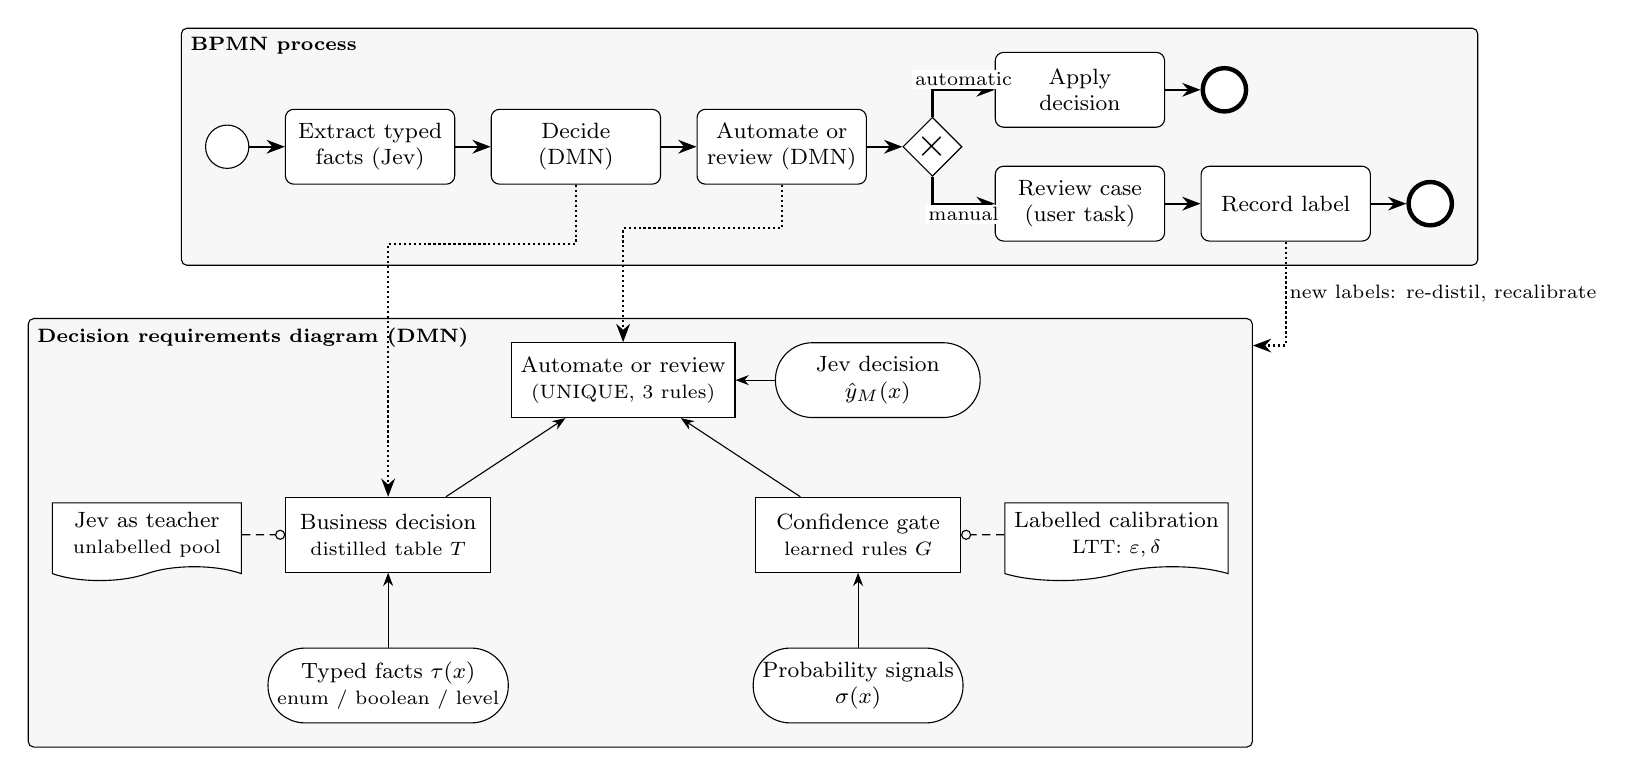
\begin{tikzpicture}[
    font=\footnotesize,
    >=Stealth,
    task/.style={draw, rounded corners=3pt, minimum width=2.15cm, minimum height=0.95cm, align=center, fill=white},
    event/.style={draw, circle, minimum size=0.55cm, fill=white},
    endevent/.style={draw, circle, line width=1.6pt, minimum size=0.55cm, fill=white},
    gateway/.style={draw, diamond, aspect=1, minimum size=0.75cm, inner sep=0pt, fill=white},
    decision/.style={draw, minimum width=2.6cm, minimum height=0.95cm, align=center, fill=white},
    input/.style={draw, rounded corners=0.47cm, minimum width=2.6cm, minimum height=0.95cm, align=center, fill=white},
    source/.style={draw, tape, tape bend top=none, minimum width=2.4cm, minimum height=0.95cm, align=center, fill=white},
    flow/.style={->, thick},
    req/.style={->, thin},
    auth/.style={-{Circle[open]}, densely dashed, thin},
    lbl/.style={font=\scriptsize, fill=white, inner sep=1pt},
  ]
  % ---------------- BPMN ----------------
  \node[event] (start) at (0,0) {};
  \node[task, right=0.45cm of start] (extract) {Extract typed\\facts (Jev)};
  \node[task, right=0.45cm of extract] (decide) {Decide\\(DMN)};
  \node[task, right=0.45cm of decide] (route) {Automate or\\review (DMN)};
  \node[gateway, right=0.45cm of route] (gw) {\Large$\times$};
  \node[task, above right=0.05cm and 0.6cm of gw] (apply) {Apply\\decision};
  \node[task, below right=0.05cm and 0.6cm of gw] (review) {Review case\\(user task)};
  \node[endevent, right=0.45cm of apply] (endA) {};
  \node[task, right=0.45cm of review] (record) {Record label};
  \node[endevent, right=0.45cm of record] (endB) {};
  \draw[flow] (start) -- (extract);
  \draw[flow] (extract) -- (decide);
  \draw[flow] (decide) -- (route);
  \draw[flow] (route) -- (gw);
  \draw[flow] (gw) |- node[lbl, pos=0.75, above] {automatic} (apply);
  \draw[flow] (gw) |- node[lbl, pos=0.75, below] {manual} (review);
  \draw[flow] (apply) -- (endA);
  \draw[flow] (review) -- (record);
  \draw[flow] (record) -- (endB);
  \begin{scope}[on background layer]
    \node[draw, fill=black!3, rounded corners=2pt, inner sep=0.3cm,
          fit=(start) (extract) (decide) (route) (gw) (apply) (review) (endA) (record) (endB),
          label={[anchor=north west, font=\scriptsize\bfseries]north west:BPMN process}] (bpmn) {};
  \end{scope}

  % ---------------- DRD ----------------
  \node[decision, below=2.0cm of decide, xshift=0.6cm] (outcome) {Automate or review\\{\scriptsize(UNIQUE, 3 rules)}};
  \node[decision, below left=1.0cm and 0.25cm of outcome] (business) {Business decision\\{\scriptsize distilled table $T$}};
  \node[decision, below right=1.0cm and 0.25cm of outcome] (gate) {Confidence gate\\{\scriptsize learned rules $G$}};
  \node[input, below=0.95cm of business] (facts) {Typed facts $\tau(x)$\\{\scriptsize enum / boolean / level}};
  \node[input, below=0.95cm of gate] (signals) {Probability signals\\$\sigma(x)$};
  \node[input, right=0.5cm of outcome] (holistic) {Jev decision\\$\hat y_{M}(x)$};
  \node[source, left=0.55cm of business] (teacher) {Jev as teacher\\{\scriptsize unlabelled pool}};
  \node[source, right=0.55cm of gate] (calib) {Labelled calibration\\{\scriptsize LTT: $\varepsilon,\delta$}};
  \draw[req] (facts) -- (business);
  \draw[req] (signals) -- (gate);
  \draw[req] (business) -- (outcome);
  \draw[req] (gate) -- (outcome);
  \draw[req] (holistic) -- (outcome);
  \draw[auth] (teacher) -- (business);
  \draw[auth] (calib) -- (gate);
  \begin{scope}[on background layer]
    \node[draw, fill=black!3, rounded corners=2pt, inner sep=0.3cm,
          fit=(outcome) (business) (gate) (facts) (signals) (holistic) (teacher) (calib),
          label={[anchor=north west, font=\scriptsize\bfseries]north west:Decision requirements diagram (DMN)}] (drd) {};
  \end{scope}
  \draw[->, densely dotted, thick] (decide.south) -- ++(0,-0.75) -| (business.north);
  \draw[->, densely dotted, thick] (route.south) -- ++(0,-0.55) -| (outcome.north);
  \draw[->, densely dotted, thick] (record.south) |- node[lbl, pos=0.25, right] {new labels: re-distil, recalibrate} ([yshift=-0.35cm]drd.north east);
\end{tikzpicture}
}
  \caption{Architecture. The BPMN process calls the System One model once per case and then evaluates a decision requirements diagram with three decisions. The business decision table is distilled from the model's own decisions (knowledge source on the left); the confidence gate is learned and thresholded on a labelled calibration set (knowledge source on the right). Cases decided by a reviewer produce labels for re-distillation and recalibration.}
  \label{fig:architecture}
\end{figure}

\begin{table}[pos=tbp]
  \centering
  \caption{Mapping of System One answer types to DMN. $p$ denotes the probability of the most likely answer; $n$ the number of options; $m^\star$ the most likely score level and $\bar d$ the mean absolute deviation of a uniform distribution over the levels.}
  \label{tab:types}
  \small
  \begin{tabular}{@{}llllp{4.3cm}@{}}
    \toprule
    Question & Model output & Typed value $\tau_j(x)$ & DMN type & Signals in $\sigma(x)$ \\
    \midrule
    Choice & distribution over $n\le 255$ options & most likely option & string, enumerated & $p$, confidence $\frac{p-1/n}{1-1/n}$, margin to 2nd \\
    Noul & probability of ``true'' & $p \ge 0.5$ & boolean & $p$, confidence $|2p-1|$ \\
    Score & distribution over $L\le 10$ levels & level $m^\star$ & number in $\{0,\dots,L-1\}$ & $p$, confidence $1-\frac{\sum_\ell \pi_\ell |\ell-m^\star|}{\bar d}$, margin \\
    \bottomrule
  \end{tabular}
\end{table}

Table~\ref{tab:types} gives the mapping from answers to DMN inputs. The typed value $\tau_j(x)$ is the most likely answer; together the typed values form the vector $\tau(x)\in D=D_1\times\dots\times D_m$. The signals $\sigma(x)$ summarise how certain each answer is; the confidence formulas are those of the vendor \citep{typesafe2026docs}. The model's holistic decision is $\hat y_M(x)=\arg\max_{c\in C}\pi_h(x)_c$ and the ground-truth decision, where available, is $y(x)$.

\subsection{Distilling the business decision table}\label{sec:distil}
The aim is a table $T: D\to C$ that reproduces $\hat y_M$ as closely as possible with as few rules as possible. Its \emph{fidelity} is $F(T)=\Pr[T(\tau(x))=\hat y_M(x)]$. Distillation needs no ground-truth labels: a pool $U$ of unlabelled cases is sent to $M$ once, and the pairs $(\tau(x),\hat y_M(x))$, $x\in U$, are the training data. Algorithm~\ref{alg:distil} summarises the procedure.

\begin{algorithm}[tbp]
  \caption{Distillation of a DMN decision table from a System One model.}
  \label{alg:distil}
  \small
  \KwIn{pool $U$; schema $(q_1,\dots,q_m,h)$; grids of depths and minimum leaf sizes; tolerance $t$}
  \KwOut{decision table $T$ with hit policy UNIQUE}
  Query $M$ once per $x\in U$; obtain $\tau(x)$ and $\hat y_M(x)$\;
  Encode $\tau(x)$: one-hot for choices, $0/1$ for nouls, integer level for scores\;
  Split $U$ into $U_{\mathrm{fit}}$ (80\%) and $U_{\mathrm{val}}$ (20\%)\;
  \ForEach{configuration $(d,\ell)$ in the grid}{
    Fit a CART tree of depth $\le d$ and leaf size $\ge \ell$ on $U_{\mathrm{fit}}$ with target $\hat y_M$\;
    $T_{d,\ell}\leftarrow$ \textsc{Merge}(\textsc{Paths}(tree)); record $|T_{d,\ell}|$ and fidelity on $U_{\mathrm{val}}$\;
  }
  Select the configuration with the fewest rules among those within $t$ of the best validation fidelity\;
  Refit it on $U$; \Return $T\leftarrow$ \textsc{Merge}(\textsc{Paths}(tree)) without unused inputs\;
\end{algorithm}

\paragraph{From paths to rules.} \textsc{Paths} turns each root-to-leaf path into one rule. Every split refers to an encoded column, which is mapped back to a condition on the original typed input: a split on the one-hot column for option $o$ of choice $q_j$ yields $\tau_j\in\{o\}$ or $\tau_j\in D_j\setminus\{o\}$; a split on a noul yields \feel{true} or \feel{false}; a split on a score yields a range of levels. Conditions on the same input are intersected along the path, so each rule assigns to every input a set $S_j\subseteq D_j$, written in FEEL as a list of values, a negated list (\feel{not("a","b")}), a range or \feel{-} when $S_j=D_j$. The rule's output is the majority class of its leaf; its support and purity are kept as rule annotations. Because the leaves of a tree partition the encoded space and every element of $D$ has exactly one encoding, the resulting rules partition $D$:

\begin{lemma}\label{lem:partition}
The rules produced by \textsc{Paths} are pairwise disjoint and cover $D$. Hence the table satisfies the UNIQUE hit policy and has no gaps on the whole input domain, not only on the observed cases.
\end{lemma}

The same translation applies to the gate, whose inputs are real-valued probabilities. A split $v\le\theta$ found on training values separates the largest value $a\le\theta$ from the smallest value $b>\theta$; any threshold $c\in[a,b)$ induces the same partition of the training data. We therefore write the shortest decimal in $[a,b)$, so that the table shows \feel{>= 0.88} rather than \feel{> 0.87645}, without changing any decision on the data the gate was fitted on.

\paragraph{Merging.} Two rules with the same output whose conditions coincide on all inputs but one, $j$, are replaced by a single rule with condition $S_j\cup S'_j$ (for real inputs only when the two intervals are adjacent, so that every cell remains one interval). As the two rules are disjoint boxes that differ in one dimension, their union is again a box and the table's semantics is unchanged; this is the merge step of \citet{calvanese2018}. We repeat merging to a fixpoint, grouping rules by their output and the conditions on all other inputs so that each pass is linear in the number of rules. Inputs that are \feel{-} in every rule are removed. For comparison we also report the size of an equivalent table with hit policy FIRST, in which the rules of the most frequent output are replaced by a final catch-all rule.

\paragraph{Model selection.} Fidelity usually grows with the number of rules while readability falls. Rather than fixing a size, we sweep tree depth and minimum leaf size and select the smallest table whose validation fidelity is within $t=1$ percentage point of the best; the full fidelity--complexity curve is reported.

\subsection{Verification}\label{sec:verify}
Lemma~\ref{lem:partition} holds by construction, but the exported artefact must also be checked. We verify each table in four ways. First, we compute all pairs of overlapping rules and the uncovered part of $D$ with box algebra: a rule is a box $\prod_j S_j$, two rules overlap if their conditions intersect on every input, and gaps are obtained by subtracting each rule from $D$, where the difference of two boxes is a union of at most $m$ disjoint boxes \citep{calvanese2018}. Second, the DRD is serialised to DMN~1.3 XML and validated against the OMG XML schema. Third, the XML is parsed back and its FEEL entries are evaluated by our own interpreter on every case; the outputs must equal those of the fitted tree. Fourth, an independent engine evaluates the same file: the DMN is parsed with \texttt{dmn-moddle} and its expressions and unary tests are evaluated with the FEEL interpreter \texttt{feelin} from the bpmn.io tool chain \citep{feelin}. Agreement of the four is required before a model is deployed.

\subsection{Risk-controlled confidence gate}\label{sec:gate}
Let $c(x)=\mathbb{1}[T(\tau(x))=y(x)]$ indicate that the table decides case $x$ correctly and $a(x)=\mathbb{1}[T(\tau(x))=\hat y_M(x)]$ that the table agrees with the model's holistic answer. A gate is a score $s(x)$ together with a threshold $\lambda$; a case is automated when $\tilde s(x)\ge\lambda$, where $\tilde s(x)=s(x)$ if $a(x)=1$ and $-\infty$ otherwise, so that disagreement always leads to review. The quantity a process owner cares about is the \emph{selective risk}
\begin{equation}
  R(\lambda)=\Pr\big[c(x)=0 \,\big|\, \tilde s(x)\ge\lambda\big],
\end{equation}
the error rate among automated cases, and the \emph{coverage} $\Pr[\tilde s(x)\ge\lambda]$, the share of cases automated. Given a tolerated error rate $\varepsilon$ and a failure probability $\delta$, we want the largest coverage such that $R(\lambda)\le\varepsilon$ holds with probability at least $1-\delta$.

\paragraph{Scores.} We compare two scores. The first is the model's own confidence in its holistic answer, $s(x)=\max_c\pi_h(x)_c$. The second is a \emph{learned gate}: a shallow classification tree (depth $\le 3$, at least 40 cases per leaf) fitted on the signals $\sigma(x)$ of the holistic question and of the facts used by $T$, with target $c(x)$; its score is the leaf estimate of $\Pr[c(x)=1]$. Because the tree is shallow, its leaves translate into a handful of readable DMN rules such as \feel{relief\_holistic\_\_conf >= 0.88}.

\paragraph{Threshold.} The labelled calibration set is split at random into halves $A$ and $B$. Half $A$ is used to fit the learned gate and to fix an ordered list of candidate thresholds $\lambda_1>\lambda_2>\dots>\lambda_K$ (Algorithm~\ref{alg:ltt}); half $B$ is used only for testing. For each candidate, let $n_k$ be the number of cases in $B$ with $\tilde s\ge\lambda_k$ and $e_k$ the number of errors among them. The null hypothesis $H_k: R(\lambda_k)>\varepsilon$ is tested with the exact binomial p-value $p_k=\Pr[\mathrm{Bin}(n_k,\varepsilon)\le e_k]$, and the hypotheses are tested in order until the first non-rejection.

\begin{algorithm}[tbp]
  \caption{Gate threshold by Learn-then-Test with fixed-sequence testing.}
  \label{alg:ltt}
  \small
  \KwIn{scores and correctness on halves $A$ and $B$; risk level $\varepsilon$; failure probability $\delta$; $K_{\max}$}
  \KwOut{threshold $\hat\lambda$ (accept $\tilde s\ge\hat\lambda$)}
  $n_{\min}\leftarrow\lceil \log\delta / \log(1-\varepsilon)\rceil$ \tcp*{fewest cases that can reject}
  On $A$: order distinct finite scores decreasingly; start at the first $\lambda$ for which a binomial test on $A$ rejects $H$ with at least $n_{\min}|A|/|B|$ accepted cases (else at the first with that many cases); keep $K_{\max}$ evenly spaced thresholds $\lambda_1>\dots>\lambda_K$\;
  $\hat\lambda\leftarrow+\infty$\;
  \For{$k=1,\dots,K$}{
    On $B$: $n_k\leftarrow|\{\tilde s\ge\lambda_k\}|$, $e_k\leftarrow$ errors among them, $p_k\leftarrow F_{\mathrm{Bin}(n_k,\varepsilon)}(e_k)$\;
    \lIf{$p_k>\delta$}{\textbf{break}}
    $\hat\lambda\leftarrow\lambda_k$\;
  }
  \Return $\hat\lambda$\;
\end{algorithm}

\begin{proposition}\label{prop:ltt}
Assume that the cases of half $B$ and future cases are independent and identically distributed and independent of half $A$ and of the pool used to build $T$. Then the threshold $\hat\lambda$ of Algorithm~\ref{alg:ltt} satisfies $\Pr\big[R(\hat\lambda)\le\varepsilon\big]\ge 1-\delta$.
\end{proposition}

\begin{proof}[Proof sketch]
Conditional on $A$ and the pool, the table, the score and the candidate list are fixed, so the hypotheses $H_1,\dots,H_K$ are fixed. Conditional on $n_k$, the cases of $B$ with $\tilde s\ge\lambda_k$ are an i.i.d.\ sample from the distribution of cases given $\tilde s\ge\lambda_k$, hence $e_k\sim\mathrm{Bin}(n_k,R(\lambda_k))$ and, under $H_k$, $\Pr[p_k\le u\mid n_k]\le u$ for all $u$; the p-value is therefore valid also unconditionally. Fixed-sequence testing rejects a true null only if the first true null in the sequence is rejected, which happens with probability at most $\delta$ whatever the dependence among the p-values; it thus controls the family-wise error rate at $\delta$ \citep{angelopoulos2025ltt}. If $R(\hat\lambda)>\varepsilon$, the true null $H_{\hat k}$ has been rejected, so $\Pr[R(\hat\lambda)>\varepsilon]\le\delta$.
\end{proof}

The guarantee does not require the model's probabilities to be calibrated; calibration only affects how many cases can be automated. Choosing the start of the sequence on $A$ matters in practice: fixed-sequence testing stops at the first non-rejection, and a sequence that starts at a threshold accepting only a few cases would stop immediately. When no candidate is rejected, $\hat\lambda=+\infty$ and every case is reviewed, which is the safe default.

\paragraph{Gate and outcome tables.} The learned gate is translated with \textsc{Paths}; each leaf outputs \feel{"auto"} if its score is at least $\hat\lambda$ and \feel{"review"} otherwise, and the rules are merged. The outcome decision is a three-rule UNIQUE table with inputs \emph{gate} and the FEEL expression \feel{business\_decision = holistic\_decision}; it returns \feel{"automatic"} only for (\feel{"auto"}, \feel{true}).

\subsection{Deployment and maintenance}
The DRD of Figure~\ref{fig:architecture} is deployed together with a BPMN process for Camunda~8: a service task calls the model and writes typed facts, signals and the holistic answer into process variables, two business rule tasks call the business and outcome decisions, and an exclusive gateway routes the case. Two knowledge sources document where the rules come from (the model version and the pool size) and how the gate was calibrated ($\varepsilon$, $\delta$, size of the calibration set). Because a model alias may move to a new version, the request pins a versioned model identifier and the response's model field is logged with every decision. Decisions made by reviewers become labels; they are used to monitor the selective risk in production and to recalibrate the gate or re-distil the table when the model, the case mix or the policy changes.

%% =======================================================================================
\section{Experimental design}\label{sec:design}

\subsection{Case and data}\label{sec:data}
We use the CFPB Consumer Complaint Database \citep{cfpb2026}, in which companies record how they closed each complaint; its narratives have been analysed, for example, with topic models to support complaint handling \citep{bastani2019}. The CFPB stopped publishing complaint narratives on 14~September~2026 \citep{cfpbnarratives2026}; we therefore take narratives from a public mirror of the database with complaints up to 2~January~2025 \citep{heineman2025} and join them by complaint identifier with the official bulk snapshot of 6~October~2026, which supplies the final company response. Only \res{data.labelchanged} of the joined complaints changed their response between the two snapshots, mostly from ``In progress'' to a final response. We keep complaints received between 1~April~2023 and 31~December~2024 with a narrative of at least 30 words, a closed response and a product in one of the ten product categories listed in Table~\ref{tab:tasks}, and drop exact duplicates of normalised narratives, which are common among templated letters and would otherwise leak between splits. This leaves \res{data.corpus} complaints.

\begin{table}[pos=tbp]
  \centering
  \caption{Decision tasks. Ground truth is derived from fields recorded by the CFPB; the model sees only the narrative.}
  \label{tab:tasks}
  \small
  \begin{tabular}{@{}p{2.3cm}p{5.6cm}p{6.3cm}@{}}
    \toprule
    Task & Cases and classes & Ground truth \\
    \midrule
    Monetary relief & \res{data.reliefn} random complaints about checking or savings accounts, credit and prepaid cards and money transfers; classes \feel{relief}, \feel{no\_relief} (\res{data.reliefpos} relief) & company response ``Closed with monetary relief'' versus ``Closed with explanation'' or ``Closed with non-monetary relief'' \\
    \addlinespace
    Routing & \res{data.routingn} complaints, \num{1250} per queue; eight queues: credit reporting, debt collection, deposits, cards, payments, mortgage, consumer loans, fraud & product group selected by the consumer; complaints whose issue or sub-issue denotes fraud, identity theft or unauthorised activity go to the fraud queue (14 issue/sub-issue pairs, listed in the repository) \\
    \bottomrule
  \end{tabular}
\end{table}

From this corpus we draw two samples with a fixed seed (Table~\ref{tab:tasks}). The relief task is a real business decision taken by the company after handling the complaint; among the \res{data.banking} banking complaints of the corpus, \res{data.bankingrelief} were resolved with monetary relief. The routing task uses the consumer's own classification as a proxy for the correct handling queue, simulating an intake channel such as e-mail or a call centre where no category is selected; the fraud queue makes the routing depend on more than the product. The union of both samples has \res{data.sample} complaints with a median length of \res{data.wordsmedian} words (interquartile range \res{data.wordsiqr}); \res{data.truncated} narratives longer than 1{,}500 words are truncated. Each task is split, stratified by its ground truth, into a pool (60\%), a calibration set (20\%) and a test set (20\%): \res{data.reliefpool}/\res{data.reliefcalibration}/\res{data.relieftest} cases for relief and \res{data.routingpool}/\res{data.routingcalibration}/\res{data.routingtest} for routing. Ground truth of the pool is never used by the distilled table.

\subsection{Question schema}\label{sec:schema}
All questions of both tasks are asked in a single request per complaint, with the narrative as the state. The schema (Table~\ref{tab:schema}) has fourteen fact questions and two holistic questions. The facts describe the complaint, not the decision: what product it concerns, whether the consumer reports unauthorised activity, a loss of money, a refund request or a denied claim, and how much financial harm is described. Following the vendor's guidance \citep{typesafe2026jagged}, every question states one literal condition, avoids arithmetic and dates and adds an explicit ``other'' option where the answer may not exist. Neither holistic question mentions the facts, so that the distilled table has to discover how the model's holistic judgement relates to them.

\begin{table}[pos=tbp]
  \centering
  \caption{Question schema (abridged wording; full text in the repository). C = choice, N = noul, S = score.}
  \label{tab:schema}
  \footnotesize
  \begin{tabular}{@{}llp{11.6cm}@{}}
    \toprule
    Id & Type & Question \\
    \midrule
    \feel{product} & C (11) & Which financial product or service is the complaint mainly about? (ten products, ``other'') \\
    \feel{unauthorized} & N & A transaction, charge, withdrawal or account was made without the consumer's permission. \\
    \feel{identity\_theft} & N & The consumer is a victim of identity theft. \\
    \feel{scam} & N & A scammer tricked the consumer into sending money or giving account access. \\
    \feel{report\_dispute} & N & The consumer disputes information on their credit report. \\
    \feel{collector\_contact} & N & The consumer complains about contact from a debt collector. \\
    \feel{money\_lost} & N & The consumer lost money or was charged money they believe they should not have paid. \\
    \feel{fee\_or\_interest} & N & The complaint is about a fee, a penalty or an interest charge. \\
    \feel{refund\_requested} & N & The consumer asks for a refund, reimbursement, credit or return of money. \\
    \feel{prior\_contact} & N & The consumer contacted the company about the problem before complaining. \\
    \feel{company\_admitted} & N & The company admitted a mistake or promised to fix the problem. \\
    \feel{claim\_denied} & N & The company denied or rejected the consumer's dispute, claim or request. \\
    \feel{funds\_blocked} & N & The consumer cannot use their account or money because the company froze, held, restricted or closed it. \\
    \feel{harm} & S (4) & How much financial harm is described? (none; small; significant or ongoing; severe) \\
    \midrule
    \feel{relief\_holistic} & N & Based on the complaint, the company should refund or reimburse money to the consumer. \\
    \feel{queue\_holistic} & C (8) & Which team should handle this complaint? (eight queues with one-line descriptions) \\
    \bottomrule
  \end{tabular}
\end{table}

\subsection{Model and protocol}
We call \jev{} through the System One API with the pinned model \texttt{jev-1.13.0} (reported model: \res{relief.models}). Each complaint is sent once; the request, the raw response, the latency and the time stamp are stored, and all analyses read from this record. Decision trees use scikit-learn \citep{pedregosa2011} with depths $\{1,\dots,6,8,10,12,\text{unbounded}\}$ and minimum leaf sizes $\{5,20,50,100\}$. The gate is calibrated for $\varepsilon\in\{0.01,0.02,0.05,0.10\}$ with $\delta=0.05$; the gate exported to DMN uses $\varepsilon=0.05$.

\subsection{Baselines}
We compare the distilled table (\emph{Jev+DMN, distilled}; no ground-truth labels) with: the majority class; \jev{}'s holistic answer (\emph{Jev holistic}; no labels); a decision table learned with the same procedure on \jev{}'s typed facts but with ground-truth labels as target (\emph{Jev+DMN, supervised}); and a TF-IDF representation of the narrative (word uni- and bigrams) with logistic regression (\emph{TF-IDF+LR}), a strong supervised text classifier without auditable logic. The supervised baselines are trained on labelled subsets of the pool of $\{100, 250, 500, 1000, 2000\}$ cases (five random repetitions) and on the whole pool, which shows how many labels they need to match the label-free approach. For the gate we compare no gate, the agreement filter alone, \jev{}'s confidence and the learned gate, each with and without the agreement filter.

\subsection{Metrics and statistical analysis}
Fidelity is the agreement between the table and \jev{}'s holistic answer on the test set, with Cohen's $\kappa$ \citep{cohen1960} and a 95\% percentile-bootstrap interval (2{,}000 resamples). Accuracy and macro-averaged F1 are computed against the ground truth. Calibration is measured by the top-label ECE with 15 equal-width bins (and equal-mass bins), the maximum calibration error, the multi-class Brier score \citep{brier1950} and reliability diagrams; isotonic recalibration is fitted on the calibration set and evaluated on the test set. For the gate we report coverage and selective risk on the test set, the area under the risk--coverage curve (AURC), and an empirical check of Proposition~\ref{prop:ltt}: the calibration and test cases are pooled and repeatedly split at random into $A$, $B$ and an evaluation part (200 repetitions), and we count how often the selective risk on the evaluation part exceeds $\varepsilon$. Paired accuracy differences are tested with the exact McNemar test \citep{mcnemar1947}. Table complexity is the number of rules, the number of inputs and the mean number of non-trivial conditions per rule. Operational metrics are the model latency per case (median and 95th percentile), the time to evaluate the table, the cost per 1{,}000 cases at the published price of \$0.042 per million input tokens, and the number of cases per 1{,}000 sent to review.

\subsection{Implementation}
The method is implemented in Python. The DMN writer produces DMN~1.3 XML with diagram interchange information, so the models open in DMN modelling tools; the BPMN model uses Camunda~8 extensions. The code, the question schema, the identifiers of all sampled complaints with their splits, the generated DMN and BPMN models and the scripts that produce every number and figure of this paper are available in the repository (Section~\ref{sec:data-availability}).

%% =======================================================================================
\section{Results}\label{sec:results}
%% NOTE: every number below is generated from results/jev by scripts/make_paper_assets.py.
%% Interpretive sentences marked TODO are to be written once the Jev run is complete.

\subsection{RQ1: Fidelity and complexity of distilled tables}\label{sec:res-rq1}
Table~\ref{tab:distillation} summarises the distilled tables. For the relief decision the selected table has \res{relief.rules} rules over \res{relief.inputs} inputs and reproduces \jev{}'s holistic decision on \res{relief.fidelity} of the test cases (95\% CI \res{relief.fidelityci}; $\kappa=\res{relief.kappa}$). For routing it has \res{routing.rules} rules over \res{routing.inputs} inputs with a fidelity of \res{routing.fidelity} (95\% CI \res{routing.fidelityci}; $\kappa=\res{routing.kappa}$). Merging reduced the tables from \res{relief.rulesraw} and \res{routing.rulesraw} tree leaves; with a FIRST hit policy and a default rule they need \res{relief.rulesfirst} and \res{routing.rulesfirst} rules. All tables passed every verification step: no conflicting overlaps and no gaps (as Lemma~\ref{lem:partition} predicts), XSD-valid XML, and identical outputs of the tree, our FEEL interpreter and the independent engine on all cases (round-trip agreement \res{relief.roundtrip} and \res{routing.roundtrip}). Figure~\ref{fig:complexity} shows the fidelity--complexity trade-off over all configurations. Table~\ref{tab:rules} shows the relief table as it appears in the DMN model.
% TODO(after Jev run): interpret which facts the tables use and where fidelity saturates.

\begin{table}[pos=tbp]
  \centering
  \caption{Distilled business decision tables (test set). Fidelity is agreement with \jev{}'s holistic decision; overlaps/gaps after merging.}
  \label{tab:distillation}
  \small
  \gentable{tab_distillation}
\end{table}

\begin{figure}[pos=tbp]
  \centering
  \genfigure{fig_complexity}
  \caption{Fidelity to \jev{} against the number of rules for all configurations of the sweep, refitted on the pool and evaluated on the test set. The step line is the Pareto front; the diamond marks the selected table.}
  \label{fig:complexity}
\end{figure}

\begin{table}[pos=tbp]
  \centering
  \caption{Distilled decision table for monetary relief (inputs that are ``\feel{-}'' in every rule omitted; support = pool cases per rule).}
  \label{tab:rules}
  \footnotesize
  \gentable{tab_rules_relief}
\end{table}

\subsection{RQ2: Calibration}\label{sec:res-rq2}
Table~\ref{tab:calibration} and Figure~\ref{fig:reliability} report how well \jev{}'s holistic probabilities match the true outcomes. On the test set, \jev{}'s holistic answer is correct for \res{relief.accholistic} of relief cases at a mean confidence of \res{relief.meanconf} (ECE \res{relief.ece}, Brier \res{relief.brier}) and for \res{routing.accholistic} of routing cases at a mean confidence of \res{routing.meanconf} (ECE \res{routing.ece}, Brier \res{routing.brier}). Isotonic recalibration on the calibration set changes the ECE to \res{relief.eceiso} and \res{routing.eceiso}, respectively.
% TODO(after Jev run): over- or under-confidence; does the vendor's calibration claim transfer to these tasks?

\begin{table}[pos=tbp]
  \centering
  \caption{Calibration of \jev{}'s holistic answer against the ground truth (test set).}
  \label{tab:calibration}
  \small
  \gentable{tab_calibration}
\end{table}

\begin{figure}[pos=tbp]
  \centering
  \genfigure{fig_reliability}
  \caption{Reliability diagrams of \jev{}'s top-label confidence on the test set, raw and after isotonic recalibration (bins with at least 10 cases).}
  \label{fig:reliability}
\end{figure}

\subsection{RQ3: Automation under a risk constraint}\label{sec:res-rq3}
Table~\ref{tab:gate} reports, for each gate and risk level, the share of test cases decided automatically and the error rate among them; Figure~\ref{fig:riskcov} shows the full risk--coverage curves. The table agrees with \jev{}'s holistic answer on \res{relief.agreerate} of relief and \res{routing.agreerate} of routing test cases; when it agrees, it is correct on \res{relief.accagree} and \res{routing.accagree} of the cases, and when it disagrees on \res{relief.accdisagree} and \res{routing.accdisagree}. At $\varepsilon=0.05$, the learned gate with the agreement filter automates \res{relief.learnedA.5.cov} of relief cases with an error rate of \res{relief.learnedA.5.risk}, and \res{routing.learnedA.5.cov} of routing cases with an error rate of \res{routing.learnedA.5.risk}. The AURC of the learned gate is \res{relief.aurclearned} (relief) and \res{routing.aurclearned} (routing), against \res{relief.aurcconf} and \res{routing.aurcconf} for \jev{}'s confidence. In the repeated-splitting check, the selective risk exceeded $\varepsilon=0.05$ in \res{relief.violation5} (relief) and \res{routing.violation5} (routing) of the 200 repetitions, against the nominal $\delta=5\%$.
% TODO(after Jev run): interpret contrast between tasks; which signals does the learned gate use?

\begin{table}[pos=tbp]
  \centering
  \caption{Coverage (Cov., \% of test cases automated) and selective risk (Risk, \% errors among automated cases) of the confidence gates, $\delta=0.05$. ``--'' marks levels at which no threshold was certified and all cases go to review.}
  \label{tab:gate}
  \footnotesize
  \gentable{tab_gate}
\end{table}

\begin{figure}[pos=tbp]
  \centering
  \genfigure{fig_risk_coverage}
  \caption{Risk--coverage curves on the test set (agreement filter not applied), with the risk levels $\varepsilon$ used for calibration.}
  \label{fig:riskcov}
\end{figure}

\subsection{RQ4: Comparison with baselines and operational cost}\label{sec:res-rq4}
Table~\ref{tab:baselines} compares the approaches. Without any labels, the distilled table reaches an accuracy of \res{relief.accdmn} on relief and \res{routing.accdmn} on routing, against \res{relief.accjev} and \res{routing.accjev} for \jev{}'s holistic answer (exact McNemar test: $p=\res{relief.mcnemarp}$ and $p=\res{routing.mcnemarp}$). With all \res{relief.labelsfull} (relief) and \res{routing.labelsfull} (routing) pool labels, the supervised table reaches \res{relief.accsupfull} and \res{routing.accsupfull}, and TF-IDF+LR \res{relief.acctfidffull} and \res{routing.acctfidffull}. Figure~\ref{fig:learning} shows how the supervised baselines depend on the number of labels.

The model answered a request with all sixteen questions in a median of \res{relief.latmed}~ms (95th percentile \res{relief.latp95}~ms) at a mean of \res{relief.tokens} input tokens, which corresponds to \$\res{relief.cost} per 1{,}000 cases. Evaluating the distilled table took \res{relief.dmnus}~$\mu$s per case in our Python implementation. At $\varepsilon=0.05$ the relief process sends \res{relief.review} and the routing process \res{routing.review} of every 1{,}000 cases to review.
% TODO(after Jev run): option-order robustness (reversed choice options on a random subset of test cases).
% TODO(after LLM key): LLM baseline with structured output via system-one-adapter (same questions).

\begin{table}[pos=tbp]
  \centering
  \caption{Accuracy against ground truth on the test set. Labels = ground-truth labels used for training; supervised results with all pool labels.}
  \label{tab:baselines}
  \small
  \gentable{tab_baselines}
\end{table}

\begin{figure}[pos=tbp]
  \centering
  \genfigure{fig_learning}
  \caption{Test accuracy of supervised baselines against the number of training labels (mean $\pm$ standard deviation over five draws), compared with the two label-free approaches.}
  \label{fig:learning}
\end{figure}

%% =======================================================================================
\section{Discussion}\label{sec:discussion}

\subsection{Implications for research}
The method separates three concerns that black-box automation entangles: reading the case, deciding, and deciding whether to decide. Reading is delegated to a model with typed output; deciding is done by a table that a person can read and that an engine executes; whether to decide is governed by a second table whose threshold carries a statistical guarantee. Each part can be inspected and replaced independently. This extends decision discovery \citep{bazhenova2016,desmedt2019,etinger2019} from structured logs to unstructured input, and it turns the abstract idea of a concept bottleneck \citep{koh2020} into an artefact of an industry standard.

Distillation from a model with typed output avoids two problems of distilling from free-text LLM output. There is nothing to parse: every answer is a value of a declared type, so the student's inputs are well defined. And the teacher's labels come with probabilities, which a text-generating model provides only through token likelihoods or verbalised confidence \citep{kadavath2022,xiong2024}. Fidelity measures how much of the model's holistic judgement can be expressed through the chosen facts; low fidelity is itself informative, because it signals that the schema misses a factor the model uses.
% TODO(after Jev run): relate fidelity and accuracy findings to this argument.

The confidence gate uses calibration data only where it is needed. Proposition~\ref{prop:ltt} holds whether or not the model is calibrated, so a process owner can rely on the stated error bound even for a model whose calibration on the task is unknown. Calibration, which RQ2 measures, determines how many cases the bound allows to be automated.

\subsection{Implications for practice}
For organisations, the approach provides a path to automating decisions on unstructured input that fits existing governance. The decision logic lives in a DMN table that business analysts can review and change through the usual change process; the knowledge sources in the DRD document which model version and which calibration data the rules come from. A risk owner sets $\varepsilon$ per decision, as with the different thresholds for low- and high-stakes actions in the vendor's guidance \citep{typesafe2026docs}, and the gate shows the price of that choice in reviewer workload. Every automated decision can be explained by the rule that fired and the facts that matched, which supports the transparency and human-oversight obligations of the AI Act \citep{euaiact2024}. Because the model is called once per case and the table evaluation is negligible, the latency and the cost per case are those of a single model request.

\subsection{Limitations and threats to validity}
\emph{Construct validity.} The ground truth of the relief task is what companies did, not what they should have done; relief also depends on company policies and on facts not in the narrative. The routing ground truth is the consumer's own choice of product and issue, which is a proxy for the correct queue. Both are noisy and bound the achievable accuracy of every method.

\emph{Internal validity.} Splits are stratified and fixed by a seed, the pool's labels are never used by the distilled table, calibration and test sets are disjoint, and exact duplicate narratives are removed. Near-duplicates may remain. The schema was designed before the experiments and was not tuned on the test set; a different schema would lead to different tables, and schema design is part of the method rather than a free parameter.

\emph{External validity.} We study one domain, one language and one model. \jev{} is a commercial model in early access whose weights are not available, so its results cannot be reproduced bit for bit; we mitigate this by pinning the model version, storing every request and response, and releasing the complaint identifiers. The method only assumes typed questions with probability distributions over answers, so it applies to other models of the class. An open adapter that emulates the System One interface with LLMs \citep{systemoneadapter} makes a reproduction with open models possible, at different latency and cost. The narratives come from a public mirror because the CFPB withdrew them from its database; the identifiers and the mirror's checksums are released so that the sample can be reconstructed.

\emph{Statistical validity.} Proposition~\ref{prop:ltt} assumes that future cases are exchangeable with the calibration cases. Changes in the case mix, the company policy or the model version break this assumption and require recalibration, for which the process supplies the labels.

%% =======================================================================================
\section{Conclusion}\label{sec:conclusion}
We showed how a System One model, which answers typed questions with probability distributions, can be turned into an auditable decision service in DMN. The model teaches a decision table over its own typed answers, which is verified and executed by a standard engine, and its probabilities drive a confidence gate whose threshold bounds the error rate of automated cases with a chosen probability. On \res{data.sample} complaints from the CFPB and two complaint-handling decisions we measured the fidelity and size of the distilled tables, the calibration of the model, the share of cases that can be automated at a given risk, and the trade-offs against the model alone and against supervised alternatives.
% TODO(after Jev run): one-sentence summary of the main quantitative findings.
Future work will apply the method to processes with richer state, combine distillation with the labels that reviewers produce, and study how tables and gates should be maintained when the underlying model is updated.

%% =======================================================================================
\section*{CRediT authorship contribution statement}
\printcredits

\section*{Declaration of competing interest}
%% TODO(authors): confirm. Mention any relationship with TypeSafe AI (e.g., early-access credits).
The authors declare that they have no known competing financial interests or personal relationships that could have appeared to influence the work reported in this paper.

\section*{Declaration of generative AI and AI-assisted technologies in the manuscript preparation process}
During the preparation of this work the author(s) used Claude (Anthropic) to assist with software development and with drafting and editing the manuscript. After using this tool, the author(s) reviewed and edited the content as needed and take(s) full responsibility for the content of the published article.

\section*{Data availability}\label{sec:data-availability}
%% TODO(authors): insert repository URL and archive DOI (e.g., Zenodo) before submission.
Code, question schema, complaint identifiers with splits, generated DMN and BPMN models, raw model responses and analysis scripts will be made available at [repository URL]. The complaint data are public \citep{cfpb2026,heineman2025}.

\section*{Funding}
%% TODO(authors): funding statement.
This research did not receive any specific grant from funding agencies in the public, commercial, or not-for-profit sectors.

\bibliographystyle{cas-model2-names}
\bibliography{refs}

\end{document}
"
\documentclass[a4paper,fleqn]{cas-sc}

\usepackage[authoryear,longnamesfirst]{natbib}
\usepackage{amsmath,amssymb,amsthm}
\usepackage{booktabs,multirow,makecell}
\usepackage{graphicx}
\usepackage{xcolor}
\usepackage[ruled,linesnumbered,vlined]{algorithm2e}
\usepackage{tikz}
\usetikzlibrary{arrows.meta,positioning,shapes.geometric,shapes.symbols,fit,backgrounds,calc}
\usepackage{enumitem}
\usepackage{siunitx}

\newtheorem{proposition}{Proposition}
\newtheorem{lemma}{Lemma}
\theoremstyle{definition}
\newtheorem{definition}{Definition}

%% ---------------------------------------------------------------------------------------
%% Numbers produced by the experiment pipeline (scripts/make_paper_assets.py, data_stats.py).
%% Missing values are printed as red placeholders, so nothing is ever typed in by hand.
\providecommand{\gendir}{generated}
\newcommand{\tbd}[1]{\textcolor{red}{[\detokenize{#1}]}}
\newcommand{\res}[1]{\ifcsname res@#1\endcsname\csname res@#1\endcsname\else\tbd{#1}\fi}
\InputIfFileExists{generated/data_numbers.tex}{}{}
\InputIfFileExists{\gendir/numbers.tex}{}{}
\newcommand{\gentable}[1]{\IfFileExists{\gendir/#1.tex}{\input{\gendir/#1}}{\tbd{#1: pending Jev run}}}
\newcommand{\genfigure}[2][\textwidth]{\IfFileExists{\gendir/#2.pdf}{\includegraphics[width=#1]{\gendir/#2}}{\fbox{\parbox{0.9\textwidth}{\centering\tbd{#2: pending Jev run}}}}}
\ifdefined\SimulatedResults
  \AddToHook{shipout/background}{\put(0.5\paperwidth,-0.5\paperheight){\makebox(0,0){\rotatebox{45}{\fontsize{40}{40}\selectfont\color{red!25}SIMULATED -- LAYOUT ONLY}}}}
\fi

\newcommand{\feel}[1]{\texttt{#1}}
\newcommand{\jev}{Jev}

\begin{document}
\let\WriteBookmarks\relax
\def\floatpagepagefraction{1}
\def\textpagefraction{.001}

\shorttitle{Distilling typed probabilistic decisions into DMN}
\shortauthors{D. Etinger}

\title[mode=title]{From typed probabilistic answers to auditable decision tables: distilling a System One model into DMN with risk-controlled automation}

\author[1]{Darko Etinger}[orcid=0000-0003-4444-7202]
\cormark[1]
\ead{darko.etinger@unipu.hr}
\credit{Conceptualization, Methodology, Software, Investigation, Writing -- original draft, Writing -- review \& editing}

%% TODO(authors): confirm Nikola Tanković's CRediT roles (placeholder below).
\author[1]{Nikola Tankovi\'c}[orcid=0000-0003-3936-1244]
\ead{nikola.tankovic@unipu.hr}
\credit{Writing -- review \& editing}

\affiliation[1]{organization={Juraj Dobrila University of Pula, Faculty of Informatics},
  addressline={Zagreba\v{c}ka 30},
  postcode={52100},
  city={Pula},
  country={Croatia}}

\cortext[1]{Corresponding author}

\begin{abstract}
Operational decisions in business processes increasingly start from unstructured input, such as complaints, e-mails or claims, that rule-based decision models cannot read. Language models can read such input, but their decision logic cannot be audited, and it is unclear when their output may be acted on without a human. We study a new class of models, System One models, which answer a fixed set of typed questions (choices, yes/no statements, ordinal scores) with a probability distribution for each answer, and show how to turn such a model into an auditable and executable decision service based on the Decision Model and Notation (DMN) standard. The model serves twice: as a teacher, whose holistic decisions on unlabelled cases are distilled into a DMN decision table over its own typed answers, and as a source of uncertainty, whose probabilities feed a confidence gate. The table is verified for overlaps and gaps and checked against an independent FEEL engine. The gate is learned from a small labelled set, and its threshold is chosen with Learn-then-Test, so that the error rate of automatically decided cases stays below a chosen level with high probability. We evaluate the approach with Jev, a commercial System One model, on \res{data.sample} consumer complaints from the Consumer Financial Protection Bureau in two tasks: deciding monetary relief and routing complaints to handling queues. We report the fidelity and size of the distilled tables, the calibration of the model's probabilities, the share of cases that can be automated at error levels between 1\% and 10\%, and the accuracy, latency and cost of the approach against the model alone and against supervised baselines.
\end{abstract}

\begin{highlights}
\item A typed probabilistic model is distilled into a verified DMN decision table.
\item The model's probabilities drive a learned confidence gate expressed in DMN.
\item Learn-then-Test thresholds bound the error rate of automated cases.
\item Exported decision models are XSD-valid and agree with an independent FEEL engine.
\item Evaluated on 17,674 CFPB complaints in two complaint-handling decisions.
\end{highlights}

\begin{keywords}
Decision Model and Notation \sep
Business process management \sep
Knowledge distillation \sep
Selective classification \sep
Risk control \sep
Human-in-the-loop automation
\end{keywords}

\maketitle

%% =======================================================================================
\section{Introduction}\label{sec:intro}

Operational decisions, such as approving a refund, routing a request or escalating a claim, are where business processes create or destroy value at scale \citep{dumas2018}. The Decision Model and Notation (DMN) standard \citep{omg_dmn13} separates such decisions from process control flow and expresses them as decision tables whose rules business analysts can read, test and change, and which process engines execute directly \citep{hasic2018,figl2018}. Decision tables have a well-defined semantics, so overlapping and missing rules can be detected automatically \citep{calvanese2016,calvanese2018}. These properties make DMN attractive wherever decisions must be explained to customers, auditors or regulators. In the European Union, for example, high-risk AI systems must be transparent to their deployers and allow effective human oversight \citep{euaiact2024}.

Decision tables, however, can only read structured data. A growing share of process instances starts from unstructured input: a complaint narrative, an e-mail, a call transcript, a claim description. Machine learning, and recently large language models (LLMs), can read such input \citep{vidgof2023}, but they put the decision logic in a black box, and their confidence statements are often poorly calibrated \citep{guo2017,xiong2024}. Organisations therefore face a choice between models that read unstructured input but cannot be audited, and rules that can be audited but cannot read the input. Neither tells them when a decision may be taken without a human.

A new class of models changes the shape of this problem. \emph{System One models} \citep{typesafe2026docs} do not generate text. They receive a state, for example a complaint, and a set of typed questions, and return for every question a probability distribution over a predefined set of answers: an option of a \emph{choice}, a level of an ordinal \emph{score}, or the probability that a statement is true (a \emph{noul}). The first model of this class, \jev{}, evaluates all questions in parallel and, according to its vendor, is trained to return calibrated probabilities at a latency of tens to hundreds of milliseconds \citep{typesafe2026docs}. Two properties make such models a natural match for DMN. Their answers are typed values from finite domains, which correspond directly to DMN data types. And they attach a probability to every answer, which can serve as an input to decision logic.

Existing work leaves this match unused. Decision discovery derives DMN models from historical, structured process data \citep{bazhenova2016,desmedt2019,goossens2024,leewis2024}; our earlier work translated decision trees learned from such data into DMN tables \citep{etinger2019} and combined tree ensembles in a layered architecture that generates DMN models \citep{simic2020}. Text-based approaches extract decision models from textual descriptions of decision logic \citep{goossens2023}, or let LLMs write DMN tables from given business rules \citep{cherednichenko2025}. None of them uses a model with typed probabilistic output both as the source of the decision logic and as the source of the signal that decides when that logic may run unattended.

We propose a method that does both. The System One model plays two roles. As a \emph{teacher}, it answers a set of decomposed fact questions and one holistic decision question on a large pool of unlabelled cases; a decision tree learned on its typed fact answers, with its holistic decision as the target, is translated into a DMN decision table, simplified and verified. At run time the model is reduced to a feature extractor, and the decision itself is taken by the table, which can be read and audited. As a \emph{source of uncertainty}, the model's probabilities feed a confidence gate, itself a small DMN table, that decides whether a case is decided automatically or sent to a person. The gate's threshold is chosen on a small labelled calibration set with Learn-then-Test \citep{angelopoulos2025ltt}, which guarantees, with a chosen probability, that the error rate among automatically decided cases does not exceed a chosen level. Disagreement between the table and the model's holistic answer is used as an additional signal for review. The whole decision service is one decision requirements diagram that a BPMN process calls from a business rule task.

We address four research questions:
\begin{description}[leftmargin=1.2cm,labelwidth=1cm,font=\normalfont\bfseries]
  \item[RQ1] How faithfully does a DMN table distilled from the model's typed answers reproduce the model's decisions, and at what table complexity?
  \item[RQ2] How well calibrated are the model's probabilities with respect to the true outcomes, and does post-hoc recalibration help?
  \item[RQ3] What share of cases can be decided automatically while the error rate of automated cases is kept below a given level?
  \item[RQ4] How does the approach compare with the model alone and with supervised baselines in accuracy, latency and cost, and how many labels would the supervised alternatives need?
\end{description}

We answer them on \res{data.sample} complaints from the Consumer Financial Protection Bureau (CFPB) in two decisions: whether a banking complaint should be resolved with monetary relief, and to which of eight queues a complaint should be routed. The contributions of the paper are:
\begin{enumerate}[label=(\arabic*)]
  \item a distillation method that turns the typed answers and holistic decisions of a System One model into DMN decision tables that are complete and free of conflicts by construction and that are verified statically, by round trip and by an independent FEEL engine;
  \item a confidence-gate pattern for DMN in which the gate's rules are learned from the model's probabilities and its threshold carries a finite-sample guarantee on the error rate of automated cases;
  \item an independent evaluation of the calibration and decision quality of a commercial System One model on a business process decision, against supervised baselines and their labelling cost;
  \item an open implementation with executable DMN and BPMN models.
\end{enumerate}

Section~\ref{sec:related} reviews related work. Section~\ref{sec:method} presents the method, Section~\ref{sec:design} the experimental design and Section~\ref{sec:results} the results. Section~\ref{sec:discussion} discusses implications and limitations, and Section~\ref{sec:conclusion} concludes.

%% =======================================================================================
\section{Background and related work}\label{sec:related}

\subsection{DMN decision tables}
DMN defines decision requirements diagrams (DRDs), in which decisions depend on input data, other decisions and business knowledge models, and are governed by knowledge sources \citep{omg_dmn13}. The most common decision logic is the decision table: each rule is a row of input entries, unary tests written in the Friendly Enough Expression Language (FEEL), and an output entry. A hit policy determines the result when several rules match; under the \emph{unique} policy at most one rule may match any input. \citet{calvanese2016,calvanese2018} gave decision tables a formal semantics, interpreted rules as hyper-rectangles in the input space and derived algorithms that detect overlapping rules and gaps (inputs no rule covers) and that merge rules to simplify tables. \citet{hasic2018} formulated principles for integrating decision and process models, and \citet{figl2018} reviewed what is known about the understandability and use of DMN. We reuse the geometric view of \citet{calvanese2018} to verify the tables we generate.

\subsection{Discovering decision logic from data}
Decision mining derives the conditions at process branching points from event logs \citep{rozinat2006,deleoni2013}. Later work produces DMN models: from process models in which decision logic is hard-coded \citep{batoulis2015}, from event logs \citep{bazhenova2016}, holistically from process execution data \citep{desmedt2019}, and from object-centric process data \citep{goossens2024}. \citet{leewis2024} proposed a framework that organises the discovery of operational decisions from data. In our earlier work we translated scikit-learn decision trees learned on structured data into DMN tables \citep{etinger2019}, and proposed a layered ensemble of decision-tree classifiers, generated as DMN models, to control the bias--variance trade-off on socially sensitive decision tasks \citep{simic2020}. All of these approaches learn from structured attributes recorded in historical data, and their tables are only as good as the recorded labels.

Two lines of work start from text. \citet{goossens2023} extract DMN models from natural-language descriptions of decision logic with deep learning, and \citet{cherednichenko2025} let an LLM with retrieval write DMN tables from business rules. \citet{arco2021} use natural-language processing to help decision modelers identify the inputs, outputs and rules in such descriptions. All of these translate a description of the logic into a model; none derives the logic from case data. \citet{bork2023} argue for hybrid decision management that combines AI components with explicit decision models, and LLM-based generation of process models is surveyed by \citet{horner2026}. Our setting differs from all of these: the input of each case is unstructured text, the logic is learned from a model's decisions on cases, and the model's uncertainty becomes part of the decision model.

\subsection{Distillation and interpretable surrogates}
Knowledge distillation transfers the behaviour of a teacher model to a student \citep{hinton2015}. When the student is a decision tree, the result is an interpretable surrogate of a black-box model \citep{craven1996,bastani2017,frosst2017}; rule ensembles are an alternative \citep{friedman2008}. Surrogates are judged by their \emph{fidelity}, the agreement with the teacher, and by their complexity \citep{guidotti2018}. \citet{rudin2019} argues that in high-stakes settings the deployed model should itself be interpretable rather than explained after the fact, for example by local post-hoc explanations \citep{ribeiro2016}; see \citet{arrieta2020} for a broader review of explainable AI. Our design follows that advice: the distilled table is the deployed decision logic, not an explanation of it.

The student in our method does not see the raw text but the teacher's answers to human-readable questions. This is the structure of concept bottleneck models, in which a model first predicts human-interpretable concepts and a simple model maps concepts to the output \citep{koh2020}. Recent work builds such bottlenecks with language models. \citet{benara2024} represent a text by an LLM's answers to a set of yes/no questions and fit sparse linear models on these answers, \citet{sun2025} train concept bottleneck LLMs for text classification, and \citet{singh2023} use an LLM only during training to build fully transparent models such as linear models and trees over n-grams. Using a language model as an annotator to replace human labelling has been studied for text classification \citep{wang2021,gilardi2023}. We combine the two ideas: the System One model supplies both the concepts (typed facts) and the labels (holistic decisions), so no ground-truth labels are needed to build the table. Unlike the approaches above, the concepts arrive with probability distributions that a gate can use, and the student is a decision table in an industry standard rather than a linear layer.

\subsection{Calibration, selective prediction and risk control}
A model is calibrated when its predicted probabilities match observed frequencies. Calibration is assessed with the Brier score \citep{brier1950}, the expected calibration error (ECE) and reliability diagrams \citep{naeini2015,guo2017}, and can be improved post hoc, for example with isotonic regression \citep{zadrozny2002}. Whether LLMs know what they know has been studied for token probabilities and verbalised confidence \citep{kadavath2022,tian2023,xiong2024}; \citet{geng2024} survey confidence estimation and calibration for LLMs, and \citet{kapoor2024} show that prompting alone does not produce reliable uncertainty estimates, whereas fine-tuning on a small set of graded answers does; System One models are claimed to be trained for calibration directly \citep{typesafe2026docs}, which we test independently.

Selective prediction lets a classifier abstain. \citet{chow1970} characterised the optimal trade-off between error and rejection; \citet{geifman2017} gave a method to select a confidence threshold with a guaranteed bound on the selective risk. Learning to defer extends the idea to deferring to a human expert \citep{madras2018,mozannar2020,raghu2019}, and \citet{wen2025} survey when and how LLMs should abstain. Conformal prediction gives distribution-free guarantees from exchangeable calibration data \citep{vovk2022}; conformal risk control and Learn-then-Test (LTT) generalise these guarantees to arbitrary risks and to the choice of any finite set of parameters by multiple hypothesis testing \citep{angelopoulos2024crc,angelopoulos2025ltt}. For language models, \citet{quach2024} calibrate conformal sets of generated answers, and \citet{ren2023} use conformal prediction to decide when an LLM-based planner should ask a person for help, which is the role our gate plays in a business process. We use LTT with fixed-sequence testing because the parameter we tune, the gate threshold, has a natural order and the controlled quantity, the error rate among automated cases, is what a process owner can specify.

\subsection{System One models}
The term follows the distinction between fast, intuitive judgements (System~1) and slow, deliberate reasoning (System~2) \citep{kahneman2011}. A System One request contains a \emph{state} (text or JSON) and a map of questions. A \emph{choice} selects one of up to 255 options and returns a distribution over them; a \emph{score} rates the state on an ordered rubric of up to ten levels and returns a distribution over levels and its expected value; a \emph{noul} returns the probability that a statement is true. Every question is answered in isolation from the others, in parallel, and answers can only take the declared values. The model we use, \jev{}, reports a confidence for choices and scores that rescales the top probability (choices) or the spread around the mode (scores) to $[0,1]$ \citep{typesafe2026docs}. The vendor documents known failure modes, among them literal reading of questions, weak arithmetic and date handling, and a preference for the first option of a choice \citep{typesafe2026jagged}; our question design and a robustness check address these (Sections~\ref{sec:schema} and~\ref{sec:res-rq4}).

%% =======================================================================================
\section{Method}\label{sec:method}

\subsection{Overview and notation}
Figure~\ref{fig:architecture} shows the architecture. A case $x$, here a complaint narrative, enters a BPMN process. A service task sends $x$ to the System One model $M$ with a fixed schema of $m$ \emph{fact questions} $q_1,\dots,q_m$ and one \emph{holistic question} $h$ per decision. For each fact question $q_j$ with answer domain $D_j$, $M$ returns a distribution $\pi_j(x)$ over $D_j$; for $h$ it returns a distribution $\pi_h(x)$ over the decision classes $C$. A business rule task then evaluates a DRD with three decisions: a \emph{business decision} table $T$ over the typed facts, a \emph{confidence gate} $G$ over probability signals, and an \emph{outcome} decision that automates the case only if the gate accepts it and $T$ agrees with $M$'s holistic answer. Otherwise a user task asks a person to decide, and the person's decision is stored as a new label.

\begin{figure}[pos=tbp]
  \centering
  \resizebox{\textwidth}{!}{% Architecture: BPMN process (top) and the decision requirements diagram it calls (bottom).
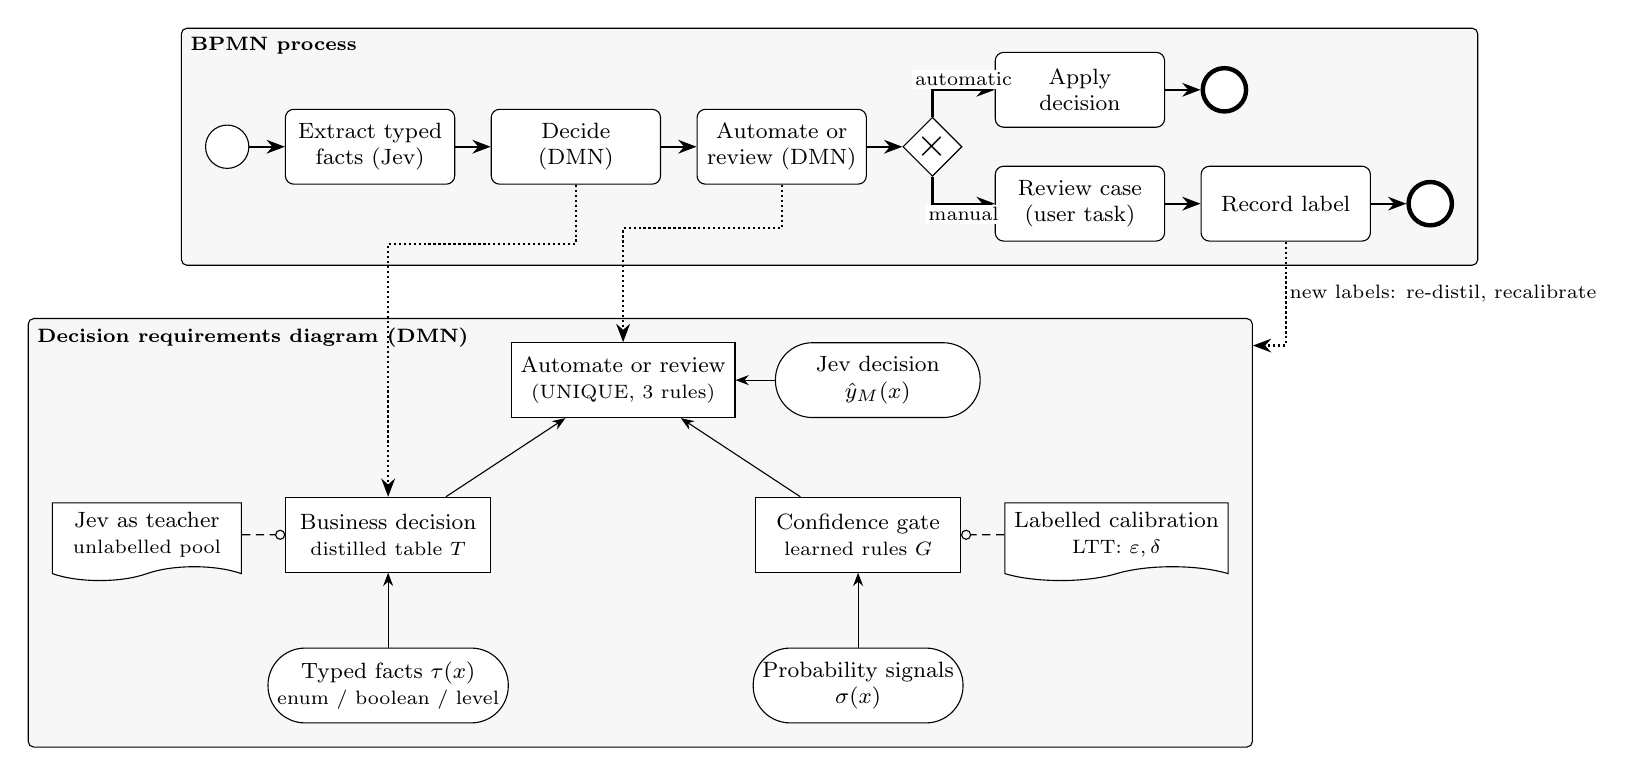
\begin{tikzpicture}[
    font=\footnotesize,
    >=Stealth,
    task/.style={draw, rounded corners=3pt, minimum width=2.15cm, minimum height=0.95cm, align=center, fill=white},
    event/.style={draw, circle, minimum size=0.55cm, fill=white},
    endevent/.style={draw, circle, line width=1.6pt, minimum size=0.55cm, fill=white},
    gateway/.style={draw, diamond, aspect=1, minimum size=0.75cm, inner sep=0pt, fill=white},
    decision/.style={draw, minimum width=2.6cm, minimum height=0.95cm, align=center, fill=white},
    input/.style={draw, rounded corners=0.47cm, minimum width=2.6cm, minimum height=0.95cm, align=center, fill=white},
    source/.style={draw, tape, tape bend top=none, minimum width=2.4cm, minimum height=0.95cm, align=center, fill=white},
    flow/.style={->, thick},
    req/.style={->, thin},
    auth/.style={-{Circle[open]}, densely dashed, thin},
    lbl/.style={font=\scriptsize, fill=white, inner sep=1pt},
  ]
  % ---------------- BPMN ----------------
  \node[event] (start) at (0,0) {};
  \node[task, right=0.45cm of start] (extract) {Extract typed\\facts (Jev)};
  \node[task, right=0.45cm of extract] (decide) {Decide\\(DMN)};
  \node[task, right=0.45cm of decide] (route) {Automate or\\review (DMN)};
  \node[gateway, right=0.45cm of route] (gw) {\Large$\times$};
  \node[task, above right=0.05cm and 0.6cm of gw] (apply) {Apply\\decision};
  \node[task, below right=0.05cm and 0.6cm of gw] (review) {Review case\\(user task)};
  \node[endevent, right=0.45cm of apply] (endA) {};
  \node[task, right=0.45cm of review] (record) {Record label};
  \node[endevent, right=0.45cm of record] (endB) {};
  \draw[flow] (start) -- (extract);
  \draw[flow] (extract) -- (decide);
  \draw[flow] (decide) -- (route);
  \draw[flow] (route) -- (gw);
  \draw[flow] (gw) |- node[lbl, pos=0.75, above] {automatic} (apply);
  \draw[flow] (gw) |- node[lbl, pos=0.75, below] {manual} (review);
  \draw[flow] (apply) -- (endA);
  \draw[flow] (review) -- (record);
  \draw[flow] (record) -- (endB);
  \begin{scope}[on background layer]
    \node[draw, fill=black!3, rounded corners=2pt, inner sep=0.3cm,
          fit=(start) (extract) (decide) (route) (gw) (apply) (review) (endA) (record) (endB),
          label={[anchor=north west, font=\scriptsize\bfseries]north west:BPMN process}] (bpmn) {};
  \end{scope}

  % ---------------- DRD ----------------
  \node[decision, below=2.0cm of decide, xshift=0.6cm] (outcome) {Automate or review\\{\scriptsize(UNIQUE, 3 rules)}};
  \node[decision, below left=1.0cm and 0.25cm of outcome] (business) {Business decision\\{\scriptsize distilled table $T$}};
  \node[decision, below right=1.0cm and 0.25cm of outcome] (gate) {Confidence gate\\{\scriptsize learned rules $G$}};
  \node[input, below=0.95cm of business] (facts) {Typed facts $\tau(x)$\\{\scriptsize enum / boolean / level}};
  \node[input, below=0.95cm of gate] (signals) {Probability signals\\$\sigma(x)$};
  \node[input, right=0.5cm of outcome] (holistic) {Jev decision\\$\hat y_{M}(x)$};
  \node[source, left=0.55cm of business] (teacher) {Jev as teacher\\{\scriptsize unlabelled pool}};
  \node[source, right=0.55cm of gate] (calib) {Labelled calibration\\{\scriptsize LTT: $\varepsilon,\delta$}};
  \draw[req] (facts) -- (business);
  \draw[req] (signals) -- (gate);
  \draw[req] (business) -- (outcome);
  \draw[req] (gate) -- (outcome);
  \draw[req] (holistic) -- (outcome);
  \draw[auth] (teacher) -- (business);
  \draw[auth] (calib) -- (gate);
  \begin{scope}[on background layer]
    \node[draw, fill=black!3, rounded corners=2pt, inner sep=0.3cm,
          fit=(outcome) (business) (gate) (facts) (signals) (holistic) (teacher) (calib),
          label={[anchor=north west, font=\scriptsize\bfseries]north west:Decision requirements diagram (DMN)}] (drd) {};
  \end{scope}
  \draw[->, densely dotted, thick] (decide.south) -- ++(0,-0.75) -| (business.north);
  \draw[->, densely dotted, thick] (route.south) -- ++(0,-0.55) -| (outcome.north);
  \draw[->, densely dotted, thick] (record.south) |- node[lbl, pos=0.25, right] {new labels: re-distil, recalibrate} ([yshift=-0.35cm]drd.north east);
\end{tikzpicture}
}
  \caption{Architecture. The BPMN process calls the System One model once per case and then evaluates a decision requirements diagram with three decisions. The business decision table is distilled from the model's own decisions (knowledge source on the left); the confidence gate is learned and thresholded on a labelled calibration set (knowledge source on the right). Cases decided by a reviewer produce labels for re-distillation and recalibration.}
  \label{fig:architecture}
\end{figure}

\begin{table}[pos=tbp]
  \centering
  \caption{Mapping of System One answer types to DMN. $p$ denotes the probability of the most likely answer; $n$ the number of options; $m^\star$ the most likely score level and $\bar d$ the mean absolute deviation of a uniform distribution over the levels.}
  \label{tab:types}
  \small
  \begin{tabular}{@{}llllp{4.3cm}@{}}
    \toprule
    Question & Model output & Typed value $\tau_j(x)$ & DMN type & Signals in $\sigma(x)$ \\
    \midrule
    Choice & distribution over $n\le 255$ options & most likely option & string, enumerated & $p$, confidence $\frac{p-1/n}{1-1/n}$, margin to 2nd \\
    Noul & probability of ``true'' & $p \ge 0.5$ & boolean & $p$, confidence $|2p-1|$ \\
    Score & distribution over $L\le 10$ levels & level $m^\star$ & number in $\{0,\dots,L-1\}$ & $p$, confidence $1-\frac{\sum_\ell \pi_\ell |\ell-m^\star|}{\bar d}$, margin \\
    \bottomrule
  \end{tabular}
\end{table}

Table~\ref{tab:types} gives the mapping from answers to DMN inputs. The typed value $\tau_j(x)$ is the most likely answer; together the typed values form the vector $\tau(x)\in D=D_1\times\dots\times D_m$. The signals $\sigma(x)$ summarise how certain each answer is; the confidence formulas are those of the vendor \citep{typesafe2026docs}. The model's holistic decision is $\hat y_M(x)=\arg\max_{c\in C}\pi_h(x)_c$ and the ground-truth decision, where available, is $y(x)$.

\subsection{Distilling the business decision table}\label{sec:distil}
The aim is a table $T: D\to C$ that reproduces $\hat y_M$ as closely as possible with as few rules as possible. Its \emph{fidelity} is $F(T)=\Pr[T(\tau(x))=\hat y_M(x)]$. Distillation needs no ground-truth labels: a pool $U$ of unlabelled cases is sent to $M$ once, and the pairs $(\tau(x),\hat y_M(x))$, $x\in U$, are the training data. Algorithm~\ref{alg:distil} summarises the procedure.

\begin{algorithm}[tbp]
  \caption{Distillation of a DMN decision table from a System One model.}
  \label{alg:distil}
  \small
  \KwIn{pool $U$; schema $(q_1,\dots,q_m,h)$; grids of depths and minimum leaf sizes; tolerance $t$}
  \KwOut{decision table $T$ with hit policy UNIQUE}
  Query $M$ once per $x\in U$; obtain $\tau(x)$ and $\hat y_M(x)$\;
  Encode $\tau(x)$: one-hot for choices, $0/1$ for nouls, integer level for scores\;
  Split $U$ into $U_{\mathrm{fit}}$ (80\%) and $U_{\mathrm{val}}$ (20\%)\;
  \ForEach{configuration $(d,\ell)$ in the grid}{
    Fit a CART tree of depth $\le d$ and leaf size $\ge \ell$ on $U_{\mathrm{fit}}$ with target $\hat y_M$\;
    $T_{d,\ell}\leftarrow$ \textsc{Merge}(\textsc{Paths}(tree)); record $|T_{d,\ell}|$ and fidelity on $U_{\mathrm{val}}$\;
  }
  Select the configuration with the fewest rules among those within $t$ of the best validation fidelity\;
  Refit it on $U$; \Return $T\leftarrow$ \textsc{Merge}(\textsc{Paths}(tree)) without unused inputs\;
\end{algorithm}

\paragraph{From paths to rules.} \textsc{Paths} turns each root-to-leaf path into one rule. Every split refers to an encoded column, which is mapped back to a condition on the original typed input: a split on the one-hot column for option $o$ of choice $q_j$ yields $\tau_j\in\{o\}$ or $\tau_j\in D_j\setminus\{o\}$; a split on a noul yields \feel{true} or \feel{false}; a split on a score yields a range of levels. Conditions on the same input are intersected along the path, so each rule assigns to every input a set $S_j\subseteq D_j$, written in FEEL as a list of values, a negated list (\feel{not("a","b")}), a range or \feel{-} when $S_j=D_j$. The rule's output is the majority class of its leaf; its support and purity are kept as rule annotations. Because the leaves of a tree partition the encoded space and every element of $D$ has exactly one encoding, the resulting rules partition $D$:

\begin{lemma}\label{lem:partition}
The rules produced by \textsc{Paths} are pairwise disjoint and cover $D$. Hence the table satisfies the UNIQUE hit policy and has no gaps on the whole input domain, not only on the observed cases.
\end{lemma}

The same translation applies to the gate, whose inputs are real-valued probabilities. A split $v\le\theta$ found on training values separates the largest value $a\le\theta$ from the smallest value $b>\theta$; any threshold $c\in[a,b)$ induces the same partition of the training data. We therefore write the shortest decimal in $[a,b)$, so that the table shows \feel{>= 0.88} rather than \feel{> 0.87645}, without changing any decision on the data the gate was fitted on.

\paragraph{Merging.} Two rules with the same output whose conditions coincide on all inputs but one, $j$, are replaced by a single rule with condition $S_j\cup S'_j$ (for real inputs only when the two intervals are adjacent, so that every cell remains one interval). As the two rules are disjoint boxes that differ in one dimension, their union is again a box and the table's semantics is unchanged; this is the merge step of \citet{calvanese2018}. We repeat merging to a fixpoint, grouping rules by their output and the conditions on all other inputs so that each pass is linear in the number of rules. Inputs that are \feel{-} in every rule are removed. For comparison we also report the size of an equivalent table with hit policy FIRST, in which the rules of the most frequent output are replaced by a final catch-all rule.

\paragraph{Model selection.} Fidelity usually grows with the number of rules while readability falls. Rather than fixing a size, we sweep tree depth and minimum leaf size and select the smallest table whose validation fidelity is within $t=1$ percentage point of the best; the full fidelity--complexity curve is reported.

\subsection{Verification}\label{sec:verify}
Lemma~\ref{lem:partition} holds by construction, but the exported artefact must also be checked. We verify each table in four ways. First, we compute all pairs of overlapping rules and the uncovered part of $D$ with box algebra: a rule is a box $\prod_j S_j$, two rules overlap if their conditions intersect on every input, and gaps are obtained by subtracting each rule from $D$, where the difference of two boxes is a union of at most $m$ disjoint boxes \citep{calvanese2018}. Second, the DRD is serialised to DMN~1.3 XML and validated against the OMG XML schema. Third, the XML is parsed back and its FEEL entries are evaluated by our own interpreter on every case; the outputs must equal those of the fitted tree. Fourth, an independent engine evaluates the same file: the DMN is parsed with \texttt{dmn-moddle} and its expressions and unary tests are evaluated with the FEEL interpreter \texttt{feelin} from the bpmn.io tool chain \citep{feelin}. Agreement of the four is required before a model is deployed.

\subsection{Risk-controlled confidence gate}\label{sec:gate}
Let $c(x)=\mathbb{1}[T(\tau(x))=y(x)]$ indicate that the table decides case $x$ correctly and $a(x)=\mathbb{1}[T(\tau(x))=\hat y_M(x)]$ that the table agrees with the model's holistic answer. A gate is a score $s(x)$ together with a threshold $\lambda$; a case is automated when $\tilde s(x)\ge\lambda$, where $\tilde s(x)=s(x)$ if $a(x)=1$ and $-\infty$ otherwise, so that disagreement always leads to review. The quantity a process owner cares about is the \emph{selective risk}
\begin{equation}
  R(\lambda)=\Pr\big[c(x)=0 \,\big|\, \tilde s(x)\ge\lambda\big],
\end{equation}
the error rate among automated cases, and the \emph{coverage} $\Pr[\tilde s(x)\ge\lambda]$, the share of cases automated. Given a tolerated error rate $\varepsilon$ and a failure probability $\delta$, we want the largest coverage such that $R(\lambda)\le\varepsilon$ holds with probability at least $1-\delta$.

\paragraph{Scores.} We compare two scores. The first is the model's own confidence in its holistic answer, $s(x)=\max_c\pi_h(x)_c$. The second is a \emph{learned gate}: a shallow classification tree (depth $\le 3$, at least 40 cases per leaf) fitted on the signals $\sigma(x)$ of the holistic question and of the facts used by $T$, with target $c(x)$; its score is the leaf estimate of $\Pr[c(x)=1]$. Because the tree is shallow, its leaves translate into a handful of readable DMN rules such as \feel{relief\_holistic\_\_conf >= 0.88}.

\paragraph{Threshold.} The labelled calibration set is split at random into halves $A$ and $B$. Half $A$ is used to fit the learned gate and to fix an ordered list of candidate thresholds $\lambda_1>\lambda_2>\dots>\lambda_K$ (Algorithm~\ref{alg:ltt}); half $B$ is used only for testing. For each candidate, let $n_k$ be the number of cases in $B$ with $\tilde s\ge\lambda_k$ and $e_k$ the number of errors among them. The null hypothesis $H_k: R(\lambda_k)>\varepsilon$ is tested with the exact binomial p-value $p_k=\Pr[\mathrm{Bin}(n_k,\varepsilon)\le e_k]$, and the hypotheses are tested in order until the first non-rejection.

\begin{algorithm}[tbp]
  \caption{Gate threshold by Learn-then-Test with fixed-sequence testing.}
  \label{alg:ltt}
  \small
  \KwIn{scores and correctness on halves $A$ and $B$; risk level $\varepsilon$; failure probability $\delta$; $K_{\max}$}
  \KwOut{threshold $\hat\lambda$ (accept $\tilde s\ge\hat\lambda$)}
  $n_{\min}\leftarrow\lceil \log\delta / \log(1-\varepsilon)\rceil$ \tcp*{fewest cases that can reject}
  On $A$: order distinct finite scores decreasingly; start at the first $\lambda$ for which a binomial test on $A$ rejects $H$ with at least $n_{\min}|A|/|B|$ accepted cases (else at the first with that many cases); keep $K_{\max}$ evenly spaced thresholds $\lambda_1>\dots>\lambda_K$\;
  $\hat\lambda\leftarrow+\infty$\;
  \For{$k=1,\dots,K$}{
    On $B$: $n_k\leftarrow|\{\tilde s\ge\lambda_k\}|$, $e_k\leftarrow$ errors among them, $p_k\leftarrow F_{\mathrm{Bin}(n_k,\varepsilon)}(e_k)$\;
    \lIf{$p_k>\delta$}{\textbf{break}}
    $\hat\lambda\leftarrow\lambda_k$\;
  }
  \Return $\hat\lambda$\;
\end{algorithm}

\begin{proposition}\label{prop:ltt}
Assume that the cases of half $B$ and future cases are independent and identically distributed and independent of half $A$ and of the pool used to build $T$. Then the threshold $\hat\lambda$ of Algorithm~\ref{alg:ltt} satisfies $\Pr\big[R(\hat\lambda)\le\varepsilon\big]\ge 1-\delta$.
\end{proposition}

\begin{proof}[Proof sketch]
Conditional on $A$ and the pool, the table, the score and the candidate list are fixed, so the hypotheses $H_1,\dots,H_K$ are fixed. Conditional on $n_k$, the cases of $B$ with $\tilde s\ge\lambda_k$ are an i.i.d.\ sample from the distribution of cases given $\tilde s\ge\lambda_k$, hence $e_k\sim\mathrm{Bin}(n_k,R(\lambda_k))$ and, under $H_k$, $\Pr[p_k\le u\mid n_k]\le u$ for all $u$; the p-value is therefore valid also unconditionally. Fixed-sequence testing rejects a true null only if the first true null in the sequence is rejected, which happens with probability at most $\delta$ whatever the dependence among the p-values; it thus controls the family-wise error rate at $\delta$ \citep{angelopoulos2025ltt}. If $R(\hat\lambda)>\varepsilon$, the true null $H_{\hat k}$ has been rejected, so $\Pr[R(\hat\lambda)>\varepsilon]\le\delta$.
\end{proof}

The guarantee does not require the model's probabilities to be calibrated; calibration only affects how many cases can be automated. Choosing the start of the sequence on $A$ matters in practice: fixed-sequence testing stops at the first non-rejection, and a sequence that starts at a threshold accepting only a few cases would stop immediately. When no candidate is rejected, $\hat\lambda=+\infty$ and every case is reviewed, which is the safe default.

\paragraph{Gate and outcome tables.} The learned gate is translated with \textsc{Paths}; each leaf outputs \feel{"auto"} if its score is at least $\hat\lambda$ and \feel{"review"} otherwise, and the rules are merged. The outcome decision is a three-rule UNIQUE table with inputs \emph{gate} and the FEEL expression \feel{business\_decision = holistic\_decision}; it returns \feel{"automatic"} only for (\feel{"auto"}, \feel{true}).

\subsection{Deployment and maintenance}
The DRD of Figure~\ref{fig:architecture} is deployed together with a BPMN process for Camunda~8: a service task calls the model and writes typed facts, signals and the holistic answer into process variables, two business rule tasks call the business and outcome decisions, and an exclusive gateway routes the case. Two knowledge sources document where the rules come from (the model version and the pool size) and how the gate was calibrated ($\varepsilon$, $\delta$, size of the calibration set). Because a model alias may move to a new version, the request pins a versioned model identifier and the response's model field is logged with every decision. Decisions made by reviewers become labels; they are used to monitor the selective risk in production and to recalibrate the gate or re-distil the table when the model, the case mix or the policy changes.

%% =======================================================================================
\section{Experimental design}\label{sec:design}

\subsection{Case and data}\label{sec:data}
We use the CFPB Consumer Complaint Database \citep{cfpb2026}, in which companies record how they closed each complaint; its narratives have been analysed, for example, with topic models to support complaint handling \citep{bastani2019}. The CFPB stopped publishing complaint narratives on 14~September~2026 \citep{cfpbnarratives2026}; we therefore take narratives from a public mirror of the database with complaints up to 2~January~2025 \citep{heineman2025} and join them by complaint identifier with the official bulk snapshot of 6~October~2026, which supplies the final company response. Only \res{data.labelchanged} of the joined complaints changed their response between the two snapshots, mostly from ``In progress'' to a final response. We keep complaints received between 1~April~2023 and 31~December~2024 with a narrative of at least 30 words, a closed response and a product in one of the ten product categories listed in Table~\ref{tab:tasks}, and drop exact duplicates of normalised narratives, which are common among templated letters and would otherwise leak between splits. This leaves \res{data.corpus} complaints.

\begin{table}[pos=tbp]
  \centering
  \caption{Decision tasks. Ground truth is derived from fields recorded by the CFPB; the model sees only the narrative.}
  \label{tab:tasks}
  \small
  \begin{tabular}{@{}p{2.3cm}p{5.6cm}p{6.3cm}@{}}
    \toprule
    Task & Cases and classes & Ground truth \\
    \midrule
    Monetary relief & \res{data.reliefn} random complaints about checking or savings accounts, credit and prepaid cards and money transfers; classes \feel{relief}, \feel{no\_relief} (\res{data.reliefpos} relief) & company response ``Closed with monetary relief'' versus ``Closed with explanation'' or ``Closed with non-monetary relief'' \\
    \addlinespace
    Routing & \res{data.routingn} complaints, \num{1250} per queue; eight queues: credit reporting, debt collection, deposits, cards, payments, mortgage, consumer loans, fraud & product group selected by the consumer; complaints whose issue or sub-issue denotes fraud, identity theft or unauthorised activity go to the fraud queue (14 issue/sub-issue pairs, listed in the repository) \\
    \bottomrule
  \end{tabular}
\end{table}

From this corpus we draw two samples with a fixed seed (Table~\ref{tab:tasks}). The relief task is a real business decision taken by the company after handling the complaint; among the \res{data.banking} banking complaints of the corpus, \res{data.bankingrelief} were resolved with monetary relief. The routing task uses the consumer's own classification as a proxy for the correct handling queue, simulating an intake channel such as e-mail or a call centre where no category is selected; the fraud queue makes the routing depend on more than the product. The union of both samples has \res{data.sample} complaints with a median length of \res{data.wordsmedian} words (interquartile range \res{data.wordsiqr}); \res{data.truncated} narratives longer than 1{,}500 words are truncated. Each task is split, stratified by its ground truth, into a pool (60\%), a calibration set (20\%) and a test set (20\%): \res{data.reliefpool}/\res{data.reliefcalibration}/\res{data.relieftest} cases for relief and \res{data.routingpool}/\res{data.routingcalibration}/\res{data.routingtest} for routing. Ground truth of the pool is never used by the distilled table.

\subsection{Question schema}\label{sec:schema}
All questions of both tasks are asked in a single request per complaint, with the narrative as the state. The schema (Table~\ref{tab:schema}) has fourteen fact questions and two holistic questions. The facts describe the complaint, not the decision: what product it concerns, whether the consumer reports unauthorised activity, a loss of money, a refund request or a denied claim, and how much financial harm is described. Following the vendor's guidance \citep{typesafe2026jagged}, every question states one literal condition, avoids arithmetic and dates and adds an explicit ``other'' option where the answer may not exist. Neither holistic question mentions the facts, so that the distilled table has to discover how the model's holistic judgement relates to them.

\begin{table}[pos=tbp]
  \centering
  \caption{Question schema (abridged wording; full text in the repository). C = choice, N = noul, S = score.}
  \label{tab:schema}
  \footnotesize
  \begin{tabular}{@{}llp{11.6cm}@{}}
    \toprule
    Id & Type & Question \\
    \midrule
    \feel{product} & C (11) & Which financial product or service is the complaint mainly about? (ten products, ``other'') \\
    \feel{unauthorized} & N & A transaction, charge, withdrawal or account was made without the consumer's permission. \\
    \feel{identity\_theft} & N & The consumer is a victim of identity theft. \\
    \feel{scam} & N & A scammer tricked the consumer into sending money or giving account access. \\
    \feel{report\_dispute} & N & The consumer disputes information on their credit report. \\
    \feel{collector\_contact} & N & The consumer complains about contact from a debt collector. \\
    \feel{money\_lost} & N & The consumer lost money or was charged money they believe they should not have paid. \\
    \feel{fee\_or\_interest} & N & The complaint is about a fee, a penalty or an interest charge. \\
    \feel{refund\_requested} & N & The consumer asks for a refund, reimbursement, credit or return of money. \\
    \feel{prior\_contact} & N & The consumer contacted the company about the problem before complaining. \\
    \feel{company\_admitted} & N & The company admitted a mistake or promised to fix the problem. \\
    \feel{claim\_denied} & N & The company denied or rejected the consumer's dispute, claim or request. \\
    \feel{funds\_blocked} & N & The consumer cannot use their account or money because the company froze, held, restricted or closed it. \\
    \feel{harm} & S (4) & How much financial harm is described? (none; small; significant or ongoing; severe) \\
    \midrule
    \feel{relief\_holistic} & N & Based on the complaint, the company should refund or reimburse money to the consumer. \\
    \feel{queue\_holistic} & C (8) & Which team should handle this complaint? (eight queues with one-line descriptions) \\
    \bottomrule
  \end{tabular}
\end{table}

\subsection{Model and protocol}
We call \jev{} through the System One API with the pinned model \texttt{jev-1.13.0} (reported model: \res{relief.models}). Each complaint is sent once; the request, the raw response, the latency and the time stamp are stored, and all analyses read from this record. Decision trees use scikit-learn \citep{pedregosa2011} with depths $\{1,\dots,6,8,10,12,\text{unbounded}\}$ and minimum leaf sizes $\{5,20,50,100\}$. The gate is calibrated for $\varepsilon\in\{0.01,0.02,0.05,0.10\}$ with $\delta=0.05$; the gate exported to DMN uses $\varepsilon=0.05$.

\subsection{Baselines}
We compare the distilled table (\emph{Jev+DMN, distilled}; no ground-truth labels) with: the majority class; \jev{}'s holistic answer (\emph{Jev holistic}; no labels); a decision table learned with the same procedure on \jev{}'s typed facts but with ground-truth labels as target (\emph{Jev+DMN, supervised}); and a TF-IDF representation of the narrative (word uni- and bigrams) with logistic regression (\emph{TF-IDF+LR}), a strong supervised text classifier without auditable logic. The supervised baselines are trained on labelled subsets of the pool of $\{100, 250, 500, 1000, 2000\}$ cases (five random repetitions) and on the whole pool, which shows how many labels they need to match the label-free approach. For the gate we compare no gate, the agreement filter alone, \jev{}'s confidence and the learned gate, each with and without the agreement filter.

\subsection{Metrics and statistical analysis}
Fidelity is the agreement between the table and \jev{}'s holistic answer on the test set, with Cohen's $\kappa$ \citep{cohen1960} and a 95\% percentile-bootstrap interval (2{,}000 resamples). Accuracy and macro-averaged F1 are computed against the ground truth. Calibration is measured by the top-label ECE with 15 equal-width bins (and equal-mass bins), the maximum calibration error, the multi-class Brier score \citep{brier1950} and reliability diagrams; isotonic recalibration is fitted on the calibration set and evaluated on the test set. For the gate we report coverage and selective risk on the test set, the area under the risk--coverage curve (AURC), and an empirical check of Proposition~\ref{prop:ltt}: the calibration and test cases are pooled and repeatedly split at random into $A$, $B$ and an evaluation part (200 repetitions), and we count how often the selective risk on the evaluation part exceeds $\varepsilon$. Paired accuracy differences are tested with the exact McNemar test \citep{mcnemar1947}. Table complexity is the number of rules, the number of inputs and the mean number of non-trivial conditions per rule. Operational metrics are the model latency per case (median and 95th percentile), the time to evaluate the table, the cost per 1{,}000 cases at the published price of \$0.042 per million input tokens, and the number of cases per 1{,}000 sent to review.

\subsection{Implementation}
The method is implemented in Python. The DMN writer produces DMN~1.3 XML with diagram interchange information, so the models open in DMN modelling tools; the BPMN model uses Camunda~8 extensions. The code, the question schema, the identifiers of all sampled complaints with their splits, the generated DMN and BPMN models and the scripts that produce every number and figure of this paper are available in the repository (Section~\ref{sec:data-availability}).

%% =======================================================================================
\section{Results}\label{sec:results}
%% NOTE: every number below is generated from results/jev by scripts/make_paper_assets.py.
%% Interpretive sentences marked TODO are to be written once the Jev run is complete.

\subsection{RQ1: Fidelity and complexity of distilled tables}\label{sec:res-rq1}
Table~\ref{tab:distillation} summarises the distilled tables. For the relief decision the selected table has \res{relief.rules} rules over \res{relief.inputs} inputs and reproduces \jev{}'s holistic decision on \res{relief.fidelity} of the test cases (95\% CI \res{relief.fidelityci}; $\kappa=\res{relief.kappa}$). For routing it has \res{routing.rules} rules over \res{routing.inputs} inputs with a fidelity of \res{routing.fidelity} (95\% CI \res{routing.fidelityci}; $\kappa=\res{routing.kappa}$). Merging reduced the tables from \res{relief.rulesraw} and \res{routing.rulesraw} tree leaves; with a FIRST hit policy and a default rule they need \res{relief.rulesfirst} and \res{routing.rulesfirst} rules. All tables passed every verification step: no conflicting overlaps and no gaps (as Lemma~\ref{lem:partition} predicts), XSD-valid XML, and identical outputs of the tree, our FEEL interpreter and the independent engine on all cases (round-trip agreement \res{relief.roundtrip} and \res{routing.roundtrip}). Figure~\ref{fig:complexity} shows the fidelity--complexity trade-off over all configurations. Table~\ref{tab:rules} shows the relief table as it appears in the DMN model.
% TODO(after Jev run): interpret which facts the tables use and where fidelity saturates.

\begin{table}[pos=tbp]
  \centering
  \caption{Distilled business decision tables (test set). Fidelity is agreement with \jev{}'s holistic decision; overlaps/gaps after merging.}
  \label{tab:distillation}
  \small
  \gentable{tab_distillation}
\end{table}

\begin{figure}[pos=tbp]
  \centering
  \genfigure{fig_complexity}
  \caption{Fidelity to \jev{} against the number of rules for all configurations of the sweep, refitted on the pool and evaluated on the test set. The step line is the Pareto front; the diamond marks the selected table.}
  \label{fig:complexity}
\end{figure}

\begin{table}[pos=tbp]
  \centering
  \caption{Distilled decision table for monetary relief (inputs that are ``\feel{-}'' in every rule omitted; support = pool cases per rule).}
  \label{tab:rules}
  \footnotesize
  \gentable{tab_rules_relief}
\end{table}

\subsection{RQ2: Calibration}\label{sec:res-rq2}
Table~\ref{tab:calibration} and Figure~\ref{fig:reliability} report how well \jev{}'s holistic probabilities match the true outcomes. On the test set, \jev{}'s holistic answer is correct for \res{relief.accholistic} of relief cases at a mean confidence of \res{relief.meanconf} (ECE \res{relief.ece}, Brier \res{relief.brier}) and for \res{routing.accholistic} of routing cases at a mean confidence of \res{routing.meanconf} (ECE \res{routing.ece}, Brier \res{routing.brier}). Isotonic recalibration on the calibration set changes the ECE to \res{relief.eceiso} and \res{routing.eceiso}, respectively.
% TODO(after Jev run): over- or under-confidence; does the vendor's calibration claim transfer to these tasks?

\begin{table}[pos=tbp]
  \centering
  \caption{Calibration of \jev{}'s holistic answer against the ground truth (test set).}
  \label{tab:calibration}
  \small
  \gentable{tab_calibration}
\end{table}

\begin{figure}[pos=tbp]
  \centering
  \genfigure{fig_reliability}
  \caption{Reliability diagrams of \jev{}'s top-label confidence on the test set, raw and after isotonic recalibration (bins with at least 10 cases).}
  \label{fig:reliability}
\end{figure}

\subsection{RQ3: Automation under a risk constraint}\label{sec:res-rq3}
Table~\ref{tab:gate} reports, for each gate and risk level, the share of test cases decided automatically and the error rate among them; Figure~\ref{fig:riskcov} shows the full risk--coverage curves. The table agrees with \jev{}'s holistic answer on \res{relief.agreerate} of relief and \res{routing.agreerate} of routing test cases; when it agrees, it is correct on \res{relief.accagree} and \res{routing.accagree} of the cases, and when it disagrees on \res{relief.accdisagree} and \res{routing.accdisagree}. At $\varepsilon=0.05$, the learned gate with the agreement filter automates \res{relief.learnedA.5.cov} of relief cases with an error rate of \res{relief.learnedA.5.risk}, and \res{routing.learnedA.5.cov} of routing cases with an error rate of \res{routing.learnedA.5.risk}. The AURC of the learned gate is \res{relief.aurclearned} (relief) and \res{routing.aurclearned} (routing), against \res{relief.aurcconf} and \res{routing.aurcconf} for \jev{}'s confidence. In the repeated-splitting check, the selective risk exceeded $\varepsilon=0.05$ in \res{relief.violation5} (relief) and \res{routing.violation5} (routing) of the 200 repetitions, against the nominal $\delta=5\%$.
% TODO(after Jev run): interpret contrast between tasks; which signals does the learned gate use?

\begin{table}[pos=tbp]
  \centering
  \caption{Coverage (Cov., \% of test cases automated) and selective risk (Risk, \% errors among automated cases) of the confidence gates, $\delta=0.05$. ``--'' marks levels at which no threshold was certified and all cases go to review.}
  \label{tab:gate}
  \footnotesize
  \gentable{tab_gate}
\end{table}

\begin{figure}[pos=tbp]
  \centering
  \genfigure{fig_risk_coverage}
  \caption{Risk--coverage curves on the test set (agreement filter not applied), with the risk levels $\varepsilon$ used for calibration.}
  \label{fig:riskcov}
\end{figure}

\subsection{RQ4: Comparison with baselines and operational cost}\label{sec:res-rq4}
Table~\ref{tab:baselines} compares the approaches. Without any labels, the distilled table reaches an accuracy of \res{relief.accdmn} on relief and \res{routing.accdmn} on routing, against \res{relief.accjev} and \res{routing.accjev} for \jev{}'s holistic answer (exact McNemar test: $p=\res{relief.mcnemarp}$ and $p=\res{routing.mcnemarp}$). With all \res{relief.labelsfull} (relief) and \res{routing.labelsfull} (routing) pool labels, the supervised table reaches \res{relief.accsupfull} and \res{routing.accsupfull}, and TF-IDF+LR \res{relief.acctfidffull} and \res{routing.acctfidffull}. Figure~\ref{fig:learning} shows how the supervised baselines depend on the number of labels.

The model answered a request with all sixteen questions in a median of \res{relief.latmed}~ms (95th percentile \res{relief.latp95}~ms) at a mean of \res{relief.tokens} input tokens, which corresponds to \$\res{relief.cost} per 1{,}000 cases. Evaluating the distilled table took \res{relief.dmnus}~$\mu$s per case in our Python implementation. At $\varepsilon=0.05$ the relief process sends \res{relief.review} and the routing process \res{routing.review} of every 1{,}000 cases to review.
% TODO(after Jev run): option-order robustness (reversed choice options on a random subset of test cases).
% TODO(after LLM key): LLM baseline with structured output via system-one-adapter (same questions).

\begin{table}[pos=tbp]
  \centering
  \caption{Accuracy against ground truth on the test set. Labels = ground-truth labels used for training; supervised results with all pool labels.}
  \label{tab:baselines}
  \small
  \gentable{tab_baselines}
\end{table}

\begin{figure}[pos=tbp]
  \centering
  \genfigure{fig_learning}
  \caption{Test accuracy of supervised baselines against the number of training labels (mean $\pm$ standard deviation over five draws), compared with the two label-free approaches.}
  \label{fig:learning}
\end{figure}

%% =======================================================================================
\section{Discussion}\label{sec:discussion}

\subsection{Implications for research}
The method separates three concerns that black-box automation entangles: reading the case, deciding, and deciding whether to decide. Reading is delegated to a model with typed output; deciding is done by a table that a person can read and that an engine executes; whether to decide is governed by a second table whose threshold carries a statistical guarantee. Each part can be inspected and replaced independently. This extends decision discovery \citep{bazhenova2016,desmedt2019,etinger2019} from structured logs to unstructured input, and it turns the abstract idea of a concept bottleneck \citep{koh2020} into an artefact of an industry standard.

Distillation from a model with typed output avoids two problems of distilling from free-text LLM output. There is nothing to parse: every answer is a value of a declared type, so the student's inputs are well defined. And the teacher's labels come with probabilities, which a text-generating model provides only through token likelihoods or verbalised confidence \citep{kadavath2022,xiong2024}. Fidelity measures how much of the model's holistic judgement can be expressed through the chosen facts; low fidelity is itself informative, because it signals that the schema misses a factor the model uses.
% TODO(after Jev run): relate fidelity and accuracy findings to this argument.

The confidence gate uses calibration data only where it is needed. Proposition~\ref{prop:ltt} holds whether or not the model is calibrated, so a process owner can rely on the stated error bound even for a model whose calibration on the task is unknown. Calibration, which RQ2 measures, determines how many cases the bound allows to be automated.

\subsection{Implications for practice}
For organisations, the approach provides a path to automating decisions on unstructured input that fits existing governance. The decision logic lives in a DMN table that business analysts can review and change through the usual change process; the knowledge sources in the DRD document which model version and which calibration data the rules come from. A risk owner sets $\varepsilon$ per decision, as with the different thresholds for low- and high-stakes actions in the vendor's guidance \citep{typesafe2026docs}, and the gate shows the price of that choice in reviewer workload. Every automated decision can be explained by the rule that fired and the facts that matched, which supports the transparency and human-oversight obligations of the AI Act \citep{euaiact2024}. Because the model is called once per case and the table evaluation is negligible, the latency and the cost per case are those of a single model request.

\subsection{Limitations and threats to validity}
\emph{Construct validity.} The ground truth of the relief task is what companies did, not what they should have done; relief also depends on company policies and on facts not in the narrative. The routing ground truth is the consumer's own choice of product and issue, which is a proxy for the correct queue. Both are noisy and bound the achievable accuracy of every method.

\emph{Internal validity.} Splits are stratified and fixed by a seed, the pool's labels are never used by the distilled table, calibration and test sets are disjoint, and exact duplicate narratives are removed. Near-duplicates may remain. The schema was designed before the experiments and was not tuned on the test set; a different schema would lead to different tables, and schema design is part of the method rather than a free parameter.

\emph{External validity.} We study one domain, one language and one model. \jev{} is a commercial model in early access whose weights are not available, so its results cannot be reproduced bit for bit; we mitigate this by pinning the model version, storing every request and response, and releasing the complaint identifiers. The method only assumes typed questions with probability distributions over answers, so it applies to other models of the class. An open adapter that emulates the System One interface with LLMs \citep{systemoneadapter} makes a reproduction with open models possible, at different latency and cost. The narratives come from a public mirror because the CFPB withdrew them from its database; the identifiers and the mirror's checksums are released so that the sample can be reconstructed.

\emph{Statistical validity.} Proposition~\ref{prop:ltt} assumes that future cases are exchangeable with the calibration cases. Changes in the case mix, the company policy or the model version break this assumption and require recalibration, for which the process supplies the labels.

%% =======================================================================================
\section{Conclusion}\label{sec:conclusion}
We showed how a System One model, which answers typed questions with probability distributions, can be turned into an auditable decision service in DMN. The model teaches a decision table over its own typed answers, which is verified and executed by a standard engine, and its probabilities drive a confidence gate whose threshold bounds the error rate of automated cases with a chosen probability. On \res{data.sample} complaints from the CFPB and two complaint-handling decisions we measured the fidelity and size of the distilled tables, the calibration of the model, the share of cases that can be automated at a given risk, and the trade-offs against the model alone and against supervised alternatives.
% TODO(after Jev run): one-sentence summary of the main quantitative findings.
Future work will apply the method to processes with richer state, combine distillation with the labels that reviewers produce, and study how tables and gates should be maintained when the underlying model is updated.

%% =======================================================================================
\section*{CRediT authorship contribution statement}
\printcredits

\section*{Declaration of competing interest}
%% TODO(authors): confirm. Mention any relationship with TypeSafe AI (e.g., early-access credits).
The authors declare that they have no known competing financial interests or personal relationships that could have appeared to influence the work reported in this paper.

\section*{Declaration of generative AI and AI-assisted technologies in the manuscript preparation process}
During the preparation of this work the author(s) used Claude (Anthropic) to assist with software development and with drafting and editing the manuscript. After using this tool, the author(s) reviewed and edited the content as needed and take(s) full responsibility for the content of the published article.

\section*{Data availability}\label{sec:data-availability}
%% TODO(authors): insert repository URL and archive DOI (e.g., Zenodo) before submission.
Code, question schema, complaint identifiers with splits, generated DMN and BPMN models, raw model responses and analysis scripts will be made available at [repository URL]. The complaint data are public \citep{cfpb2026,heineman2025}.

\section*{Funding}
%% TODO(authors): funding statement.
This research did not receive any specific grant from funding agencies in the public, commercial, or not-for-profit sectors.

\bibliographystyle{cas-model2-names}
\bibliography{refs}

\end{document}
"
\documentclass[a4paper,fleqn]{cas-sc}

\usepackage[authoryear,longnamesfirst]{natbib}
\usepackage{amsmath,amssymb,amsthm}
\usepackage{booktabs,multirow,makecell}
\usepackage{graphicx}
\usepackage{xcolor}
\usepackage[ruled,linesnumbered,vlined]{algorithm2e}
\usepackage{tikz}
\usetikzlibrary{arrows.meta,positioning,shapes.geometric,shapes.symbols,fit,backgrounds,calc}
\usepackage{enumitem}
\usepackage{siunitx}

\newtheorem{proposition}{Proposition}
\newtheorem{lemma}{Lemma}
\theoremstyle{definition}
\newtheorem{definition}{Definition}

%% ---------------------------------------------------------------------------------------
%% Numbers produced by the experiment pipeline (scripts/make_paper_assets.py, data_stats.py).
%% Missing values are printed as red placeholders, so nothing is ever typed in by hand.
\providecommand{\gendir}{generated}
\newcommand{\tbd}[1]{\textcolor{red}{[\detokenize{#1}]}}
\newcommand{\res}[1]{\ifcsname res@#1\endcsname\csname res@#1\endcsname\else\tbd{#1}\fi}
\InputIfFileExists{generated/data_numbers.tex}{}{}
\InputIfFileExists{\gendir/numbers.tex}{}{}
\newcommand{\gentable}[1]{\IfFileExists{\gendir/#1.tex}{\input{\gendir/#1}}{\tbd{#1: pending Jev run}}}
\newcommand{\genfigure}[2][\textwidth]{\IfFileExists{\gendir/#2.pdf}{\includegraphics[width=#1]{\gendir/#2}}{\fbox{\parbox{0.9\textwidth}{\centering\tbd{#2: pending Jev run}}}}}
\ifdefined\SimulatedResults
  \AddToHook{shipout/background}{\put(0.5\paperwidth,-0.5\paperheight){\makebox(0,0){\rotatebox{45}{\fontsize{40}{40}\selectfont\color{red!25}SIMULATED -- LAYOUT ONLY}}}}
\fi

\newcommand{\feel}[1]{\texttt{#1}}
\newcommand{\jev}{Jev}

\begin{document}
\let\WriteBookmarks\relax
\def\floatpagepagefraction{1}
\def\textpagefraction{.001}

\shorttitle{Distilling typed probabilistic decisions into DMN}
\shortauthors{D. Etinger}

\title[mode=title]{From typed probabilistic answers to auditable decision tables: distilling a System One model into DMN with risk-controlled automation}

\author[1]{Darko Etinger}[orcid=0000-0003-4444-7202]
\cormark[1]
\ead{darko.etinger@unipu.hr}
\credit{Conceptualization, Methodology, Software, Investigation, Writing -- original draft, Writing -- review \& editing}

%% TODO(authors): confirm Nikola Tanković's CRediT roles (placeholder below).
\author[1]{Nikola Tankovi\'c}[orcid=0000-0003-3936-1244]
\ead{nikola.tankovic@unipu.hr}
\credit{Writing -- review \& editing}

\affiliation[1]{organization={Juraj Dobrila University of Pula, Faculty of Informatics},
  addressline={Zagreba\v{c}ka 30},
  postcode={52100},
  city={Pula},
  country={Croatia}}

\cortext[1]{Corresponding author}

\begin{abstract}
Operational decisions in business processes increasingly start from unstructured input, such as complaints, e-mails or claims, that rule-based decision models cannot read. Language models can read such input, but their decision logic cannot be audited, and it is unclear when their output may be acted on without a human. We study a new class of models, System One models, which answer a fixed set of typed questions (choices, yes/no statements, ordinal scores) with a probability distribution for each answer, and show how to turn such a model into an auditable and executable decision service based on the Decision Model and Notation (DMN) standard. The model serves twice: as a teacher, whose holistic decisions on unlabelled cases are distilled into a DMN decision table over its own typed answers, and as a source of uncertainty, whose probabilities feed a confidence gate. The table is verified for overlaps and gaps and checked against an independent FEEL engine. The gate is learned from a small labelled set, and its threshold is chosen with Learn-then-Test, so that the error rate of automatically decided cases stays below a chosen level with high probability. We evaluate the approach with Jev, a commercial System One model, on \res{data.sample} consumer complaints from the Consumer Financial Protection Bureau in two tasks: deciding monetary relief and routing complaints to handling queues. We report the fidelity and size of the distilled tables, the calibration of the model's probabilities, the share of cases that can be automated at error levels between 1\% and 10\%, and the accuracy, latency and cost of the approach against the model alone and against supervised baselines.
\end{abstract}

\begin{highlights}
\item A typed probabilistic model is distilled into a verified DMN decision table.
\item The model's probabilities drive a learned confidence gate expressed in DMN.
\item Learn-then-Test thresholds bound the error rate of automated cases.
\item Exported decision models are XSD-valid and agree with an independent FEEL engine.
\item Evaluated on 17,674 CFPB complaints in two complaint-handling decisions.
\end{highlights}

\begin{keywords}
Decision Model and Notation \sep
Business process management \sep
Knowledge distillation \sep
Selective classification \sep
Risk control \sep
Human-in-the-loop automation
\end{keywords}

\maketitle

%% =======================================================================================
\section{Introduction}\label{sec:intro}

Operational decisions, such as approving a refund, routing a request or escalating a claim, are where business processes create or destroy value at scale \citep{dumas2018}. The Decision Model and Notation (DMN) standard \citep{omg_dmn13} separates such decisions from process control flow and expresses them as decision tables whose rules business analysts can read, test and change, and which process engines execute directly \citep{hasic2018,figl2018}. Decision tables have a well-defined semantics, so overlapping and missing rules can be detected automatically \citep{calvanese2016,calvanese2018}. These properties make DMN attractive wherever decisions must be explained to customers, auditors or regulators. In the European Union, for example, high-risk AI systems must be transparent to their deployers and allow effective human oversight \citep{euaiact2024}.

Decision tables, however, can only read structured data. A growing share of process instances starts from unstructured input: a complaint narrative, an e-mail, a call transcript, a claim description. Machine learning, and recently large language models (LLMs), can read such input \citep{vidgof2023}, but they put the decision logic in a black box, and their confidence statements are often poorly calibrated \citep{guo2017,xiong2024}. Organisations therefore face a choice between models that read unstructured input but cannot be audited, and rules that can be audited but cannot read the input. Neither tells them when a decision may be taken without a human.

A new class of models changes the shape of this problem. \emph{System One models} \citep{typesafe2026docs} do not generate text. They receive a state, for example a complaint, and a set of typed questions, and return for every question a probability distribution over a predefined set of answers: an option of a \emph{choice}, a level of an ordinal \emph{score}, or the probability that a statement is true (a \emph{noul}). The first model of this class, \jev{}, evaluates all questions in parallel and, according to its vendor, is trained to return calibrated probabilities at a latency of tens to hundreds of milliseconds \citep{typesafe2026docs}. Two properties make such models a natural match for DMN. Their answers are typed values from finite domains, which correspond directly to DMN data types. And they attach a probability to every answer, which can serve as an input to decision logic.

Existing work leaves this match unused. Decision discovery derives DMN models from historical, structured process data \citep{bazhenova2016,desmedt2019,goossens2024,leewis2024}; our earlier work translated decision trees learned from such data into DMN tables \citep{etinger2019} and combined tree ensembles in a layered architecture that generates DMN models \citep{simic2020}. Text-based approaches extract decision models from textual descriptions of decision logic \citep{goossens2023}, or let LLMs write DMN tables from given business rules \citep{cherednichenko2025}. None of them uses a model with typed probabilistic output both as the source of the decision logic and as the source of the signal that decides when that logic may run unattended.

We propose a method that does both. The System One model plays two roles. As a \emph{teacher}, it answers a set of decomposed fact questions and one holistic decision question on a large pool of unlabelled cases; a decision tree learned on its typed fact answers, with its holistic decision as the target, is translated into a DMN decision table, simplified and verified. At run time the model is reduced to a feature extractor, and the decision itself is taken by the table, which can be read and audited. As a \emph{source of uncertainty}, the model's probabilities feed a confidence gate, itself a small DMN table, that decides whether a case is decided automatically or sent to a person. The gate's threshold is chosen on a small labelled calibration set with Learn-then-Test \citep{angelopoulos2025ltt}, which guarantees, with a chosen probability, that the error rate among automatically decided cases does not exceed a chosen level. Disagreement between the table and the model's holistic answer is used as an additional signal for review. The whole decision service is one decision requirements diagram that a BPMN process calls from a business rule task.

We address four research questions:
\begin{description}[leftmargin=1.2cm,labelwidth=1cm,font=\normalfont\bfseries]
  \item[RQ1] How faithfully does a DMN table distilled from the model's typed answers reproduce the model's decisions, and at what table complexity?
  \item[RQ2] How well calibrated are the model's probabilities with respect to the true outcomes, and does post-hoc recalibration help?
  \item[RQ3] What share of cases can be decided automatically while the error rate of automated cases is kept below a given level?
  \item[RQ4] How does the approach compare with the model alone and with supervised baselines in accuracy, latency and cost, and how many labels would the supervised alternatives need?
\end{description}

We answer them on \res{data.sample} complaints from the Consumer Financial Protection Bureau (CFPB) in two decisions: whether a banking complaint should be resolved with monetary relief, and to which of eight queues a complaint should be routed. The contributions of the paper are:
\begin{enumerate}[label=(\arabic*)]
  \item a distillation method that turns the typed answers and holistic decisions of a System One model into DMN decision tables that are complete and free of conflicts by construction and that are verified statically, by round trip and by an independent FEEL engine;
  \item a confidence-gate pattern for DMN in which the gate's rules are learned from the model's probabilities and its threshold carries a finite-sample guarantee on the error rate of automated cases;
  \item an independent evaluation of the calibration and decision quality of a commercial System One model on a business process decision, against supervised baselines and their labelling cost;
  \item an open implementation with executable DMN and BPMN models.
\end{enumerate}

Section~\ref{sec:related} reviews related work. Section~\ref{sec:method} presents the method, Section~\ref{sec:design} the experimental design and Section~\ref{sec:results} the results. Section~\ref{sec:discussion} discusses implications and limitations, and Section~\ref{sec:conclusion} concludes.

%% =======================================================================================
\section{Background and related work}\label{sec:related}

\subsection{DMN decision tables}
DMN defines decision requirements diagrams (DRDs), in which decisions depend on input data, other decisions and business knowledge models, and are governed by knowledge sources \citep{omg_dmn13}. The most common decision logic is the decision table: each rule is a row of input entries, unary tests written in the Friendly Enough Expression Language (FEEL), and an output entry. A hit policy determines the result when several rules match; under the \emph{unique} policy at most one rule may match any input. \citet{calvanese2016,calvanese2018} gave decision tables a formal semantics, interpreted rules as hyper-rectangles in the input space and derived algorithms that detect overlapping rules and gaps (inputs no rule covers) and that merge rules to simplify tables. \citet{hasic2018} formulated principles for integrating decision and process models, and \citet{figl2018} reviewed what is known about the understandability and use of DMN. We reuse the geometric view of \citet{calvanese2018} to verify the tables we generate.

\subsection{Discovering decision logic from data}
Decision mining derives the conditions at process branching points from event logs \citep{rozinat2006,deleoni2013}. Later work produces DMN models: from process models in which decision logic is hard-coded \citep{batoulis2015}, from event logs \citep{bazhenova2016}, holistically from process execution data \citep{desmedt2019}, and from object-centric process data \citep{goossens2024}. \citet{leewis2024} proposed a framework that organises the discovery of operational decisions from data. In our earlier work we translated scikit-learn decision trees learned on structured data into DMN tables \citep{etinger2019}, and proposed a layered ensemble of decision-tree classifiers, generated as DMN models, to control the bias--variance trade-off on socially sensitive decision tasks \citep{simic2020}. All of these approaches learn from structured attributes recorded in historical data, and their tables are only as good as the recorded labels.

Two lines of work start from text. \citet{goossens2023} extract DMN models from natural-language descriptions of decision logic with deep learning, and \citet{cherednichenko2025} let an LLM with retrieval write DMN tables from business rules. \citet{arco2021} use natural-language processing to help decision modelers identify the inputs, outputs and rules in such descriptions. All of these translate a description of the logic into a model; none derives the logic from case data. \citet{bork2023} argue for hybrid decision management that combines AI components with explicit decision models, and LLM-based generation of process models is surveyed by \citet{horner2026}. Our setting differs from all of these: the input of each case is unstructured text, the logic is learned from a model's decisions on cases, and the model's uncertainty becomes part of the decision model.

\subsection{Distillation and interpretable surrogates}
Knowledge distillation transfers the behaviour of a teacher model to a student \citep{hinton2015}. When the student is a decision tree, the result is an interpretable surrogate of a black-box model \citep{craven1996,bastani2017,frosst2017}; rule ensembles are an alternative \citep{friedman2008}. Surrogates are judged by their \emph{fidelity}, the agreement with the teacher, and by their complexity \citep{guidotti2018}. \citet{rudin2019} argues that in high-stakes settings the deployed model should itself be interpretable rather than explained after the fact, for example by local post-hoc explanations \citep{ribeiro2016}; see \citet{arrieta2020} for a broader review of explainable AI. Our design follows that advice: the distilled table is the deployed decision logic, not an explanation of it.

The student in our method does not see the raw text but the teacher's answers to human-readable questions. This is the structure of concept bottleneck models, in which a model first predicts human-interpretable concepts and a simple model maps concepts to the output \citep{koh2020}. Recent work builds such bottlenecks with language models. \citet{benara2024} represent a text by an LLM's answers to a set of yes/no questions and fit sparse linear models on these answers, \citet{sun2025} train concept bottleneck LLMs for text classification, and \citet{singh2023} use an LLM only during training to build fully transparent models such as linear models and trees over n-grams. Using a language model as an annotator to replace human labelling has been studied for text classification \citep{wang2021,gilardi2023}. We combine the two ideas: the System One model supplies both the concepts (typed facts) and the labels (holistic decisions), so no ground-truth labels are needed to build the table. Unlike the approaches above, the concepts arrive with probability distributions that a gate can use, and the student is a decision table in an industry standard rather than a linear layer.

\subsection{Calibration, selective prediction and risk control}
A model is calibrated when its predicted probabilities match observed frequencies. Calibration is assessed with the Brier score \citep{brier1950}, the expected calibration error (ECE) and reliability diagrams \citep{naeini2015,guo2017}, and can be improved post hoc, for example with isotonic regression \citep{zadrozny2002}. Whether LLMs know what they know has been studied for token probabilities and verbalised confidence \citep{kadavath2022,tian2023,xiong2024}; \citet{geng2024} survey confidence estimation and calibration for LLMs, and \citet{kapoor2024} show that prompting alone does not produce reliable uncertainty estimates, whereas fine-tuning on a small set of graded answers does; System One models are claimed to be trained for calibration directly \citep{typesafe2026docs}, which we test independently.

Selective prediction lets a classifier abstain. \citet{chow1970} characterised the optimal trade-off between error and rejection; \citet{geifman2017} gave a method to select a confidence threshold with a guaranteed bound on the selective risk. Learning to defer extends the idea to deferring to a human expert \citep{madras2018,mozannar2020,raghu2019}, and \citet{wen2025} survey when and how LLMs should abstain. Conformal prediction gives distribution-free guarantees from exchangeable calibration data \citep{vovk2022}; conformal risk control and Learn-then-Test (LTT) generalise these guarantees to arbitrary risks and to the choice of any finite set of parameters by multiple hypothesis testing \citep{angelopoulos2024crc,angelopoulos2025ltt}. For language models, \citet{quach2024} calibrate conformal sets of generated answers, and \citet{ren2023} use conformal prediction to decide when an LLM-based planner should ask a person for help, which is the role our gate plays in a business process. We use LTT with fixed-sequence testing because the parameter we tune, the gate threshold, has a natural order and the controlled quantity, the error rate among automated cases, is what a process owner can specify.

\subsection{System One models}
The term follows the distinction between fast, intuitive judgements (System~1) and slow, deliberate reasoning (System~2) \citep{kahneman2011}. A System One request contains a \emph{state} (text or JSON) and a map of questions. A \emph{choice} selects one of up to 255 options and returns a distribution over them; a \emph{score} rates the state on an ordered rubric of up to ten levels and returns a distribution over levels and its expected value; a \emph{noul} returns the probability that a statement is true. Every question is answered in isolation from the others, in parallel, and answers can only take the declared values. The model we use, \jev{}, reports a confidence for choices and scores that rescales the top probability (choices) or the spread around the mode (scores) to $[0,1]$ \citep{typesafe2026docs}. The vendor documents known failure modes, among them literal reading of questions, weak arithmetic and date handling, and a preference for the first option of a choice \citep{typesafe2026jagged}; our question design and a robustness check address these (Sections~\ref{sec:schema} and~\ref{sec:res-rq4}).

%% =======================================================================================
\section{Method}\label{sec:method}

\subsection{Overview and notation}
Figure~\ref{fig:architecture} shows the architecture. A case $x$, here a complaint narrative, enters a BPMN process. A service task sends $x$ to the System One model $M$ with a fixed schema of $m$ \emph{fact questions} $q_1,\dots,q_m$ and one \emph{holistic question} $h$ per decision. For each fact question $q_j$ with answer domain $D_j$, $M$ returns a distribution $\pi_j(x)$ over $D_j$; for $h$ it returns a distribution $\pi_h(x)$ over the decision classes $C$. A business rule task then evaluates a DRD with three decisions: a \emph{business decision} table $T$ over the typed facts, a \emph{confidence gate} $G$ over probability signals, and an \emph{outcome} decision that automates the case only if the gate accepts it and $T$ agrees with $M$'s holistic answer. Otherwise a user task asks a person to decide, and the person's decision is stored as a new label.

\begin{figure}[pos=tbp]
  \centering
  \resizebox{\textwidth}{!}{% Architecture: BPMN process (top) and the decision requirements diagram it calls (bottom).
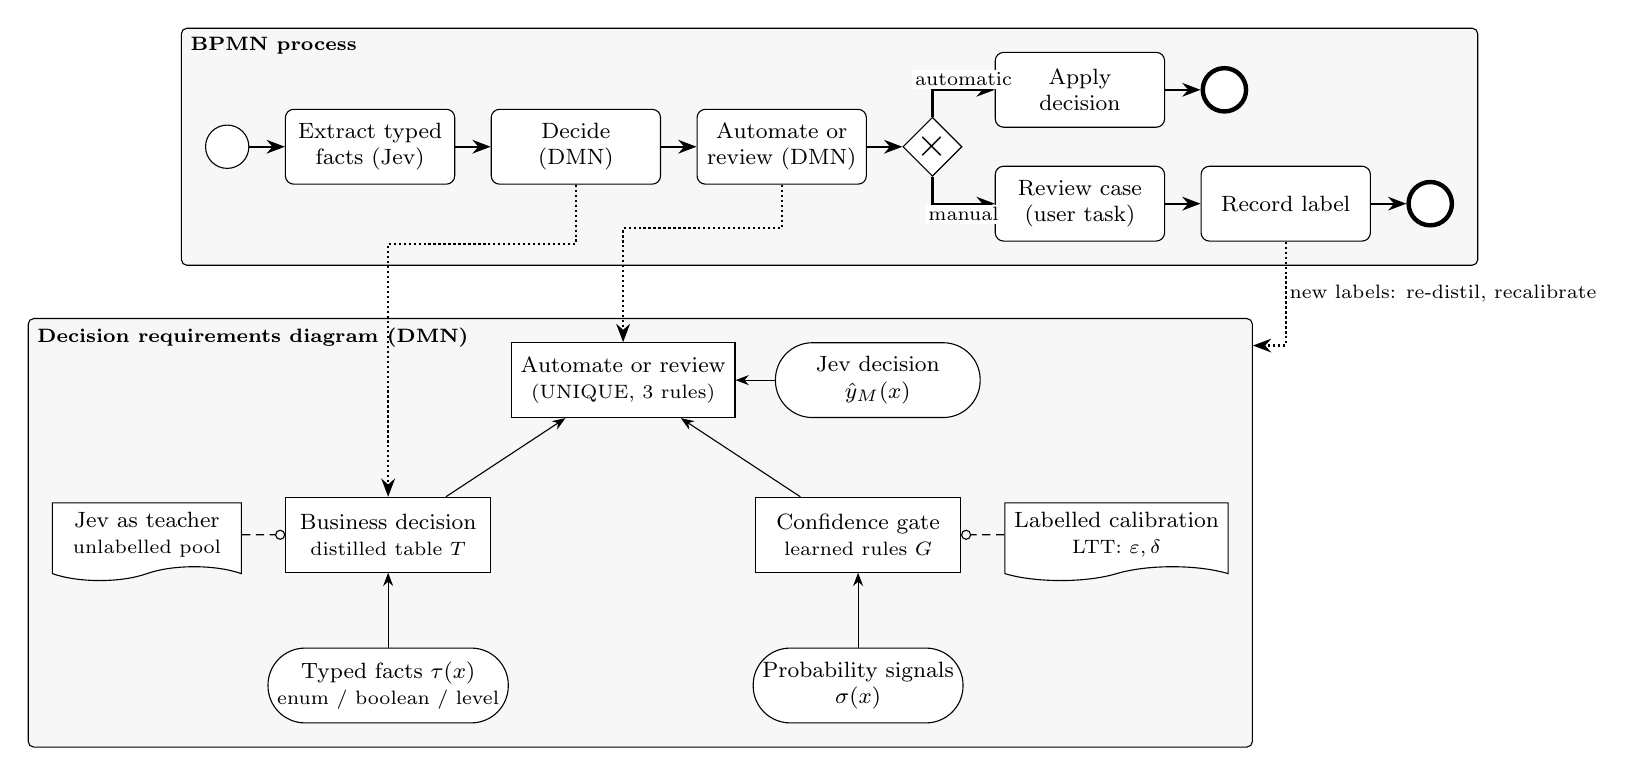
\begin{tikzpicture}[
    font=\footnotesize,
    >=Stealth,
    task/.style={draw, rounded corners=3pt, minimum width=2.15cm, minimum height=0.95cm, align=center, fill=white},
    event/.style={draw, circle, minimum size=0.55cm, fill=white},
    endevent/.style={draw, circle, line width=1.6pt, minimum size=0.55cm, fill=white},
    gateway/.style={draw, diamond, aspect=1, minimum size=0.75cm, inner sep=0pt, fill=white},
    decision/.style={draw, minimum width=2.6cm, minimum height=0.95cm, align=center, fill=white},
    input/.style={draw, rounded corners=0.47cm, minimum width=2.6cm, minimum height=0.95cm, align=center, fill=white},
    source/.style={draw, tape, tape bend top=none, minimum width=2.4cm, minimum height=0.95cm, align=center, fill=white},
    flow/.style={->, thick},
    req/.style={->, thin},
    auth/.style={-{Circle[open]}, densely dashed, thin},
    lbl/.style={font=\scriptsize, fill=white, inner sep=1pt},
  ]
  % ---------------- BPMN ----------------
  \node[event] (start) at (0,0) {};
  \node[task, right=0.45cm of start] (extract) {Extract typed\\facts (Jev)};
  \node[task, right=0.45cm of extract] (decide) {Decide\\(DMN)};
  \node[task, right=0.45cm of decide] (route) {Automate or\\review (DMN)};
  \node[gateway, right=0.45cm of route] (gw) {\Large$\times$};
  \node[task, above right=0.05cm and 0.6cm of gw] (apply) {Apply\\decision};
  \node[task, below right=0.05cm and 0.6cm of gw] (review) {Review case\\(user task)};
  \node[endevent, right=0.45cm of apply] (endA) {};
  \node[task, right=0.45cm of review] (record) {Record label};
  \node[endevent, right=0.45cm of record] (endB) {};
  \draw[flow] (start) -- (extract);
  \draw[flow] (extract) -- (decide);
  \draw[flow] (decide) -- (route);
  \draw[flow] (route) -- (gw);
  \draw[flow] (gw) |- node[lbl, pos=0.75, above] {automatic} (apply);
  \draw[flow] (gw) |- node[lbl, pos=0.75, below] {manual} (review);
  \draw[flow] (apply) -- (endA);
  \draw[flow] (review) -- (record);
  \draw[flow] (record) -- (endB);
  \begin{scope}[on background layer]
    \node[draw, fill=black!3, rounded corners=2pt, inner sep=0.3cm,
          fit=(start) (extract) (decide) (route) (gw) (apply) (review) (endA) (record) (endB),
          label={[anchor=north west, font=\scriptsize\bfseries]north west:BPMN process}] (bpmn) {};
  \end{scope}

  % ---------------- DRD ----------------
  \node[decision, below=2.0cm of decide, xshift=0.6cm] (outcome) {Automate or review\\{\scriptsize(UNIQUE, 3 rules)}};
  \node[decision, below left=1.0cm and 0.25cm of outcome] (business) {Business decision\\{\scriptsize distilled table $T$}};
  \node[decision, below right=1.0cm and 0.25cm of outcome] (gate) {Confidence gate\\{\scriptsize learned rules $G$}};
  \node[input, below=0.95cm of business] (facts) {Typed facts $\tau(x)$\\{\scriptsize enum / boolean / level}};
  \node[input, below=0.95cm of gate] (signals) {Probability signals\\$\sigma(x)$};
  \node[input, right=0.5cm of outcome] (holistic) {Jev decision\\$\hat y_{M}(x)$};
  \node[source, left=0.55cm of business] (teacher) {Jev as teacher\\{\scriptsize unlabelled pool}};
  \node[source, right=0.55cm of gate] (calib) {Labelled calibration\\{\scriptsize LTT: $\varepsilon,\delta$}};
  \draw[req] (facts) -- (business);
  \draw[req] (signals) -- (gate);
  \draw[req] (business) -- (outcome);
  \draw[req] (gate) -- (outcome);
  \draw[req] (holistic) -- (outcome);
  \draw[auth] (teacher) -- (business);
  \draw[auth] (calib) -- (gate);
  \begin{scope}[on background layer]
    \node[draw, fill=black!3, rounded corners=2pt, inner sep=0.3cm,
          fit=(outcome) (business) (gate) (facts) (signals) (holistic) (teacher) (calib),
          label={[anchor=north west, font=\scriptsize\bfseries]north west:Decision requirements diagram (DMN)}] (drd) {};
  \end{scope}
  \draw[->, densely dotted, thick] (decide.south) -- ++(0,-0.75) -| (business.north);
  \draw[->, densely dotted, thick] (route.south) -- ++(0,-0.55) -| (outcome.north);
  \draw[->, densely dotted, thick] (record.south) |- node[lbl, pos=0.25, right] {new labels: re-distil, recalibrate} ([yshift=-0.35cm]drd.north east);
\end{tikzpicture}
}
  \caption{Architecture. The BPMN process calls the System One model once per case and then evaluates a decision requirements diagram with three decisions. The business decision table is distilled from the model's own decisions (knowledge source on the left); the confidence gate is learned and thresholded on a labelled calibration set (knowledge source on the right). Cases decided by a reviewer produce labels for re-distillation and recalibration.}
  \label{fig:architecture}
\end{figure}

\begin{table}[pos=tbp]
  \centering
  \caption{Mapping of System One answer types to DMN. $p$ denotes the probability of the most likely answer; $n$ the number of options; $m^\star$ the most likely score level and $\bar d$ the mean absolute deviation of a uniform distribution over the levels.}
  \label{tab:types}
  \small
  \begin{tabular}{@{}llllp{4.3cm}@{}}
    \toprule
    Question & Model output & Typed value $\tau_j(x)$ & DMN type & Signals in $\sigma(x)$ \\
    \midrule
    Choice & distribution over $n\le 255$ options & most likely option & string, enumerated & $p$, confidence $\frac{p-1/n}{1-1/n}$, margin to 2nd \\
    Noul & probability of ``true'' & $p \ge 0.5$ & boolean & $p$, confidence $|2p-1|$ \\
    Score & distribution over $L\le 10$ levels & level $m^\star$ & number in $\{0,\dots,L-1\}$ & $p$, confidence $1-\frac{\sum_\ell \pi_\ell |\ell-m^\star|}{\bar d}$, margin \\
    \bottomrule
  \end{tabular}
\end{table}

Table~\ref{tab:types} gives the mapping from answers to DMN inputs. The typed value $\tau_j(x)$ is the most likely answer; together the typed values form the vector $\tau(x)\in D=D_1\times\dots\times D_m$. The signals $\sigma(x)$ summarise how certain each answer is; the confidence formulas are those of the vendor \citep{typesafe2026docs}. The model's holistic decision is $\hat y_M(x)=\arg\max_{c\in C}\pi_h(x)_c$ and the ground-truth decision, where available, is $y(x)$.

\subsection{Distilling the business decision table}\label{sec:distil}
The aim is a table $T: D\to C$ that reproduces $\hat y_M$ as closely as possible with as few rules as possible. Its \emph{fidelity} is $F(T)=\Pr[T(\tau(x))=\hat y_M(x)]$. Distillation needs no ground-truth labels: a pool $U$ of unlabelled cases is sent to $M$ once, and the pairs $(\tau(x),\hat y_M(x))$, $x\in U$, are the training data. Algorithm~\ref{alg:distil} summarises the procedure.

\begin{algorithm}[tbp]
  \caption{Distillation of a DMN decision table from a System One model.}
  \label{alg:distil}
  \small
  \KwIn{pool $U$; schema $(q_1,\dots,q_m,h)$; grids of depths and minimum leaf sizes; tolerance $t$}
  \KwOut{decision table $T$ with hit policy UNIQUE}
  Query $M$ once per $x\in U$; obtain $\tau(x)$ and $\hat y_M(x)$\;
  Encode $\tau(x)$: one-hot for choices, $0/1$ for nouls, integer level for scores\;
  Split $U$ into $U_{\mathrm{fit}}$ (80\%) and $U_{\mathrm{val}}$ (20\%)\;
  \ForEach{configuration $(d,\ell)$ in the grid}{
    Fit a CART tree of depth $\le d$ and leaf size $\ge \ell$ on $U_{\mathrm{fit}}$ with target $\hat y_M$\;
    $T_{d,\ell}\leftarrow$ \textsc{Merge}(\textsc{Paths}(tree)); record $|T_{d,\ell}|$ and fidelity on $U_{\mathrm{val}}$\;
  }
  Select the configuration with the fewest rules among those within $t$ of the best validation fidelity\;
  Refit it on $U$; \Return $T\leftarrow$ \textsc{Merge}(\textsc{Paths}(tree)) without unused inputs\;
\end{algorithm}

\paragraph{From paths to rules.} \textsc{Paths} turns each root-to-leaf path into one rule. Every split refers to an encoded column, which is mapped back to a condition on the original typed input: a split on the one-hot column for option $o$ of choice $q_j$ yields $\tau_j\in\{o\}$ or $\tau_j\in D_j\setminus\{o\}$; a split on a noul yields \feel{true} or \feel{false}; a split on a score yields a range of levels. Conditions on the same input are intersected along the path, so each rule assigns to every input a set $S_j\subseteq D_j$, written in FEEL as a list of values, a negated list (\feel{not("a","b")}), a range or \feel{-} when $S_j=D_j$. The rule's output is the majority class of its leaf; its support and purity are kept as rule annotations. Because the leaves of a tree partition the encoded space and every element of $D$ has exactly one encoding, the resulting rules partition $D$:

\begin{lemma}\label{lem:partition}
The rules produced by \textsc{Paths} are pairwise disjoint and cover $D$. Hence the table satisfies the UNIQUE hit policy and has no gaps on the whole input domain, not only on the observed cases.
\end{lemma}

The same translation applies to the gate, whose inputs are real-valued probabilities. A split $v\le\theta$ found on training values separates the largest value $a\le\theta$ from the smallest value $b>\theta$; any threshold $c\in[a,b)$ induces the same partition of the training data. We therefore write the shortest decimal in $[a,b)$, so that the table shows \feel{>= 0.88} rather than \feel{> 0.87645}, without changing any decision on the data the gate was fitted on.

\paragraph{Merging.} Two rules with the same output whose conditions coincide on all inputs but one, $j$, are replaced by a single rule with condition $S_j\cup S'_j$ (for real inputs only when the two intervals are adjacent, so that every cell remains one interval). As the two rules are disjoint boxes that differ in one dimension, their union is again a box and the table's semantics is unchanged; this is the merge step of \citet{calvanese2018}. We repeat merging to a fixpoint, grouping rules by their output and the conditions on all other inputs so that each pass is linear in the number of rules. Inputs that are \feel{-} in every rule are removed. For comparison we also report the size of an equivalent table with hit policy FIRST, in which the rules of the most frequent output are replaced by a final catch-all rule.

\paragraph{Model selection.} Fidelity usually grows with the number of rules while readability falls. Rather than fixing a size, we sweep tree depth and minimum leaf size and select the smallest table whose validation fidelity is within $t=1$ percentage point of the best; the full fidelity--complexity curve is reported.

\subsection{Verification}\label{sec:verify}
Lemma~\ref{lem:partition} holds by construction, but the exported artefact must also be checked. We verify each table in four ways. First, we compute all pairs of overlapping rules and the uncovered part of $D$ with box algebra: a rule is a box $\prod_j S_j$, two rules overlap if their conditions intersect on every input, and gaps are obtained by subtracting each rule from $D$, where the difference of two boxes is a union of at most $m$ disjoint boxes \citep{calvanese2018}. Second, the DRD is serialised to DMN~1.3 XML and validated against the OMG XML schema. Third, the XML is parsed back and its FEEL entries are evaluated by our own interpreter on every case; the outputs must equal those of the fitted tree. Fourth, an independent engine evaluates the same file: the DMN is parsed with \texttt{dmn-moddle} and its expressions and unary tests are evaluated with the FEEL interpreter \texttt{feelin} from the bpmn.io tool chain \citep{feelin}. Agreement of the four is required before a model is deployed.

\subsection{Risk-controlled confidence gate}\label{sec:gate}
Let $c(x)=\mathbb{1}[T(\tau(x))=y(x)]$ indicate that the table decides case $x$ correctly and $a(x)=\mathbb{1}[T(\tau(x))=\hat y_M(x)]$ that the table agrees with the model's holistic answer. A gate is a score $s(x)$ together with a threshold $\lambda$; a case is automated when $\tilde s(x)\ge\lambda$, where $\tilde s(x)=s(x)$ if $a(x)=1$ and $-\infty$ otherwise, so that disagreement always leads to review. The quantity a process owner cares about is the \emph{selective risk}
\begin{equation}
  R(\lambda)=\Pr\big[c(x)=0 \,\big|\, \tilde s(x)\ge\lambda\big],
\end{equation}
the error rate among automated cases, and the \emph{coverage} $\Pr[\tilde s(x)\ge\lambda]$, the share of cases automated. Given a tolerated error rate $\varepsilon$ and a failure probability $\delta$, we want the largest coverage such that $R(\lambda)\le\varepsilon$ holds with probability at least $1-\delta$.

\paragraph{Scores.} We compare two scores. The first is the model's own confidence in its holistic answer, $s(x)=\max_c\pi_h(x)_c$. The second is a \emph{learned gate}: a shallow classification tree (depth $\le 3$, at least 40 cases per leaf) fitted on the signals $\sigma(x)$ of the holistic question and of the facts used by $T$, with target $c(x)$; its score is the leaf estimate of $\Pr[c(x)=1]$. Because the tree is shallow, its leaves translate into a handful of readable DMN rules such as \feel{relief\_holistic\_\_conf >= 0.88}.

\paragraph{Threshold.} The labelled calibration set is split at random into halves $A$ and $B$. Half $A$ is used to fit the learned gate and to fix an ordered list of candidate thresholds $\lambda_1>\lambda_2>\dots>\lambda_K$ (Algorithm~\ref{alg:ltt}); half $B$ is used only for testing. For each candidate, let $n_k$ be the number of cases in $B$ with $\tilde s\ge\lambda_k$ and $e_k$ the number of errors among them. The null hypothesis $H_k: R(\lambda_k)>\varepsilon$ is tested with the exact binomial p-value $p_k=\Pr[\mathrm{Bin}(n_k,\varepsilon)\le e_k]$, and the hypotheses are tested in order until the first non-rejection.

\begin{algorithm}[tbp]
  \caption{Gate threshold by Learn-then-Test with fixed-sequence testing.}
  \label{alg:ltt}
  \small
  \KwIn{scores and correctness on halves $A$ and $B$; risk level $\varepsilon$; failure probability $\delta$; $K_{\max}$}
  \KwOut{threshold $\hat\lambda$ (accept $\tilde s\ge\hat\lambda$)}
  $n_{\min}\leftarrow\lceil \log\delta / \log(1-\varepsilon)\rceil$ \tcp*{fewest cases that can reject}
  On $A$: order distinct finite scores decreasingly; start at the first $\lambda$ for which a binomial test on $A$ rejects $H$ with at least $n_{\min}|A|/|B|$ accepted cases (else at the first with that many cases); keep $K_{\max}$ evenly spaced thresholds $\lambda_1>\dots>\lambda_K$\;
  $\hat\lambda\leftarrow+\infty$\;
  \For{$k=1,\dots,K$}{
    On $B$: $n_k\leftarrow|\{\tilde s\ge\lambda_k\}|$, $e_k\leftarrow$ errors among them, $p_k\leftarrow F_{\mathrm{Bin}(n_k,\varepsilon)}(e_k)$\;
    \lIf{$p_k>\delta$}{\textbf{break}}
    $\hat\lambda\leftarrow\lambda_k$\;
  }
  \Return $\hat\lambda$\;
\end{algorithm}

\begin{proposition}\label{prop:ltt}
Assume that the cases of half $B$ and future cases are independent and identically distributed and independent of half $A$ and of the pool used to build $T$. Then the threshold $\hat\lambda$ of Algorithm~\ref{alg:ltt} satisfies $\Pr\big[R(\hat\lambda)\le\varepsilon\big]\ge 1-\delta$.
\end{proposition}

\begin{proof}[Proof sketch]
Conditional on $A$ and the pool, the table, the score and the candidate list are fixed, so the hypotheses $H_1,\dots,H_K$ are fixed. Conditional on $n_k$, the cases of $B$ with $\tilde s\ge\lambda_k$ are an i.i.d.\ sample from the distribution of cases given $\tilde s\ge\lambda_k$, hence $e_k\sim\mathrm{Bin}(n_k,R(\lambda_k))$ and, under $H_k$, $\Pr[p_k\le u\mid n_k]\le u$ for all $u$; the p-value is therefore valid also unconditionally. Fixed-sequence testing rejects a true null only if the first true null in the sequence is rejected, which happens with probability at most $\delta$ whatever the dependence among the p-values; it thus controls the family-wise error rate at $\delta$ \citep{angelopoulos2025ltt}. If $R(\hat\lambda)>\varepsilon$, the true null $H_{\hat k}$ has been rejected, so $\Pr[R(\hat\lambda)>\varepsilon]\le\delta$.
\end{proof}

The guarantee does not require the model's probabilities to be calibrated; calibration only affects how many cases can be automated. Choosing the start of the sequence on $A$ matters in practice: fixed-sequence testing stops at the first non-rejection, and a sequence that starts at a threshold accepting only a few cases would stop immediately. When no candidate is rejected, $\hat\lambda=+\infty$ and every case is reviewed, which is the safe default.

\paragraph{Gate and outcome tables.} The learned gate is translated with \textsc{Paths}; each leaf outputs \feel{"auto"} if its score is at least $\hat\lambda$ and \feel{"review"} otherwise, and the rules are merged. The outcome decision is a three-rule UNIQUE table with inputs \emph{gate} and the FEEL expression \feel{business\_decision = holistic\_decision}; it returns \feel{"automatic"} only for (\feel{"auto"}, \feel{true}).

\subsection{Deployment and maintenance}
The DRD of Figure~\ref{fig:architecture} is deployed together with a BPMN process for Camunda~8: a service task calls the model and writes typed facts, signals and the holistic answer into process variables, two business rule tasks call the business and outcome decisions, and an exclusive gateway routes the case. Two knowledge sources document where the rules come from (the model version and the pool size) and how the gate was calibrated ($\varepsilon$, $\delta$, size of the calibration set). Because a model alias may move to a new version, the request pins a versioned model identifier and the response's model field is logged with every decision. Decisions made by reviewers become labels; they are used to monitor the selective risk in production and to recalibrate the gate or re-distil the table when the model, the case mix or the policy changes.

%% =======================================================================================
\section{Experimental design}\label{sec:design}

\subsection{Case and data}\label{sec:data}
We use the CFPB Consumer Complaint Database \citep{cfpb2026}, in which companies record how they closed each complaint; its narratives have been analysed, for example, with topic models to support complaint handling \citep{bastani2019}. The CFPB stopped publishing complaint narratives on 14~September~2026 \citep{cfpbnarratives2026}; we therefore take narratives from a public mirror of the database with complaints up to 2~January~2025 \citep{heineman2025} and join them by complaint identifier with the official bulk snapshot of 6~October~2026, which supplies the final company response. Only \res{data.labelchanged} of the joined complaints changed their response between the two snapshots, mostly from ``In progress'' to a final response. We keep complaints received between 1~April~2023 and 31~December~2024 with a narrative of at least 30 words, a closed response and a product in one of the ten product categories listed in Table~\ref{tab:tasks}, and drop exact duplicates of normalised narratives, which are common among templated letters and would otherwise leak between splits. This leaves \res{data.corpus} complaints.

\begin{table}[pos=tbp]
  \centering
  \caption{Decision tasks. Ground truth is derived from fields recorded by the CFPB; the model sees only the narrative.}
  \label{tab:tasks}
  \small
  \begin{tabular}{@{}p{2.3cm}p{5.6cm}p{6.3cm}@{}}
    \toprule
    Task & Cases and classes & Ground truth \\
    \midrule
    Monetary relief & \res{data.reliefn} random complaints about checking or savings accounts, credit and prepaid cards and money transfers; classes \feel{relief}, \feel{no\_relief} (\res{data.reliefpos} relief) & company response ``Closed with monetary relief'' versus ``Closed with explanation'' or ``Closed with non-monetary relief'' \\
    \addlinespace
    Routing & \res{data.routingn} complaints, \num{1250} per queue; eight queues: credit reporting, debt collection, deposits, cards, payments, mortgage, consumer loans, fraud & product group selected by the consumer; complaints whose issue or sub-issue denotes fraud, identity theft or unauthorised activity go to the fraud queue (14 issue/sub-issue pairs, listed in the repository) \\
    \bottomrule
  \end{tabular}
\end{table}

From this corpus we draw two samples with a fixed seed (Table~\ref{tab:tasks}). The relief task is a real business decision taken by the company after handling the complaint; among the \res{data.banking} banking complaints of the corpus, \res{data.bankingrelief} were resolved with monetary relief. The routing task uses the consumer's own classification as a proxy for the correct handling queue, simulating an intake channel such as e-mail or a call centre where no category is selected; the fraud queue makes the routing depend on more than the product. The union of both samples has \res{data.sample} complaints with a median length of \res{data.wordsmedian} words (interquartile range \res{data.wordsiqr}); \res{data.truncated} narratives longer than 1{,}500 words are truncated. Each task is split, stratified by its ground truth, into a pool (60\%), a calibration set (20\%) and a test set (20\%): \res{data.reliefpool}/\res{data.reliefcalibration}/\res{data.relieftest} cases for relief and \res{data.routingpool}/\res{data.routingcalibration}/\res{data.routingtest} for routing. Ground truth of the pool is never used by the distilled table.

\subsection{Question schema}\label{sec:schema}
All questions of both tasks are asked in a single request per complaint, with the narrative as the state. The schema (Table~\ref{tab:schema}) has fourteen fact questions and two holistic questions. The facts describe the complaint, not the decision: what product it concerns, whether the consumer reports unauthorised activity, a loss of money, a refund request or a denied claim, and how much financial harm is described. Following the vendor's guidance \citep{typesafe2026jagged}, every question states one literal condition, avoids arithmetic and dates and adds an explicit ``other'' option where the answer may not exist. Neither holistic question mentions the facts, so that the distilled table has to discover how the model's holistic judgement relates to them.

\begin{table}[pos=tbp]
  \centering
  \caption{Question schema (abridged wording; full text in the repository). C = choice, N = noul, S = score.}
  \label{tab:schema}
  \footnotesize
  \begin{tabular}{@{}llp{11.6cm}@{}}
    \toprule
    Id & Type & Question \\
    \midrule
    \feel{product} & C (11) & Which financial product or service is the complaint mainly about? (ten products, ``other'') \\
    \feel{unauthorized} & N & A transaction, charge, withdrawal or account was made without the consumer's permission. \\
    \feel{identity\_theft} & N & The consumer is a victim of identity theft. \\
    \feel{scam} & N & A scammer tricked the consumer into sending money or giving account access. \\
    \feel{report\_dispute} & N & The consumer disputes information on their credit report. \\
    \feel{collector\_contact} & N & The consumer complains about contact from a debt collector. \\
    \feel{money\_lost} & N & The consumer lost money or was charged money they believe they should not have paid. \\
    \feel{fee\_or\_interest} & N & The complaint is about a fee, a penalty or an interest charge. \\
    \feel{refund\_requested} & N & The consumer asks for a refund, reimbursement, credit or return of money. \\
    \feel{prior\_contact} & N & The consumer contacted the company about the problem before complaining. \\
    \feel{company\_admitted} & N & The company admitted a mistake or promised to fix the problem. \\
    \feel{claim\_denied} & N & The company denied or rejected the consumer's dispute, claim or request. \\
    \feel{funds\_blocked} & N & The consumer cannot use their account or money because the company froze, held, restricted or closed it. \\
    \feel{harm} & S (4) & How much financial harm is described? (none; small; significant or ongoing; severe) \\
    \midrule
    \feel{relief\_holistic} & N & Based on the complaint, the company should refund or reimburse money to the consumer. \\
    \feel{queue\_holistic} & C (8) & Which team should handle this complaint? (eight queues with one-line descriptions) \\
    \bottomrule
  \end{tabular}
\end{table}

\subsection{Model and protocol}
We call \jev{} through the System One API with the pinned model \texttt{jev-1.13.0} (reported model: \res{relief.models}). Each complaint is sent once; the request, the raw response, the latency and the time stamp are stored, and all analyses read from this record. Decision trees use scikit-learn \citep{pedregosa2011} with depths $\{1,\dots,6,8,10,12,\text{unbounded}\}$ and minimum leaf sizes $\{5,20,50,100\}$. The gate is calibrated for $\varepsilon\in\{0.01,0.02,0.05,0.10\}$ with $\delta=0.05$; the gate exported to DMN uses $\varepsilon=0.05$.

\subsection{Baselines}
We compare the distilled table (\emph{Jev+DMN, distilled}; no ground-truth labels) with: the majority class; \jev{}'s holistic answer (\emph{Jev holistic}; no labels); a decision table learned with the same procedure on \jev{}'s typed facts but with ground-truth labels as target (\emph{Jev+DMN, supervised}); and a TF-IDF representation of the narrative (word uni- and bigrams) with logistic regression (\emph{TF-IDF+LR}), a strong supervised text classifier without auditable logic. The supervised baselines are trained on labelled subsets of the pool of $\{100, 250, 500, 1000, 2000\}$ cases (five random repetitions) and on the whole pool, which shows how many labels they need to match the label-free approach. For the gate we compare no gate, the agreement filter alone, \jev{}'s confidence and the learned gate, each with and without the agreement filter.

\subsection{Metrics and statistical analysis}
Fidelity is the agreement between the table and \jev{}'s holistic answer on the test set, with Cohen's $\kappa$ \citep{cohen1960} and a 95\% percentile-bootstrap interval (2{,}000 resamples). Accuracy and macro-averaged F1 are computed against the ground truth. Calibration is measured by the top-label ECE with 15 equal-width bins (and equal-mass bins), the maximum calibration error, the multi-class Brier score \citep{brier1950} and reliability diagrams; isotonic recalibration is fitted on the calibration set and evaluated on the test set. For the gate we report coverage and selective risk on the test set, the area under the risk--coverage curve (AURC), and an empirical check of Proposition~\ref{prop:ltt}: the calibration and test cases are pooled and repeatedly split at random into $A$, $B$ and an evaluation part (200 repetitions), and we count how often the selective risk on the evaluation part exceeds $\varepsilon$. Paired accuracy differences are tested with the exact McNemar test \citep{mcnemar1947}. Table complexity is the number of rules, the number of inputs and the mean number of non-trivial conditions per rule. Operational metrics are the model latency per case (median and 95th percentile), the time to evaluate the table, the cost per 1{,}000 cases at the published price of \$0.042 per million input tokens, and the number of cases per 1{,}000 sent to review.

\subsection{Implementation}
The method is implemented in Python. The DMN writer produces DMN~1.3 XML with diagram interchange information, so the models open in DMN modelling tools; the BPMN model uses Camunda~8 extensions. The code, the question schema, the identifiers of all sampled complaints with their splits, the generated DMN and BPMN models and the scripts that produce every number and figure of this paper are available in the repository (Section~\ref{sec:data-availability}).

%% =======================================================================================
\section{Results}\label{sec:results}
%% NOTE: every number below is generated from results/jev by scripts/make_paper_assets.py.
%% Interpretive sentences marked TODO are to be written once the Jev run is complete.

\subsection{RQ1: Fidelity and complexity of distilled tables}\label{sec:res-rq1}
Table~\ref{tab:distillation} summarises the distilled tables. For the relief decision the selected table has \res{relief.rules} rules over \res{relief.inputs} inputs and reproduces \jev{}'s holistic decision on \res{relief.fidelity} of the test cases (95\% CI \res{relief.fidelityci}; $\kappa=\res{relief.kappa}$). For routing it has \res{routing.rules} rules over \res{routing.inputs} inputs with a fidelity of \res{routing.fidelity} (95\% CI \res{routing.fidelityci}; $\kappa=\res{routing.kappa}$). Merging reduced the tables from \res{relief.rulesraw} and \res{routing.rulesraw} tree leaves; with a FIRST hit policy and a default rule they need \res{relief.rulesfirst} and \res{routing.rulesfirst} rules. All tables passed every verification step: no conflicting overlaps and no gaps (as Lemma~\ref{lem:partition} predicts), XSD-valid XML, and identical outputs of the tree, our FEEL interpreter and the independent engine on all cases (round-trip agreement \res{relief.roundtrip} and \res{routing.roundtrip}). Figure~\ref{fig:complexity} shows the fidelity--complexity trade-off over all configurations. Table~\ref{tab:rules} shows the relief table as it appears in the DMN model.
% TODO(after Jev run): interpret which facts the tables use and where fidelity saturates.

\begin{table}[pos=tbp]
  \centering
  \caption{Distilled business decision tables (test set). Fidelity is agreement with \jev{}'s holistic decision; overlaps/gaps after merging.}
  \label{tab:distillation}
  \small
  \gentable{tab_distillation}
\end{table}

\begin{figure}[pos=tbp]
  \centering
  \genfigure{fig_complexity}
  \caption{Fidelity to \jev{} against the number of rules for all configurations of the sweep, refitted on the pool and evaluated on the test set. The step line is the Pareto front; the diamond marks the selected table.}
  \label{fig:complexity}
\end{figure}

\begin{table}[pos=tbp]
  \centering
  \caption{Distilled decision table for monetary relief (inputs that are ``\feel{-}'' in every rule omitted; support = pool cases per rule).}
  \label{tab:rules}
  \footnotesize
  \gentable{tab_rules_relief}
\end{table}

\subsection{RQ2: Calibration}\label{sec:res-rq2}
Table~\ref{tab:calibration} and Figure~\ref{fig:reliability} report how well \jev{}'s holistic probabilities match the true outcomes. On the test set, \jev{}'s holistic answer is correct for \res{relief.accholistic} of relief cases at a mean confidence of \res{relief.meanconf} (ECE \res{relief.ece}, Brier \res{relief.brier}) and for \res{routing.accholistic} of routing cases at a mean confidence of \res{routing.meanconf} (ECE \res{routing.ece}, Brier \res{routing.brier}). Isotonic recalibration on the calibration set changes the ECE to \res{relief.eceiso} and \res{routing.eceiso}, respectively.
% TODO(after Jev run): over- or under-confidence; does the vendor's calibration claim transfer to these tasks?

\begin{table}[pos=tbp]
  \centering
  \caption{Calibration of \jev{}'s holistic answer against the ground truth (test set).}
  \label{tab:calibration}
  \small
  \gentable{tab_calibration}
\end{table}

\begin{figure}[pos=tbp]
  \centering
  \genfigure{fig_reliability}
  \caption{Reliability diagrams of \jev{}'s top-label confidence on the test set, raw and after isotonic recalibration (bins with at least 10 cases).}
  \label{fig:reliability}
\end{figure}

\subsection{RQ3: Automation under a risk constraint}\label{sec:res-rq3}
Table~\ref{tab:gate} reports, for each gate and risk level, the share of test cases decided automatically and the error rate among them; Figure~\ref{fig:riskcov} shows the full risk--coverage curves. The table agrees with \jev{}'s holistic answer on \res{relief.agreerate} of relief and \res{routing.agreerate} of routing test cases; when it agrees, it is correct on \res{relief.accagree} and \res{routing.accagree} of the cases, and when it disagrees on \res{relief.accdisagree} and \res{routing.accdisagree}. At $\varepsilon=0.05$, the learned gate with the agreement filter automates \res{relief.learnedA.5.cov} of relief cases with an error rate of \res{relief.learnedA.5.risk}, and \res{routing.learnedA.5.cov} of routing cases with an error rate of \res{routing.learnedA.5.risk}. The AURC of the learned gate is \res{relief.aurclearned} (relief) and \res{routing.aurclearned} (routing), against \res{relief.aurcconf} and \res{routing.aurcconf} for \jev{}'s confidence. In the repeated-splitting check, the selective risk exceeded $\varepsilon=0.05$ in \res{relief.violation5} (relief) and \res{routing.violation5} (routing) of the 200 repetitions, against the nominal $\delta=5\%$.
% TODO(after Jev run): interpret contrast between tasks; which signals does the learned gate use?

\begin{table}[pos=tbp]
  \centering
  \caption{Coverage (Cov., \% of test cases automated) and selective risk (Risk, \% errors among automated cases) of the confidence gates, $\delta=0.05$. ``--'' marks levels at which no threshold was certified and all cases go to review.}
  \label{tab:gate}
  \footnotesize
  \gentable{tab_gate}
\end{table}

\begin{figure}[pos=tbp]
  \centering
  \genfigure{fig_risk_coverage}
  \caption{Risk--coverage curves on the test set (agreement filter not applied), with the risk levels $\varepsilon$ used for calibration.}
  \label{fig:riskcov}
\end{figure}

\subsection{RQ4: Comparison with baselines and operational cost}\label{sec:res-rq4}
Table~\ref{tab:baselines} compares the approaches. Without any labels, the distilled table reaches an accuracy of \res{relief.accdmn} on relief and \res{routing.accdmn} on routing, against \res{relief.accjev} and \res{routing.accjev} for \jev{}'s holistic answer (exact McNemar test: $p=\res{relief.mcnemarp}$ and $p=\res{routing.mcnemarp}$). With all \res{relief.labelsfull} (relief) and \res{routing.labelsfull} (routing) pool labels, the supervised table reaches \res{relief.accsupfull} and \res{routing.accsupfull}, and TF-IDF+LR \res{relief.acctfidffull} and \res{routing.acctfidffull}. Figure~\ref{fig:learning} shows how the supervised baselines depend on the number of labels.

The model answered a request with all sixteen questions in a median of \res{relief.latmed}~ms (95th percentile \res{relief.latp95}~ms) at a mean of \res{relief.tokens} input tokens, which corresponds to \$\res{relief.cost} per 1{,}000 cases. Evaluating the distilled table took \res{relief.dmnus}~$\mu$s per case in our Python implementation. At $\varepsilon=0.05$ the relief process sends \res{relief.review} and the routing process \res{routing.review} of every 1{,}000 cases to review.
% TODO(after Jev run): option-order robustness (reversed choice options on a random subset of test cases).
% TODO(after LLM key): LLM baseline with structured output via system-one-adapter (same questions).

\begin{table}[pos=tbp]
  \centering
  \caption{Accuracy against ground truth on the test set. Labels = ground-truth labels used for training; supervised results with all pool labels.}
  \label{tab:baselines}
  \small
  \gentable{tab_baselines}
\end{table}

\begin{figure}[pos=tbp]
  \centering
  \genfigure{fig_learning}
  \caption{Test accuracy of supervised baselines against the number of training labels (mean $\pm$ standard deviation over five draws), compared with the two label-free approaches.}
  \label{fig:learning}
\end{figure}

%% =======================================================================================
\section{Discussion}\label{sec:discussion}

\subsection{Implications for research}
The method separates three concerns that black-box automation entangles: reading the case, deciding, and deciding whether to decide. Reading is delegated to a model with typed output; deciding is done by a table that a person can read and that an engine executes; whether to decide is governed by a second table whose threshold carries a statistical guarantee. Each part can be inspected and replaced independently. This extends decision discovery \citep{bazhenova2016,desmedt2019,etinger2019} from structured logs to unstructured input, and it turns the abstract idea of a concept bottleneck \citep{koh2020} into an artefact of an industry standard.

Distillation from a model with typed output avoids two problems of distilling from free-text LLM output. There is nothing to parse: every answer is a value of a declared type, so the student's inputs are well defined. And the teacher's labels come with probabilities, which a text-generating model provides only through token likelihoods or verbalised confidence \citep{kadavath2022,xiong2024}. Fidelity measures how much of the model's holistic judgement can be expressed through the chosen facts; low fidelity is itself informative, because it signals that the schema misses a factor the model uses.
% TODO(after Jev run): relate fidelity and accuracy findings to this argument.

The confidence gate uses calibration data only where it is needed. Proposition~\ref{prop:ltt} holds whether or not the model is calibrated, so a process owner can rely on the stated error bound even for a model whose calibration on the task is unknown. Calibration, which RQ2 measures, determines how many cases the bound allows to be automated.

\subsection{Implications for practice}
For organisations, the approach provides a path to automating decisions on unstructured input that fits existing governance. The decision logic lives in a DMN table that business analysts can review and change through the usual change process; the knowledge sources in the DRD document which model version and which calibration data the rules come from. A risk owner sets $\varepsilon$ per decision, as with the different thresholds for low- and high-stakes actions in the vendor's guidance \citep{typesafe2026docs}, and the gate shows the price of that choice in reviewer workload. Every automated decision can be explained by the rule that fired and the facts that matched, which supports the transparency and human-oversight obligations of the AI Act \citep{euaiact2024}. Because the model is called once per case and the table evaluation is negligible, the latency and the cost per case are those of a single model request.

\subsection{Limitations and threats to validity}
\emph{Construct validity.} The ground truth of the relief task is what companies did, not what they should have done; relief also depends on company policies and on facts not in the narrative. The routing ground truth is the consumer's own choice of product and issue, which is a proxy for the correct queue. Both are noisy and bound the achievable accuracy of every method.

\emph{Internal validity.} Splits are stratified and fixed by a seed, the pool's labels are never used by the distilled table, calibration and test sets are disjoint, and exact duplicate narratives are removed. Near-duplicates may remain. The schema was designed before the experiments and was not tuned on the test set; a different schema would lead to different tables, and schema design is part of the method rather than a free parameter.

\emph{External validity.} We study one domain, one language and one model. \jev{} is a commercial model in early access whose weights are not available, so its results cannot be reproduced bit for bit; we mitigate this by pinning the model version, storing every request and response, and releasing the complaint identifiers. The method only assumes typed questions with probability distributions over answers, so it applies to other models of the class. An open adapter that emulates the System One interface with LLMs \citep{systemoneadapter} makes a reproduction with open models possible, at different latency and cost. The narratives come from a public mirror because the CFPB withdrew them from its database; the identifiers and the mirror's checksums are released so that the sample can be reconstructed.

\emph{Statistical validity.} Proposition~\ref{prop:ltt} assumes that future cases are exchangeable with the calibration cases. Changes in the case mix, the company policy or the model version break this assumption and require recalibration, for which the process supplies the labels.

%% =======================================================================================
\section{Conclusion}\label{sec:conclusion}
We showed how a System One model, which answers typed questions with probability distributions, can be turned into an auditable decision service in DMN. The model teaches a decision table over its own typed answers, which is verified and executed by a standard engine, and its probabilities drive a confidence gate whose threshold bounds the error rate of automated cases with a chosen probability. On \res{data.sample} complaints from the CFPB and two complaint-handling decisions we measured the fidelity and size of the distilled tables, the calibration of the model, the share of cases that can be automated at a given risk, and the trade-offs against the model alone and against supervised alternatives.
% TODO(after Jev run): one-sentence summary of the main quantitative findings.
Future work will apply the method to processes with richer state, combine distillation with the labels that reviewers produce, and study how tables and gates should be maintained when the underlying model is updated.

%% =======================================================================================
\section*{CRediT authorship contribution statement}
\printcredits

\section*{Declaration of competing interest}
%% TODO(authors): confirm. Mention any relationship with TypeSafe AI (e.g., early-access credits).
The authors declare that they have no known competing financial interests or personal relationships that could have appeared to influence the work reported in this paper.

\section*{Declaration of generative AI and AI-assisted technologies in the manuscript preparation process}
During the preparation of this work the author(s) used Claude (Anthropic) to assist with software development and with drafting and editing the manuscript. After using this tool, the author(s) reviewed and edited the content as needed and take(s) full responsibility for the content of the published article.

\section*{Data availability}\label{sec:data-availability}
%% TODO(authors): insert repository URL and archive DOI (e.g., Zenodo) before submission.
Code, question schema, complaint identifiers with splits, generated DMN and BPMN models, raw model responses and analysis scripts will be made available at [repository URL]. The complaint data are public \citep{cfpb2026,heineman2025}.

\section*{Funding}
%% TODO(authors): funding statement.
This research did not receive any specific grant from funding agencies in the public, commercial, or not-for-profit sectors.

\bibliographystyle{cas-model2-names}
\bibliography{refs}

\end{document}
